% This is the Oregon State University LaTeX template. To the best of my
% knowledge, most of the work was done by those acknowledged in beavtex.cls.

%%
%% Preamble
%%
% \documentclass{<something>} must begin each LaTeX document
\documentclass[double,11pt]{beavtex}
% Added by ZNK -- indent first paragraph after section.
\usepackage{indentfirst}
% Added by CII
\usepackage{graphicx,latexsym}
\usepackage{amsmath}
\usepackage{amssymb,amsthm}
\usepackage{longtable,booktabs,setspace}
\usepackage[hyphens]{url}
\usepackage[colorlinks = true,
			urlcolor = blue,
			linkcolor = black,
			citecolor = black,
			anchorcolor = black]{hyperref}
\usepackage{lmodern}
\usepackage{float}
\floatplacement{figure}{H}
% End of CII addition
\usepackage{rotating} % Package added to allow the rotation of figures and chart
                      % on a page, {sidewaysfigure} command
\usepackage{tablefootnote} % Packaged added to allow footnotes in the tabular
                           % environment, use \tablefootnote command

% This has to do with a default pandoc thing
% http://tex.stackexchange.com/a/258486/77699
\providecommand{\tightlist}{%
  \setlength{\itemsep}{0pt}\setlength{\parskip}{0pt}}

% Added by CII (Thanks, Hadley!)
% Use ref for internal links
\renewcommand{\hyperref}[2][???]{\autoref{#1}}
\def\chapterautorefname{Chapter}
\def\sectionautorefname{Section}
\def\subsectionautorefname{Subsection}
% End of CII addition

% Added by CII
\usepackage{caption}
\captionsetup{width=5in}
% End of CII addition

\title{Development and Application of Tools for Genetic Analysis of Clonal
Populations} % {An Analysis of Something}
\author{Zhian N. Kamvar} % {Joseph A. Student}
\degree{Doctor of Philosophy} % {Master of Science}
\doctype{Dissertation}
\submitdate{December 6, 2016} % {January 1, 2013}
\commencementyear{2017} % {2013}

\department{Botany and Plant Pathology} % {Nuclear Engineering and Radiation Health Physics}

\depttype{Department} % {School}

\depthead{Head} % {Director}

\major{Botany and Plant Pathology} % {Radiation Health Physics}

\advisor{Niklaus J. Grünwald} % {Jane R. Professor}

\abstract{Research on the population genetics of microbial organisms requires the
use of specialized analyses designed for clonal organisms to avoid
violating the assumptions of traditional population genetic models. The
tools necessary for performing these analyses existed as a set of
unrelated software with non-overlapping capabilities and did not cover
all aspects of analysis. This meant that researchers not only had to
reshape their data into different formats for each analysis, but they
also had to switch computing platforms, thus creating a drain in time,
and increasing the risk of propagating human error into the analysis. To
address this problem, we created the software package \emph{poppr},
written in the R statistical language, available on all computing
platforms. This package is designed for analysis of clonal, partially
clonal, and sexual populations, empowering researchers to perform their
work in a reproducible manner. We additionally demonstrate the utility
of \emph{poppr} for both plant pathological and theoretical questions by
using real-world and simulated data. In chapter 4, we apply these new
tools to demonstrate evidence for at least two origins for the outbreak
of the Sudden Oak Death pathogen, \emph{Phytophthora ramorum} in Curry
County, Oregon. In chapter 5, we use \emph{poppr} to assess the power of
the index of association with clone-correction, showing that
clone-correction has the potential to reduce the power of detecting
clonal reproduction. All of the software and analyses in this work were
performed in an open and reproducible framework, serving as an example
of the power of reproducible research in plant pathology.}
\acknowledgements{A Ph. D. student is nothing without the support of her/his community.
For this support, I am ever grateful for the Department of Botany and
Plant Pathology and the USDA ARS Horticultural Crops Research Laboratory
for providing me with a home for the past 5 years. I must thank my
advisor, Niklaus J. Grünwald for providing me with the tools and
challenges necessary for me to succeed. I thank my committee members,
Gail Langellotto, Chris Mundt, Michael Blouin, and Joey Spatafora for
their immense patience and understanding whenever I came to them stuck
in a well of my own thoughts. I am ever grateful to Joyce Loper, Brenda
Shaffer, Jeff Chang, Jerry Weiland, and Walt Mahaffee for long and
winding conversations on the nature of graduate school and science. The
Hansen lab graciously hosted me and my \emph{Phytophthora} samples
during the October 2013 government shutdown. Paul Reeser, Wendy Sutton,
Sarah Navarro, Laura Sims, and Everett Hansen taught me a lot about the
biology of \emph{Phytophthora}. I also would like to thank Val Fieland,
Meg Larsen, Caroline Press, and Karan Fairchild for teaching me to
culture \emph{Phytophthora}, and keeping the Grünwald lab running
smoothly despite my best efforts to introduce chaos. I also wish to
thank Dianne Simpson, Carleen Nutt, and Blaine Baker for providing a
sanctuary of sarcastic jokes and for keeping BPP together. I also want
to thank my wonderful undergraduate mentees, Ciera Gray and Jonah
Brooks. It was a fantastic opportunity to get to see both of you grow
and apply your skills.

I could not have made it through graduate school without the patience
and support of Sydney E. Everhart and Brian J. Knaus, who were always
willing to sit down and talk about everything from population genetic
theory, writing style, to life in general. These two were responsible
for guiding me through much of the research and writing before it ever
went to my advisor. Most importantly, Sydney and Brian gave me
encouragement even if I was being down on myself.

If it weren't for the guidance and mentoring of my undergraduate
research advisors, Drs. Brent Buckner and Dianne Janick-Buckner, I might
never have pursued graduate education. They recognized that grades did
not always reflect the intelligence or potential of a student. They
brought me into their research team, and I can't possibly thank them
enough for that.

My work absolutely could not have been done without the support of the
wider R and open source community. Without open codebases, \emph{poppr}
would have broken a long time ago. I wish to thank Thibaut Jombart for
always being open and accepting of my suggestions for improvements to
\emph{adegenet}, which in turn, improved \emph{poppr}. Thanks also goes
to C. Titus Brown for helping me with questions I had about the nature
of open science and reproducible research.

I also thank all the graduate students for being such a strong community
for all of us to debate, celebrate, and commiserate. I especially need
to thank (in no particular order) M. Quamar Salih, J. Caity Smyth, Hank
Raizen, Sarah Navarro, Joey Hulbert, Top Jimmy Klick, Lorena Rangel,
Rachel Bomberger, Lindsey Thiessen, Javier F. Tabima R., Alija Bajro
Mujic (word), Christina Hagerty, Hannah Rivedal, Kat Sweeny, Kevin
Weitemier, Trang Dang, Danielle Tom, Shankar ``Shanks'' Shakya, Zach
S.L. Foster, Alisha Owensby Quandt, Chris Hedstrom, Dani Lightle, Derek
Johnson, Thomas Stokely, Tyler Schappe (for endless Simpsons quotes),
Kristen Finch, Brian Atkinson, Phil Schapker, Mara Friddle, Jeremy
Hoffman, Braden Elliot, Biz Stamm, Chris Benemann, Daniel Henry Farber,
John Yeo, Alfredo Diaz, Pat DiBello, Megan O'Malley, Gray Rozabach, Nash
Irongay, Sam Colby, Lea Condon, Dabao Lu, and Pat Bennett. All of these
people and more have contributed to my well being in one way or another
and I can't possibly thank them enough for it. I also need to thank
everyone at the Coalition of Graduate Employees who taught me the
strength of community, especially, but not limited to, Ashley Bromley,
(K)Sean McGregor, Béatrice Moissinac, Kris Osterloh, Chris Mihiar,
Stephanie Parreira, Thomas Morrill, Vance Almquist, Clint Mattox, and
Dixie Daniels.

Special thanks goes to Joseph Michael Hulbert. Together with his drive
and ambition, we created the radio show Inspiration Dissemination which
has to date interviewed over 150 graduate students from Oregon State
University. This show has provided a valuable outlet for me and it would
not be possible without the undying dedication from Joey. In turn, I
would like to thank Matthew Spence McConnell for not only picking up the
torch from Joey, but also for continuing to improve the show and attract
a wider range of graduate students to be featured. I am additionally
thankful for the hosts who will take the show to a glorious future,
Kristen Finch, Adrian Gallo, Steve Friedman, Mackenzie Smith, and Lillie
Padgitt-Cobb. I want to thank all of the guests who have come on the
show and told your stories. Lastly, I need to thank all of the people at
KBVR who have supported the show throughout the years, especially: Kurt
Hagan, Jodie Davaz, Matt Walton, Rose Kearsey, Anthony Heatherly, and
Jack Kemp. Radio has always been an escape for me and I'm thankful for
the people who helped me be a part of it.

For many, the writing of the introduction and conclusion to a
dissertation is one of the most difficult tasks. I want to thank Robin
Choudhury, Brian Knaus, Danielle Tom, and Nik Grünwald for taking time
to be sounding boards for the structure of the introduction and
conclusion of this dissertation.

Finally, I need to thank my family for their enduring patience; my
mother, Jane H. Kamvar, my sister Margo Cartwright, and my brother
Rostam Kamvar. The most thanks must of course go to my wonderful spouse,
Jimin Im Kamvar. Without her, my life would have no color or balance.
She was the only one who could keep me going when all seemed hopeless.

I must additionally acknowledge my funding for my Ph. D.: US Department
of Agriculture (USDA) Agricultural Research Service Grant
5358-22000-039-00D, USDA APHIS, the USDA-ARS Floriculture Nursery
Initiative, the Oregon Department of Agriculture/Oregon Association of
Nurseries (ODA-OAN), the USDA-Forest Service Forest Health Monitoring
Program, the Department of Botany and Plant Pathology for providing me
with two terms of valuable teaching experience, as well as a generous
travel grant from the Anita Summers foundataion. The Oregon State
University Graduate School provided me with a \$500 travel grant and
NESCent provided me with airfare to attend the Population Genetics in R
Hackathon in Charlotte, NC. This helped me get in contact with Thibaut
Jombart, the maintainer of \emph{adegenet}, allowing me to contribute
significant improvements, which helped immeasurably to the improvement
of \emph{poppr} and Chapter 3. Finally, I must acknowledge the Botany
and Plant Pathology Graduate Student Association and the American
Phytopathological Society Foundation for providing me with funding to
attend the 2016 APS Annual Meeting in Tampa, FL.}


	\contributors{The following people contributed to this dissertation:

\subsubsection*{Chapter 2}\label{chapter-2}
\addcontentsline{toc}{subsubsection}{Chapter 2}

Zhian N. Kamvar conceived and designed the experiments, performed the
experiments, analyzed the data, contributed reagents/materials/analysis
tools, wrote the paper, prepared figures and tables, reviewed drafts of
the paper.

Javier F. Tabima conceived and designed the experiments, performed the
experiments, analyzed the data, contributed reagents/materials/analysis
tools, prepared figures and tables, reviewed drafts of the paper.

Niklaus J. Grünwald conceived and designed the experiments, analyzed the
data, contributed reagents/materials/analysis tools, wrote the paper,
reviewed drafts of the paper.

\subsubsection*{Chapter 3}\label{chapter-3}
\addcontentsline{toc}{subsubsection}{Chapter 3}

Zhian N. Kamvar and Jonah C. Brooks wrote and tested the code. Zhian N.
Kamvar and Niklaus J. Grünwald conceived, discussed implications, and
wrote the manuscript. Niklaus J. Grünwald coördinated the collaborative
effort.

\subsubsection*{Chapter 4}\label{chapter-4}
\addcontentsline{toc}{subsubsection}{Chapter 4}

Zhian N. Kamvar designed and ran the computational analyses, interpreted
the results, and wrote the manuscript Meredeth M. Larsen extracted DNA
and genotyped isolates of \emph{P. ramorum} from 2013 and 2014 at 14
microsatellite loci, harmonized the data between labs and wrote the
genotyping methods for the manuscript. Alan M. Kanaskie collected
\emph{P. ramorum} isolates from infected plant material, performed field
surveys, GIS work, and geotagging with the Brooking SOD ground crew and
assisted with writing of the manuscript, Everett M. Hansen provided
data, strains were isolated by Paul Reeser and Wendy Sutton, and
genotyped by Jen Britt. Everett M. Hansen assisted with writing the
manuscript, and Niklaus J. Grünwald conceived the study, analyzed the
data, contributed reagents/materials/analysis tools, and wrote the
paper.

\subsubsection*{Chapter 5}\label{chapter-5}
\addcontentsline{toc}{subsubsection}{Chapter 5}

Zhian N. Kamvar designed the simulations and analyses, analyzed the
data, interpreted the data, and wrote the manuscript. Niklaus J.
Grünwald conceived the study and reviewed drafts of the manuscript.}


	\dedication{This dissertation is dedicated to my mother, Jane H. Kamvar and the
memory of my grandfather, Franklin R. Hepner.}




\begin{document}

\maketitle
\mainmatter


  \chapter{Introduction}\label{introduction}
  
  Dobzhansky's famous quote ``Nothing in biology makes sense except in the
  light of evolution'' has become a cliché, but it is hard to find a
  statement that more elegantly captures the essence of biological study
  (\protect\hyperlink{ref-dobzhansky2013nothing}{1973}). In a more
  reductionist sense, it is perhaps appropriate to state that nothing in
  evolution makes sense except in the light of mutation; that is to say
  that mutation in an organism's genetic code is the seed upon which
  evolution acts (Lynch et al.,
  \protect\hyperlink{ref-lynch2016genetic}{2016}). Of course, a seed left
  alone will not grow; it needs the right environment and conditions. In
  turn, a mutation needs a population in order to thrive. A population can
  be defined as a group of interbreeding individuals, coexisting
  temporally and spatially (though we will see later that this is not
  always the best definition) (Milgroom \& Fry,
  \protect\hyperlink{ref-milgroom1997contributions}{1997}). In a
  population, if the conditions are right, a new mutation can grow in
  frequency and become an established allele. The study of population
  genetics seeks to understand how evolution acts upon these alleles to
  shape populations as they grow, shrink, split, and adapt to their
  environment. Ultimately, these populations are what give rise to
  species.
  
  \section{Population Genetics and
  Clonality}\label{population-genetics-and-clonality}
  
  The classical definition of a population is reliant upon the assumption
  that the individuals within the populations are panmictic, that is that
  they are randomly mating so that the individuals in the next generation
  will have a random assortment of alleles inherited from their parents
  (Hartl \& Clark, \protect\hyperlink{ref-hartl1997principles}{2007};
  Nielsen \& Slatkin,
  \protect\hyperlink{ref-nielsen2013introduction}{2013}; Rice,
  \protect\hyperlink{ref-rice2002evolution}{2002}). The assumption that
  sex occurs applies to most major organismal groups (Heitman et al.,
  \protect\hyperlink{ref-heitman2012evolution}{2012}; Rice,
  \protect\hyperlink{ref-rice2002evolution}{2002}). However, sex does not
  occur in all organisms as many plants, fungi, protists, bacteria,
  animals, and viruses are known to exclusively reproduce clonally
  (Arnaud-Hanod et al.,
  \protect\hyperlink{ref-arnaud2007standardizing}{2007}; Arnaud-Haond et
  al., \protect\hyperlink{ref-arnaud2012implications}{2012}; Heitman et
  al., \protect\hyperlink{ref-heitman2012evolution}{2012}; Orive,
  \protect\hyperlink{ref-orive1993effective}{1993}; Rice,
  \protect\hyperlink{ref-rice2002evolution}{2002}). Clonal reproduction
  here means reproduction that results in offspring that are genetically
  identical to the parents (note that this can include organisms derived
  from the selfing of a haploid organism). Thus, the definition of a
  population is perhaps best rephrased to simply indicate a group of
  individuals of the same species\footnote{This depends on your definition
    of a species, which is outside of the scope of this dissertation and
    therefore best debated elsewhere.} coexisting spatially and temporally
  (Milgroom \& Fry,
  \protect\hyperlink{ref-milgroom1997contributions}{1997}).
  
  There are several costs and benefits associated with both clonal and
  sexual reproductive strategies from an evolutionary perspective. For
  organisms whose main mode of reproduction is sexual, there is the
  two-fold cost of outcrossing: 1) only half of the available genetic
  material is inherited by the offspring and 2) the loss of advantageous
  gene combinations due to recombination (Heitman et al.,
  \protect\hyperlink{ref-heitman2012evolution}{2012}; Nieuwenhuis \&
  James, \protect\hyperlink{ref-nieuwenhuis2016frequency}{2016}; Rice,
  \protect\hyperlink{ref-rice2002evolution}{2002}). These costs are
  balanced by the benefits that come with recombining genetic material,
  which allows these organisms to purge deleterious mutations. As clonally
  reproducing organisms do not undergo regular periods of recombination,
  they explicitly do not benefit from the previously mentioned advantage
  of recombination (Heitman et al.,
  \protect\hyperlink{ref-heitman2012evolution}{2012}; Nieuwenhuis \&
  James, \protect\hyperlink{ref-nieuwenhuis2016frequency}{2016}). This
  leads to a theory known as Muller's ratchet, which indicates that the
  overall fitness of small populations of clonally reproducing organisms
  will decrease over time as the number of deleterious mutations
  accumulate, eventually leading to extinction (Felsenstein,
  \protect\hyperlink{ref-felsenstein1974evolutionary}{1974}; Loewe,
  \protect\hyperlink{ref-loewe2006quantifying}{2006}; Lynch \& Gabriel,
  \protect\hyperlink{ref-lynch1990mutation}{1990}; Lynch et al.,
  \protect\hyperlink{ref-lynch1993mutational}{1993}). Despite this, clonal
  organisms still have the advantage of passing on 100\% of their genetic
  material to the next generation.
  
  It's easy to see the advantage of both of these strategies in the
  context of genetic adaptation to the environment. Clonal populations
  that are well adapted to their environment get to keep the combination
  of genes that allowed them to be so well adapted (Heitman et al.,
  \protect\hyperlink{ref-heitman2012evolution}{2012}). This strategy
  provides an advantage when resources are scarce and competition is high,
  but does not lend itself well to adaptation against changing
  environments due to low genotypic diversity (Milgroom,
  \protect\hyperlink{ref-milgroom1996recombination}{1996}). Conversely,
  while sexual populations lose the competitive advantage of conserved
  beneficial allelic combinations, they make up for it with high genotypic
  diversity, increasing the chances of surviving change in the
  environment. As we shall see in the following sections, many microbial
  pathogens have the ability to reproduce both sexually and asexually
  (Anderson \& Kohn, \protect\hyperlink{ref-anderson1995clonality}{1995};
  Milgroom, \protect\hyperlink{ref-milgroom1996recombination}{1996};
  Tibayrenc, \protect\hyperlink{ref-tibayrenc1995population}{1995}).
  
  The question of sexual reproduction and population structure in
  microbial pathogens is important for the development of rational
  management strategies for pathogens or beneficial microbes (Milgroom \&
  Fry, \protect\hyperlink{ref-milgroom1997contributions}{1997}; Taylor et
  al., \protect\hyperlink{ref-taylor1999evolutionary}{1999}; Tibayrenc,
  \protect\hyperlink{ref-tibayrenc1995population}{1995}; Tibayrenc et al.,
  \protect\hyperlink{ref-tibayrenc1990clonal}{1990}). If one were
  developing an antimicrobial agent on a known set of strains, the
  effectiveness of this agent will be diminished if these strains
  represent only a fraction of the genotypic diversity due to sexual
  recombination (Smith et al., \protect\hyperlink{ref-smith1993how}{1993};
  Taylor et al., \protect\hyperlink{ref-taylor1999evolutionary}{1999};
  Tibayrenc et al., \protect\hyperlink{ref-tibayrenc1990clonal}{1990}).
  Since most inference of population structure is based on neutral models
  that assume sexual reproduction, it is important to identify whether or
  not the population in question is reproducing sexually or clonally
  before one attempts to assess population structure and infer
  evolutionary processes (Tibayrenc et al.,
  \protect\hyperlink{ref-tibayrenc1990clonal}{1990}).
  
  Neutral molecular markers are commonly used for population genetic
  analyses. Before molecular techniques became widely available for
  characterization of pathogens or microbes, the variation within most
  pathogenic microorganisms was described using phenotypic traits that
  reflected their pathogenicity (ability to cause disease), virulence
  (severity of disease), or morphotype placing them into different
  phenotypes (Levin, \protect\hyperlink{ref-levin1999population}{1999};
  Milgroom \& Fry,
  \protect\hyperlink{ref-milgroom1997contributions}{1997}). When
  considering markers for population genetic analysis, one of the most
  important criteria is that these markers are heritable.
  
  A wide variety of heritable molecular markers exist for population
  genetic analysis (Halkett et al.,
  \protect\hyperlink{ref-halkett2005tackling}{2005}; Tibayrenc,
  \protect\hyperlink{ref-tibayrenc1995population}{1995}). It is not
  necessary to expound here on the variety of molecular markers available
  to us, but it is useful to take note of the common features. Generally,
  genetic markers come in two major flavors, selectively neutral and
  selected markers (McDonald,
  \protect\hyperlink{ref-mcdonald1997population}{1997}; Milgroom \& Fry,
  \protect\hyperlink{ref-milgroom1997contributions}{1997}; Tibayrenc,
  \protect\hyperlink{ref-tibayrenc1995population}{1995}). Selectively
  neutral markers are used as independent variables that can reflect the
  evolutionary history of descent. For selectively neutral markers, it is
  important that they be independent and unlinked within the genome
  (McDonald, \protect\hyperlink{ref-mcdonald1997population}{1997}).
  
  Because neutral genetic markers vary independently within a population,
  these are more appropriate than selected markers to detect sexual
  reproduction. The theory behind this is simple; sexual reproduction
  breaks up associations between markers due to recombination and
  independent, random assortment. This contrasts with clonal reproduction,
  which transfers the entire genome in tact to the next generation,
  preserving associations (Heitman et al.,
  \protect\hyperlink{ref-heitman2012evolution}{2012}; McDonald,
  \protect\hyperlink{ref-mcdonald1997population}{1997}; Milgroom \& Fry,
  \protect\hyperlink{ref-milgroom1997contributions}{1997}; Nieuwenhuis \&
  James, \protect\hyperlink{ref-nieuwenhuis2016frequency}{2016}; Orive,
  \protect\hyperlink{ref-orive1993effective}{1993}; Tibayrenc,
  \protect\hyperlink{ref-tibayrenc1995population}{1995}). This means that
  not only will there be significant associations between alleles in a
  clonal population, but because of their inability to purge mutations, we
  also expect to see excess heterozygosity (Tibayrenc,
  \protect\hyperlink{ref-tibayrenc1996towards}{1996}; Tibayrenc et al.,
  \protect\hyperlink{ref-tibayrenc1990clonal}{1990}).
  
  By using these basic principles, core sets of statistical analyses have
  been proposed to detect sexual reproduction by analyzing diversity
  within loci (for diploid organisms), linkage among loci, and diversity
  of multi-locus genotypes within the population (Arnaud-Hanod et al.,
  \protect\hyperlink{ref-arnaud2007standardizing}{2007}; Grünwald et al.,
  \protect\hyperlink{ref-grunwald2003analysis}{2003}; McDonald,
  \protect\hyperlink{ref-mcdonald1997population}{1997}; Parks \& Werth,
  \protect\hyperlink{ref-parks1993study}{1993}; Smith et al.,
  \protect\hyperlink{ref-smith1993how}{1993}; Tibayrenc,
  \protect\hyperlink{ref-tibayrenc1996towards}{1996}). None of these tests
  alone can give a definitive answer as to the nature of reproduction in a
  given population (de Meeûs \& Balloux,
  \protect\hyperlink{ref-de2004clonal}{2004}; Nieuwenhuis \& James,
  \protect\hyperlink{ref-nieuwenhuis2016frequency}{2016}; Tibayrenc,
  \protect\hyperlink{ref-tibayrenc1995population}{1995}). Researchers
  still need to use biological evidence, such as the observation of sexual
  reproductive structures, to support the presence of sex.
  
  \section{Population Genetics Under the Lens of Plant
  Pathology}\label{population-genetics-under-the-lens-of-plant-pathology}
  
  One of the over-arching themes in both ecology and evolution is that
  diversity is important for stable population and community structure
  (Magurran, \protect\hyperlink{ref-magurran1988diversity}{1988}; McDonald
  \& Linde,
  \protect\hyperlink{ref-mcdonald2002pathogen}{2002}\protect\hyperlink{ref-mcdonald2002pathogen}{a}).
  Agricultural systems, however, behave very differently to natural
  ecosystems (Milgroom \& Fry,
  \protect\hyperlink{ref-milgroom1997contributions}{1997}; Stukenbrock \&
  McDonald, \protect\hyperlink{ref-stukenbrock2008origins}{2008}). Within
  agricultural systems, the plants and the landscape are homogenized,
  providing a steady source of food for people, but this homogeneity
  combined with intensive management practices also provides fertile
  ground for the evolution of plant pathogens (Stukenbrock \& McDonald,
  \protect\hyperlink{ref-stukenbrock2008origins}{2008}). McDonald
  identified five major factors influencing the evolution of plant
  pathogens in agricultural systems: 1) mutation, 2) genetic drift, 3)
  gene/genotype flow, 4) mating system, and 5) selection due to host
  resistance
  (\protect\hyperlink{ref-mcdonald2002pathogen}{2002}\protect\hyperlink{ref-mcdonald2002pathogen}{a}).
  
  An example of how changing one of these five factors influences plant
  health is clear in the oomycete \emph{Phytophthora infestans} (Mont.) de
  Bary. The causal agent of potato late blight (and a poster child for
  plant pathology). \emph{P. infestans} has changed the very demographics
  of human populations across the Atlantic ocean due to its role in the
  Irish potato famine (Erwin et al.,
  \protect\hyperlink{ref-erwin1996phytophthora}{1996}). It has a
  heterothallic (no selfing) life cycle that includes both clonally and
  sexually derived infectious propagules (Fig.\ref{fig:pinflife}). The
  clonally derived propagules are swimming, short-lived zoospores that can
  be transmitted via wind or water, whereas the sexually derived
  propagules are double-walled oospores. While \emph{P. infestans} can
  survive as hyphae in infected tubers, the sexually derived oospores can
  survive for years in the soil, highlighting the added risk presented by
  sexual reproduction.
  
  \begin{figure}
  
  {\centering \includegraphics[width=0.8\linewidth]{figure/introduction/Pinfestans_life} 
  
  }
  
  \caption[Life cycle of the oomycete pathogen, \emph{Phytophthora infestans} on
  potato (Piepenbring,
  \protect\hyperlink{ref-piepenbring2015infestans}{2015}). M! = meiosis,
  P! = plasmogamy, K! = karyogamy. Accessed from https://goo.gl/XO7TmS]{Life cycle of the oomycete pathogen, \emph{Phytophthora infestans} on
  potato (Piepenbring,
  \protect\hyperlink{ref-piepenbring2015infestans}{2015}). M! = meiosis,
  P! = plasmogamy, K! = karyogamy. Accessed from https://goo.gl/XO7TmS}\label{fig:pinflife}
  \end{figure}
  
  From the time of the Great Famine to 1980, there was only one single
  mating type, A1, observed in Europe, indicating that it was reproducing
  in a strictly clonal fashion (Goodwin et al.,
  \protect\hyperlink{ref-goodwin1994panglobal}{1994}). Sexual reproduction
  became possible when the second mating type, A2, was introduced to
  Europe (Galindo \& Gallegly,
  \protect\hyperlink{ref-galindo1960nature}{1960}). Because of this risk,
  population genetic tools and methods were needed to assess whether or
  not sexual reproduction had occurred. While evidence for sexual
  reproduction was found (Sujkowski,
  \protect\hyperlink{ref-sujkowski1994increased}{1994}), it additionally
  appeared that \emph{P. infestans} was still reproducing and spreading
  clonally (Goodwin et al.,
  \protect\hyperlink{ref-goodwin1994panglobal}{1994}). Cooke et al.
  (\protect\hyperlink{ref-cooke2012genome}{2012}) analyzed isolates from
  1983 to 2008 and found a rapid shift in clonal population structure,
  showing a dramatic increase in the prevalence of a particularly
  aggressive lineage. While sexual reproduction was not found to be
  prevalent, it was only via population genetic techniques that this
  question could be addressed.
  
  \section{The Need For Reproducible
  Research}\label{the-need-for-reproducible-research}
  
  Computational methods are increasingly important for answering questions
  crucial to plant pathology, and as more and more of our analyses are
  becoming computational in nature, we need to ensure that these methods
  are reproducible. Computational methods are crucial for population
  genetic analyses in the 21st century (Excoffier \& Heckel,
  \protect\hyperlink{ref-excoffier2006computer}{2006}). There has been a
  call for standards in the analysis of clonal organisms for the past
  twenty years, which resulted in a plethora of computer programs
  (Arnaud-Hanod et al.,
  \protect\hyperlink{ref-arnaud2007standardizing}{2007}; Tibayrenc,
  \protect\hyperlink{ref-tibayrenc1996towards}{1996}). It was not uncommon
  for a researcher to use several programs to answer a single research
  question, and each program would often require its own custom input
  format and would not necessarily run on all operating systems (Excoffier
  \& Heckel, \protect\hyperlink{ref-excoffier2006computer}{2006}; Kamvar
  et al.,
  \protect\hyperlink{ref-kamvar2014poppr}{2014}\protect\hyperlink{ref-kamvar2014poppr}{b}).
  The constant reformatting of data, and the inability to automate series
  of analyses made it not only challenging to communicate the methods, but
  also increased the chance for error (Adamack \& Gruber,
  \protect\hyperlink{ref-adamack2014popgenreport}{2014}; Excoffier \&
  Heckel, \protect\hyperlink{ref-excoffier2006computer}{2006}; Goecks et
  al., \protect\hyperlink{ref-goecks2010galaxy}{2010}; Kamvar et al.,
  \protect\hyperlink{ref-kamvar2014poppr}{2014}\protect\hyperlink{ref-kamvar2014poppr}{b}).
  
  Biologists often think about reproducibility in terms of wet lab or
  bench work. Care is taken to ensure that all methods and data are
  faithfully recorded in a lab notebook, but this is not necessarily
  extended to computational analyses. The concept of reproducible research
  in scientific computing is attempting to take the principles of
  reproducibility we use in the wet lab and extend them to our downstream
  analyses \emph{in silico}. This work attempts to introduce tools for
  reproducible research in clonal population genetics in an open manner.
  When researchers have open tools that can be easily shared, they can
  spend more time asking questions and less time formatting data.
  
  \section{Overview}\label{overview}
  
  \begin{figure}
  
  {\centering 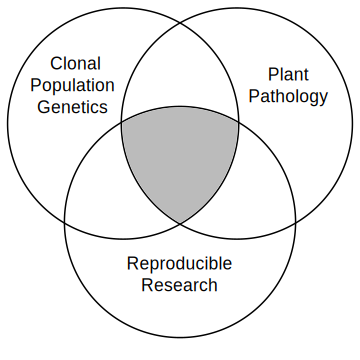
\includegraphics[width=0.5\linewidth]{figure/introduction/dissertation} 
  
  }
  
  \caption[A graphical representation of the three themes governing the work
  presented in this dissertation.]{A graphical representation of the three themes governing the work
  presented in this dissertation.}\label{fig:introduction1}
  \end{figure}
  
  The work presented here offers tools designed to answer questions
  related to clonal population genetics and plant pathology (Fig.
  \ref{fig:introduction1}). In this context, the term `tool' refers to
  software code used to apply mathematical models or theory to population
  genetic data. The merit of this work lies within the context of
  reproducible science, which ensures that the computational environment
  used to create results can be replicated (Buckheit \& Donoho,
  \protect\hyperlink{ref-buckheit1995wavelab}{1995}). The end goal was not
  simply the development of the software, but rather, the development of
  software for the goal of analyzing our own data. Serendipitously, by
  analyzing our own data with this software, we are able to not only
  demonstrate that it can be used, but also demonstrate that an entire
  analysis can be conducted in an open and reproducible manner. We
  demonstrate the usefulness and flexibility of these tools by using them
  to show evidence for multiple introductions in the Curry County, OR
  outbreak of the sudden oak death pathogen, \emph{Phytophthora ramorum}.
  We additionally assess the power of the multilocus linkage
  disequilibrium measure \(\bar{r}_d\) to detect clonal reproduction.
  
  \subsection{Summary of Chapter 2}\label{summary-of-chapter-2}
  
  To address the lack of tools for reproducible research in clonal
  population genetics, we present the software package \emph{poppr} in the
  R computing language (Kamvar et al.,
  \protect\hyperlink{ref-kamvar2014poppr}{2014}\protect\hyperlink{ref-kamvar2014poppr}{b};
  R Core Team, \protect\hyperlink{ref-R2016}{2016}). Previously, tools
  necessary for the analysis of clonal populations were available in
  several stand-alone software programs, each requiring different data
  input formats. Moreover, each program had different levels of
  documentation and limited support for all computing platforms. The
  novelty of \emph{poppr} was to introduce indices of multilocus genotypic
  diversity, the index of association, and a fast implementation of
  Bruvo's genetic distance, and clone-correction over unlimited levels of
  user-specified population hierarchies (Agapow \& Burt,
  \protect\hyperlink{ref-Agapow_2001}{2001}; Arnaud-Hanod et al.,
  \protect\hyperlink{ref-arnaud2007standardizing}{2007}; Bruvo et al.,
  \protect\hyperlink{ref-bruvo2004simple}{2004}). Because this was
  implemented in R these analyses can be performed in a reproducible
  manner on all computing platforms.
  
  \subsection{Summary of Chapter 3}\label{summary-of-chapter-3}
  
  The initial implementation of \emph{poppr} contained basic tools for
  analysis of clonal populations (Kamvar et al.,
  \protect\hyperlink{ref-kamvar2014poppr}{2014}\protect\hyperlink{ref-kamvar2014poppr}{b}),
  but lacked tools for custom definitions of multilocus genotypes and
  performed poorly with genomic-scale data. Chapter 3 introduces an
  updated and improved \emph{poppr} version 2.0. With high throughput
  sequencing (HTS) data, the amount of missing data and genotyping error
  increases, and the definition of a multilocus genotype becomes unclear.
  Moreover, the calculation of the index of association scales poorly with
  an increase in the number of loci. To address these limitations, we
  improved \emph{poppr} with new functionalities to define multilocus
  genotypes based on genetic distance and calculate the index of
  association over random samples or windows of SNP loci.
  
  \subsection{Summary of Chapter 4}\label{summary-of-chapter-4}
  
  A newly-emerged disease of oak---called Sudden Oak Death---spread from
  California to the Southwest corner of Oregon in 2001. Because of intense
  management strategies, the epidemic was largely contained to Curry
  county for the next 15 years. In 2011, an isolated patch of disease
  appeared in Cape Sebastian, 12 miles from the nearest infected site.
  With microsatellite genotyping performed across 2 labs and 15 years, we
  sought to describe the spread of the epidemic in a population genetic
  context and ask the question of whether or not there was evidence for
  more than one introduction event. This work provided evidence supporting
  at least two introductions to Curry county forests. All the analyses
  were performed in an open-source and reproducible manner using R.
  
  \subsection{Summary of Chapter 5}\label{summary-of-chapter-5}
  
  The index of association is a measure of multilocus linkage
  disequilibrium, that is, a correlation coefficient across multiple loci.
  In sexual populations, loci are randomly assorting due to recombination,
  resulting in a near-zero value of the index of association. In clonal
  populations, recombination is non-existent, meaning that loci are passed
  from parent to offspring in a non-independent fashion, resulting in a
  significantly non-zero value of the index of association. De Meeûs \&
  Balloux (\protect\hyperlink{ref-de2004clonal}{2004}) demonstrated that
  this index shows high variance with low levels of sexual reproduction,
  but due to limitations in software, they were not able to perform power
  analyses. We used \emph{poppr} to investigate the power of the index of
  association to detect sexual reproduction in simulated data sets
  generated with microsatellite and genomic markers. This chapter provides
  novel insights on the power, sensitivity, and scope of the index of
  association.
  
  \chapter{\texorpdfstring{\emph{Poppr}: an R Package For Genetic Analysis
  of Populations With Clonal, Partially Clonal, and/or Sexual
  Reproduction}{Poppr: an R Package For Genetic Analysis of Populations With Clonal, Partially Clonal, and/or Sexual Reproduction}}\label{poppr-an-r-package-for-genetic-analysis-of-populations-with-clonal-partially-clonal-andor-sexual-reproduction}
  
  \singlespacing
  
  \begin{center}
  
  Zhian N. Kamvar, Javier F. Tabima, and Niklaus J. Grünwald
  
  
  
  \end{center}\vspace*{\fill}
  
  Journal: \textbf{PeerJ}
  
  PO Box 614, Corte Madera, CA 94976, USA
  
  Published 2014-03-04, Issue: \textbf{2}:e281, DOI:
  \href{https://dx.doi.org/10.7717/peerj.281}{10.7717/peerj.281}
  
  \doublespacing
  \newpage
  
  \section{Abstract}\label{abstract}
  
  Many microbial, fungal, or oomcyete populations violate assumptions for
  population genetic analysis because these populations are clonal,
  admixed, partially clonal, and/or sexual. Furthermore, few tools exist
  that are specifically designed for analyzing data from clonal
  populations, making analysis difficult and haphazard. We developed the R
  package poppr providing unique tools for analysis of data from admixed,
  clonal, mixed, and/or sexual populations. Currently, poppr can be used
  for dominant/codominant and haploid/diploid genetic data. Data can be
  imported from several formats including GenAlEx formatted text files and
  can be analyzed on a user-defined hierarchy that includes unlimited
  levels of subpopulation structure and clone censoring. New functions
  include calculation of Bruvo's distance for microsatellites,
  batch-analysis of the index of association with several indices of
  genotypic diversity, and graphing including dendrograms with bootstrap
  support and minimum spanning networks. While functions for genotypic
  diversity and clone censoring are specific for clonal populations,
  several functions found in poppr are also valuable to analysis of any
  populations. A manual with documentation and examples is provided. Poppr
  is open source and major releases are available on CRAN:
  \url{http://cran.r-project.org/package=poppr}. More supporting
  documentation and tutorials can be found under `resources' at:
  \url{http://grunwaldlab.cgrb.oregonstate.edu/}.
  
  \section{Introduction}\label{introduction-1}
  
  The Wright-Fisher model of populations is one of the oldest models
  utilized in population genetic theory. Populations in this model are
  characterized as having non-overlapping generations with a constant size
  free from any selective pressures (Hartl \& Clark,
  \protect\hyperlink{ref-hartl1997principles}{2007}; Nielsen \& Slatkin,
  \protect\hyperlink{ref-nielsen2013introduction}{2013}; Weir \&
  Cockerham, \protect\hyperlink{ref-weir1996genetic}{1996}). Conceptually,
  these populations are represented as pools of alleles that are
  independently assorting where random mating is approximated by randomly
  sampling alleles with replacement from one generation to the next.
  Assumptions of this model, or related models, are implicitly assumed for
  common population genetic analysis tools. In clonal populations,
  however, alleles are not independently passed on from one generation to
  the next, and these assumptions are violated. Classical textbooks on
  population genetics do not provide much guidance on how to analyze
  clonal or mixed clonal and sexual populations. In reality, many
  populations are not strictly clonal or sexual, but can range from
  completely sexual to completely clonal and this is commonly observed for
  fungal, oomycete, or microbial populations (Anderson \& Kohn,
  \protect\hyperlink{ref-anderson1995clonality}{1995}; Milgroom,
  \protect\hyperlink{ref-milgroom1996recombination}{1996}). Currently,
  analysis of these populations is not straightforward as we lack the
  sophisticated tools and methods developed for model populations that are
  typically either haploid or diploid (Grünwald \& Goss,
  \protect\hyperlink{ref-grunwald2011evolution}{2011}).
  
  Inferring population structure with many commonly used model-based
  clustering approaches such as the program \textsc{ Structure} (Pritchard
  et al., \protect\hyperlink{ref-pritchard2000inference}{2000}) is
  inherently problematic for clonal populations. These approaches cannot
  be used as clonal populations violate basic assumptions of panmixia and
  Hardy-Weinberg equilibrium. Thus, model free methods such as those
  relying on k-means clustering, dendrograms including bootstrap support
  for clades, or minimum spanning networks are more appropriate (Cooke et
  al., \protect\hyperlink{ref-cooke2012genome}{2012}; Goss et al.,
  \protect\hyperlink{ref-goss2009population}{2009}; Mascheretti et al.,
  \protect\hyperlink{ref-mascheretti2008reconstruction}{2008}).
  Furthermore, analysis of mixed or clonal populations traditionally
  relies on calculation of diversity of genotypes observed and analysis of
  clone-censored versus non-censored populations (Grünwald \& Hoheisel,
  \protect\hyperlink{ref-grunwald2006hierarchical}{2006}; McDonald,
  \protect\hyperlink{ref-mcdonald1997population}{1997}; Milgroom,
  \protect\hyperlink{ref-milgroom1996recombination}{1996}). Clone
  censoring involves reduction of any population sample to a single
  observation for each multilocus genotype (MLG) in a population thereby
  approximating panmictic populations and removing the effect of genetic
  linkage (Milgroom,
  \protect\hyperlink{ref-milgroom1996recombination}{1996}). Analysis of
  diversity, in turn, involves calculation of the number of genotypes
  observed (richness), diversity, and evenness (Grünwald et al.,
  \protect\hyperlink{ref-grunwald2003analysis}{2003}). Typical measures of
  genotypic diversity are borrowed from ecology and use either the
  Shannon-Wiener or Stoddart and Taylor index (Grünwald et al.,
  \protect\hyperlink{ref-grunwald2003analysis}{2003}; Shannon,
  \protect\hyperlink{ref-shannon2001mathematical}{1948}; Stoddart \&
  Taylor, \protect\hyperlink{ref-stoddart1988genotypic}{1988}).
  
  A critical aspect of analyzing clonal or mixed populations is testing a
  null hypothesis of panmixia (Milgroom,
  \protect\hyperlink{ref-milgroom1996recombination}{1996}). Testing of
  this hypothesis for potentially clonal populations typically relies on
  assessment of linkage disequilibrium among loci (Milgroom,
  \protect\hyperlink{ref-milgroom1996recombination}{1996}). This is
  achieved via calculation of the index of association or related indices
  in combination with resampling of the data to obtain a null distribution
  for the expectation of random mating (Brown et al.,
  \protect\hyperlink{ref-brown1980multilocus}{1980}; Burt et al.,
  \protect\hyperlink{ref-burt1996molecular}{1996}; Milgroom,
  \protect\hyperlink{ref-milgroom1996recombination}{1996}; Smith et al.,
  \protect\hyperlink{ref-smith1993how}{1993}). These approaches have, for
  example, been applied to \emph{Pyrenophora teres} (Peever \& Milgroom,
  \protect\hyperlink{ref-peever1994genetic}{1994}) and \emph{Aphanomyces
  euteiches} (Grünwald \& Hoheisel,
  \protect\hyperlink{ref-grunwald2006hierarchical}{2006}) and are
  routinely used in the analyses of clonal populations although they are
  not easily calculated given available software including
  \textsc{Multilocus}, which is no longer supported, and \textsc{LIAN},
  which only works for haploids (Agapow \& Burt,
  \protect\hyperlink{ref-Agapow_2001}{2001}; Haubold \& Hudson,
  \protect\hyperlink{ref-Haubold:2000}{2000}).
  
  Hierarchical sampling adds another layer of complexity to analysis of
  clonal populations. With microbial populations, the geographic structure
  of each population is not entirely clear, and it is often important to
  sample temporally to see if clones persist over time (Grünwald \&
  Hoheisel, \protect\hyperlink{ref-grunwald2006hierarchical}{2006}). A
  common approach when faced with multiple levels of sampling is to create
  a separate data set for each level or combination of levels and to
  analyze them separately. However, the number of data sets undergo a
  factorial increase with each hierarchical level, therefore increasing
  the chances of human error in data reformatting or analysis. Thus, tools
  are needed for analysis of population data across hierarchies or subsets
  of data.
  
  Here, we introduce the R package \emph{poppr} that is specifically
  designed for analysis of populations that are clonal, admixed and/or
  sexual. \emph{Poppr} complements and builds on previously existing R
  packages including \emph{adegenet} and \emph{vegan} (Jombart,
  \protect\hyperlink{ref-Jombart_2008}{2008}; Jombart \& Ahmed,
  \protect\hyperlink{ref-jombart2011adegenet}{2011}; Oksanen et al.,
  \protect\hyperlink{ref-oksanen2013vegan}{2013}) while implementing tools
  novel to R significantly facilitating data import, population genetic
  analyses, and graphing of clonal or partially clonal populations. These
  tools include among others: analysis across hierarchies of populations,
  subsetting of populations, clone-censoring, Bruvo's genetic distance
  Bruvo et al. (\protect\hyperlink{ref-bruvo2004simple}{2004}), the index
  of association and related statistics (Brown et al.,
  \protect\hyperlink{ref-brown1980multilocus}{1980}; Smith et al.,
  \protect\hyperlink{ref-smith1993how}{1993}), and bootstrap support for
  trees based on Bruvo's distance. By providing a centralized suite of
  tools appropriate for many data types, this package represents a novel
  and useful resource specifically tailored for analysis of clonal
  populations.
  
  \section{Materials and Methods}\label{materials-and-methods}
  
  \subsection{Data import}\label{data-import}
  
  \emph{Poppr} allows import of data in several formats for
  dominant/codominant, haploid/diploid and geographic data. The R package
  \emph{adegenet}, that defines the \texttt{genind} data structure that
  \emph{poppr} utilizes, allows support for importing data natively from
  \textsc{Structure, Genetix, Genepop}, and \textsc{Fstat}. While these
  formats are very common and widely supported, these do not allow for
  import of geographic and/or regional data. Furthermore, \emph{adegenet}
  will only handle diploids with this format, though manual import is
  possible. To aid in importing data, \emph{poppr} has newly added the
  function \texttt{read.genalex()}, to read data from \emph{GenAlEx}
  formatted text files into the \texttt{genind} data object of the package
  \emph{adegenet} (Jombart, \protect\hyperlink{ref-Jombart_2008}{2008};
  Jombart \& Ahmed, \protect\hyperlink{ref-jombart2011adegenet}{2011};
  Peakall \& Smouse, \protect\hyperlink{ref-Peakall:2006}{2006}).
  \emph{GenAlEx} is a popular add-in for \textsc{Microsoft Excel} that can
  handle data including codominant/dominant and haploid/diploid markers as
  well as geographic and regional data. This function further facilitates
  the import of haploid, geographic, and regional data.
  
  Transferring data to new formats and manipulating data by hand, such as
  collapsing data into clones or subsetting data into different
  hierarchical levels, is tedious, creates redundancy, and can result in
  lost or misrepresented data. \emph{Poppr} includes tools to automate
  such repetitive tasks. Many currently available data formats and
  software implementations allow analysis of only one or two levels of a
  population hierarchy. With \emph{poppr} the user can import a single
  data set with an unlimited number of hierarchical levels. This is
  achieved by having the user combine the levels using a common delimiter
  (e.g. ``Year\_Country\_City''). These combined levels are then used as
  the defining population factor in the input file and can easily be
  manipulated within R.
  
  \subsection{Data analysis}\label{data-analysis}
  
  Once data is imported into R, the user can dynamically access and
  manipulate the population hierarchy with the function
  \texttt{splitcombine()}, subset the data set by population with
  \texttt{popsub()}, and check for cloned multilocus genotypes using
  \texttt{mlg()}. For data sets that include clones, the \emph{poppr}
  function \texttt{clonecorrect()} will censor exact clones with respect
  to any level of a population hierarchy by creating a new data set that
  includes only unique multilocus genotypes (MLGs) per population. A full
  list of functions available in \emph{poppr} is provided in table
  \ref{tab:poppr1}.
  
  \begin{sidewaystable}[ph!]
  \caption{List of functions found in \textit{poppr} and short descriptions.}
  \label{tab:poppr1}
  \begin{tabular}{ll}
  \hline
  Function & Description \\ 
  \hline
  \textbf{Import/Export} & \\
  \texttt{getfile} & Provides a quick GUI to grab files for import \\
  \texttt{read.genalex} & Read \textit{GenAlEx} formatted csv files to a genind object \\
  \texttt{genind2genalex} & Converts genind objects to \textit{GenAlEx} formatted csv files \\
  \hline
  \textbf{Manipulation} & \\
  \texttt{missingno} & Handles missing data \\
  \texttt{clonecorrect} & Clone censors at a specified population hierarchy \\
  \texttt{informloci} & Detects and removes phylogenetically uninformative loci. \\
  \texttt{popsub} & Subsets genind objects by population \\
  \texttt{shufflepop} & Shuffles genotypes at each locus using four different algorithms (details in table \ref{tab:poppr3}) \\
  \texttt{splitcombine} & Manipulates population hierarchy \\ 
  \hline
  \textbf{Analysis} & \\
  \texttt{bruvo.boot} & Produces dendrograms with bootstrap support based on Bruvo's distance \\
  \texttt{bruvo.dist} & Calculates Bruvo's distance \\
  \texttt{diss.dist} & Calculates the percent allelic dissimilarity \\
  \texttt{ia} & Calculates the index of association \\
  \texttt{mlg} & Calculates the number of multilocus genotypes \\
  \texttt{mlg.crosspop} & Finds all multilocus genotypes that cross populations \\
  \texttt{mlg.table} & Returns a table of populations by multilocus genotypes \\
  \texttt{mlg.vector} & Returns a vector of a numeric multilocus genotype assignment for each individual \\
  \texttt{poppr} & Returns a diversity table by population \\
  \texttt{poppr.all} & Returns a diversity table by population for all compatible files specified \\
  \hline
  \textbf{Visualization} & \\
  \texttt{greycurve} & Helper to determine appropriate parameters for adjusting the grey level for msn functions \\
  \texttt{bruvo.msn} & Produces minimum spanning networks based off Bruvo's distance colored by population \\
  \texttt{poppr.msn} & Produces a minimum spanning network for any pairwise distance matrix related to the data \\
  \hline
  
  \end{tabular}
  \end{sidewaystable}
  
  Typical analyses in \emph{poppr} start with summary statistics for
  diversity, rarefaction, evenness, MLG counts, and calculation of
  distance measures such as Bruvo's distance, providing a suitable
  stepwise mutation model appropriate for microsatellite markers (Bruvo et
  al., \protect\hyperlink{ref-bruvo2004simple}{2004}). \emph{Poppr} will
  define MLGs in your data set, show where they cross populations, and can
  produce graphs and tables of MLGs by population that can be used for
  further analysis with the R package \emph{vegan} Oksanen et al.
  (\protect\hyperlink{ref-oksanen2013vegan}{2013}). Many of the diversity
  indices calculated by the \emph{vegan} function \texttt{diversity()} are
  useful in analyzing the diversity of partially clonal populations. For
  this reason, \emph{poppr} features a quick summary table (Table
  \ref{tab:poppr2}) that incorporates these indices along with the index
  of association, \(I_A\) (Brown et al.,
  \protect\hyperlink{ref-brown1980multilocus}{1980}; Smith et al.,
  \protect\hyperlink{ref-smith1993how}{1993}), and its standardized form,
  \(\bar{r}_d\), which accounts for the number of loci sampled (Agapow \&
  Burt, \protect\hyperlink{ref-Agapow_2001}{2001}). Both measures of
  association can detect signatures of multilocus linkage and values
  significantly departing from the null model of no linkage among markers
  are detected via permutation analysis utilizing one of four algorithms
  described in table \ref{tab:poppr3} (Agapow \& Burt,
  \protect\hyperlink{ref-Agapow_2001}{2001}). The user can specify the
  number of samples taken from the observed data set to obtain the null
  distribution expected for a randomly mating population. Detailed
  examples of these analyses can be found in the \emph{poppr} manual.
  
  \begin{sidewaystable}[ph!]
  \centering
  \caption[Summary table shown as it would appear in the R console produced by the poppr() function.]{
  Summary table shown as it would appear in the R console produced by the
  \texttt{poppr()} function with 999 permutations to calculate \(I_A\) and
  \(\bar{r}_d\) p-values from the \texttt{Aeut} data set in \textit{poppr}
  from (Grünwald et al.,
  \protect\hyperlink{ref-grunwald2003analysis}{2003}). \texttt{N}: census
  size, \texttt{MLG}: multilocus genotypes, \texttt{eMLG}: expected MLG
  based on rarefaction, \texttt{SE}: standard error from rarefaction,
  \texttt{H}: Shannon-Wiener Index, \texttt{G}: Stoddart and Taylor's
  Index, \texttt{Hexp}: Nei 1978 Expected Heterozygosity, \texttt{E.5}:
  Evenness (\(E_5\)), \texttt{Ia}: \(I_A\), \texttt{p.Ia}: p-value for
  \(I_A\), \texttt{rbarD}: \(\bar{r}_d\), \texttt{p.rD}: p-value for
  \(\bar{r}_d\). Table was obtained with the following code:
  \texttt{library(poppr);\ data(Aeut);\ poppr(Aeut,\ sample\ =\ 999)}.} 
  \label{tab:poppr2}
  \begin{tabular}{rrrrrrrrrrrrr}
    \toprule
  \texttt{Pop} & \texttt{N} & \texttt{MLG} & \texttt{eMLG} & \texttt{SE} & \texttt{H} & \texttt{G} & \texttt{Hexp} & \texttt{E.5} & \texttt{Ia} & \texttt{p.Ia} & \texttt{rbarD} & \texttt{p.rD} \\ 
   \texttt{Athena} &  97 &  70 & 65.98 & 1.25 & 4.06 & 42.19 & 0.99 & 0.72 & 2.91 & 0.00 & 0.07 & 0.00 \\ 
    \texttt{Mt. Vernon} &  90 &  50 & 50.00 & 0.00 & 3.67 & 28.72 & 0.98 & 0.73 & 13.30 & 0.00 & 0.28 & 0.00 \\ 
    \texttt{Total} & 187 & 119 & 68.45 & 2.99 & 4.56 & 68.97 & 0.99 & 0.72 & 14.37 & 0.00 & 0.27 & 0.00 \\ 
     \bottomrule
  \end{tabular}
  \end{sidewaystable}
  
  \begin{sidewaystable}[ph!]
  \caption{Permutation algorithms in \textit{poppr} implemented in the calculation of $I_A$ and $\bar{r}_d$ p-values, iterated over all loci independently.}
  \label{tab:poppr3}
  \begin{tabular}{clccc}
  \hline
  \textbf{Method} & \textbf{Name} & \textbf{Units Sampled} & \textbf{With Replacement} & \textbf{Weight} \\
  \hline
  1 & \texttt{permutation} & alleles & No & - \\
  2 & \texttt{parametric bootstrap} & alleles & Yes & allele frequencies \\
  3 & \texttt{non-parametric bootstrap} & alleles & Yes & equal \\
  4 & \texttt{multilocus} & genotypes & No & - \\
  \hline
  \end{tabular}
  
  \end{sidewaystable}
  
  \subsection{Visualizations}\label{visualizations}
  
  \emph{Poppr} generates bar charts of MLG counts found within each
  population of your data set (Fig. \ref{fig:poppr1}). Histograms with rug
  plots for \(I_A\) and \(\bar{r}_d\) allow visual assessment of the
  quality of the distribution derived from resampling to see if a higher
  number of replications are necessary (Fig. \ref{fig:poppr2}).
  \emph{Poppr} automatically produces custom minimum spanning networks for
  Bruvo's or other distances using Prim's algorithm, as implemented in the
  package \emph{igraph} Csardi \& Nepusz
  (\protect\hyperlink{ref-csardi2006igraph}{2006}), with the functions
  \texttt{bruvo.msn()} for Bruvo's distance (Fig. \ref{fig:poppr3}) and
  \texttt{poppr.msn()} for any distance matrix. The combination of data
  structures from \emph{adegenet} and \emph{igraph} allow graphing that is
  color coded by population with vertices grouped by MLG (Csardi \&
  Nepusz, \protect\hyperlink{ref-csardi2006igraph}{2006}; Jombart,
  \protect\hyperlink{ref-Jombart_2008}{2008}; Jombart \& Ahmed,
  \protect\hyperlink{ref-jombart2011adegenet}{2011}). \emph{Poppr} also
  includes visualization of dendrograms using UPGMA Schliep
  (\protect\hyperlink{ref-phangorn}{2011}) and Neighbor-Joining Paradis et
  al. (\protect\hyperlink{ref-paradis2004ape}{2004}) algorithms with
  bootstrap support for Bruvo's distance using the function
  \texttt{bruvo.boot()} (Fig. \ref{fig:poppr4}). Neither graphing of
  minimum spanning networks or dendrograms with bootstrap support are
  currently possible for populations in any other R packages.
  
  \begin{figure}
  
  {\centering \includegraphics[width=0.8\linewidth]{figure/poppr/Finland} 
  
  }
  
  \caption[Distribution of 12 multilocus genotypes from the \texttt{Finland}
  population of the \texttt{H3N2} SNP data set (Jombart,
  \protect\hyperlink{ref-Jombart_2008}{2008})]{Distribution of 12 multilocus genotypes from the \texttt{Finland}
  population of the \texttt{H3N2} SNP data set (Jombart,
  \protect\hyperlink{ref-Jombart_2008}{2008})}\label{fig:poppr1}
  \end{figure}
  
  \newpage
  
  \begin{figure}
  
  {\centering \includegraphics[width=0.7\linewidth]{figure/poppr/nancy_5} 
  
  }
  
  \caption[Visualizations of tests for linkage disequilibrium.]{Visualizations of tests for linkage disequilibrium, where observed
  values (blue dashed lines) of \(I_A\) and \(\bar{r}_d\) are compared to
  histograms showing results of 999 permutations using method 1 in table
  \ref{tab:poppr1}. Results are shown for the sexual population \texttt{5}
  of the \texttt{nancycats} data set (Jombart,
  \protect\hyperlink{ref-Jombart_2008}{2008}) (a) and for the clonal
  \texttt{Athena} population of the \texttt{Aeut} data set (Grünwald et
  al., \protect\hyperlink{ref-grunwald2003analysis}{2003}) (b).}\label{fig:poppr2}
  \end{figure}
  
  \newpage
  
  \begin{figure}
  
  {\centering \includegraphics[width=0.8\linewidth]{figure/poppr/bruvo_color} 
  
  }
  
  \caption[Example minimum spanning network using Bruvo's distance on a simulated
  partially clonal data set with 50 individuals genotyped over 10 microsatellite
  loci.]{Example minimum spanning network using Bruvo's distance on a simulated
  partially clonal data set with 50 individuals genotyped over 10
  microsatellite loci produced with the software SimuPOP v.1.0.8 (Peng \&
  Amos, \protect\hyperlink{ref-peng2008forward}{2008}). Each node
  represents a unique multilocus genotype. Node shading (colors) represent
  population membership, while edge widths and shading represent
  relatedness. Edge length is arbitrary.}\label{fig:poppr3}
  \end{figure}
  
  \newpage
  
  \begin{figure}
  
  {\centering \includegraphics[width=0.8\linewidth]{figure/poppr/nancy9-boot-redo} 
  
  }
  
  \caption[UPGMA tree produced from Bruvo's distance with 1000 bootstrap
  replicates.]{UPGMA tree produced from Bruvo's distance with 1000 bootstrap replicates
  (node values greater than 50\% are shown). Data from population
  \texttt{9} of the \texttt{nancycats} data set (Jombart,
  \protect\hyperlink{ref-Jombart_2008}{2008})}\label{fig:poppr4}
  \end{figure}
  
  \subsection{Performance}\label{performance}
  
  Most of the functions in \emph{Poppr} were written and optimized for
  performance in R and are available for inspection and/or download at
  \url{https://github.com/grunwaldlab/poppr}. Algorithms of
  \(\geq O(n^2)\) complexity were written in the byte-compiled C language
  to optimize runtime performance.
  
  For comparisons of \(I_A\) and Bruvo's distance, we utilized the data
  set `nancycats' (237 diploid individuals genotyped at nine
  microsatellite loci) from the \emph{adegenet} package. Calculations were
  run independently 10 times and then averaged. Bruvo's distance was
  calculated on a machine with OSX 10.8.4 and a 2.9 GHz intel processor.
  The \(I_A\) and \(\bar{r}_d\) calculations were performed on a machine
  with OSX 10.5.8 and a 2.4 GHz intel processor due to the inability of
  the software \textsc{multilocus} to work on any later version of OSX.
  
  \section{\texorpdfstring{Citation of methods implemented in
  \emph{poppr}}{Citation of methods implemented in poppr}}\label{citation-of-methods-implemented-in-poppr}
  
  Several of the methods implemented in \emph{poppr} are described
  elsewhere. Users should refer to the original publications for
  interpretations and citation. See table \ref{tab:poppr4} for a full list
  of citations. As with any R package, users should always cite the R Core
  Team (R Core Team, \protect\hyperlink{ref-R2013}{2013}).
  
  \begin{longtable}[h!]{@{}lcr@{}}
  
  \caption{\label{tab:poppr4} Citation of methods and indices implemented in \emph{poppr}}\tabularnewline
  
  \textbf{Method/Index} & \textbf{Citation} & \textbf{Function(s) in \emph{poppr}}\tabularnewline
  \midrule
  \endfirsthead
  \multicolumn{3}{c}%
  {{\tablename\ \thetable{} -- continued from previous page}} \\
  \textbf{Method/Index} & \textbf{Citation} & \textbf{Function(s) in \emph{poppr}}\tabularnewline
  \endhead
  
  \multicolumn{3}{r}{\textbf{Continued on next page...}} \\
  \endfoot
  
  \endlastfoot
  
  Expected MLG  & (Hurlbert, \protect\hyperlink{ref-hurlbert1971nonconcept}{1971}), & \texttt{poppr()}\tabularnewline
  (rarefaction) & (Heck et al., \protect\hyperlink{ref-heck1975explicit}{1975}) (for std. err.) & \tabularnewline
  \hline
  \(H\) & (Shannon, \protect\hyperlink{ref-shannon2001mathematical}{1948}) & \texttt{poppr()}\tabularnewline
  \hline
  \(G\) & (Stoddart \& Taylor,
  \protect\hyperlink{ref-stoddart1988genotypic}{1988}) & \texttt{poppr()}\tabularnewline
  \hline
  \(H_{exp}\) & (Nei, \protect\hyperlink{ref-Nei:1978}{1978}) & \texttt{poppr()}\tabularnewline
  \hline
  \(E_{5}\) & (Grünwald \& Hoheisel,
  \protect\hyperlink{ref-grunwald2006hierarchical}{2006}), & \texttt{poppr()}\tabularnewline
   & (Ludwig \& Reynolds,
  \protect\hyperlink{ref-ludwig1988statistical}{1988}), & \tabularnewline
   & (Pielou, \protect\hyperlink{ref-pielou1975ecological}{1975}) & \tabularnewline
  \hline
  \(I_A\) & (Brown et al., \protect\hyperlink{ref-brown1980multilocus}{1980}), & \texttt{ia()}\tabularnewline 
   & (Smith et al., \protect\hyperlink{ref-smith1993how}{1993}) & \texttt{poppr()}\tabularnewline
  \hline
  \(\bar{r}_d\) &  (Agapow \& Burt, \protect\hyperlink{ref-Agapow_2001}{2001}) & \texttt{ia()}\tabularnewline 
  & & \texttt{poppr()}\tabularnewline
  \hline
  Clone correction & (Grünwald \& Hoheisel,
  \protect\hyperlink{ref-grunwald2006hierarchical}{2006}), & \texttt{clonecorrect()}\tabularnewline 
   & (Grünwald et al., \protect\hyperlink{ref-grunwald2003analysis}{2003}), & \texttt{poppr()}\tabularnewline
   & (Milgroom, \protect\hyperlink{ref-milgroom1996recombination}{1996}) & \tabularnewline
  \hline
  Minimum Spanning & (Csardi \& Nepusz, \protect\hyperlink{ref-csardi2006igraph}{2006}) & \texttt{poppr.msn()}\tabularnewline 
  Networks & & \texttt{bruvo.msn()}\tabularnewline
  \hline
  Bruvo's Distance & (Bruvo et al., \protect\hyperlink{ref-bruvo2004simple}{2004}) & \texttt{bruvo.dist()}\tabularnewline 
  & & \texttt{bruvo.msn()}\tabularnewline 
  & & \texttt{bruvo.boot()}\tabularnewline
  \hline
  Bootstrapping & (Paradis et al., \protect\hyperlink{ref-paradis2004ape}{2004}) & \texttt{bruvo.boot()}\tabularnewline 
  \hline
  Neighbor Joining & (Paradis et al., \protect\hyperlink{ref-paradis2004ape}{2004}) & \texttt{bruvo.boot()}\tabularnewline
  \hline
  UPGMA & (Schliep, \protect\hyperlink{ref-phangorn}{2011}) & \texttt{bruvo.boot()}\tabularnewline 
  \bottomrule
  \end{longtable}
  
  \section{Results and Discussion}\label{results-and-discussion}
  
  \emph{Poppr} provides significant, convenient tools for analysis of
  clonal and partially clonal populations available in one environment on
  all major operating systems. The ability to analyze data for multiple
  populations across a user-defined hierarchy and clone-censoring provide
  novel functionality in R. Combined with R's graphing abilities,
  publication-ready figures are thus obtained conveniently.
  
  \subsection{New functionalities}\label{new-functionalities}
  
  \begin{longtable}[]{@{}lccccc@{}}
  \caption{\label{tab:poppr5} Comparison of programs that calculate
  \(I_A\)}\tabularnewline
  \toprule
  & \textbf{Haploids} & \textbf{Diploids} & \(\bar{r}_d\) & \textbf{All
  Platforms} & \textbf{Batch Analysis}\tabularnewline
  \midrule
  \endfirsthead
  \toprule
  & \textbf{Haploids} & \textbf{Diploids} & \(\bar{r}_d\) & \textbf{All
  Platforms} & \textbf{Batch Analysis}\tabularnewline
  \midrule
  \endhead
  \emph{poppr} & Yes & Yes & Yes & Yes & Yes\tabularnewline
  \emph{LIAN} & Yes & No & No & Yes & Yes\tabularnewline
  \emph{multilocus} & Yes & Yes & Yes & No & No\tabularnewline
  \bottomrule
  \end{longtable}
  
  \emph{Poppr} implements several new functionalities. As of this writing,
  aside from \emph{poppr}, there exist two programs that calculate
  \(I_A\): \textsc{LIAN} (Haubold \& Hudson,
  \protect\hyperlink{ref-Haubold:2000}{2000}) and \textsc{multilocus}
  (Agapow \& Burt, \protect\hyperlink{ref-Agapow_2001}{2001}).
  \textsc{LIAN} can calculate \(I_A\) for haploid data and is only
  available online or for *nix systems with a C compiler such as OSX and
  Linux (Haubold \& Hudson, \protect\hyperlink{ref-Haubold:2000}{2000}).
  \textsc{Multilocus} implemented \(\bar{r}_d\), a novel correction for
  \(I_A\), but is no longer supported (Agapow \& Burt,
  \protect\hyperlink{ref-Agapow_2001}{2001}). \textsc{Multilocus} will
  only calculate index values for one data set at a time and \textsc{LIAN}
  requires the user to structure the data set with populations in
  contiguous blocks to analyze multiple populations within a single file.
  Thus \emph{poppr} provides significant improvements for calculation of
  linkage disequilibrium, and handles both haploid and diploid data, works
  on all major operating systems, and is capable of batch analysis of
  multiple files and multiple populations defined within a file including
  the possibility of clone correction and sub-setting. A comparison of the
  capabilities of these programs are summarized in Table \ref{tab:poppr5}.
  
  To test significance for \(I_A\) and \(\bar{r}_d\), \emph{poppr} offers
  four permutation algorithms. Each one will randomly shuffle data at each
  locus, effectively unlinking the loci. The algorithm previously utilized
  by \textsc{mutlilocus} is included. The \textsc{multilocus}-style
  algorithm shuffles genotypes, maintaining the associations between
  alleles at each locus (Agapow \& Burt,
  \protect\hyperlink{ref-Agapow_2001}{2001}). More appropriately, alleles
  are expected to assort independently in panmictic populations.
  \emph{Poppr} thus provides three new algorithms for permutation that
  allow for independent allele assortment at each locus. The default
  algorithm permutes the alleles at each locus and the remaining two will
  randomly sample alleles from a multinomial distribution parametrically
  and non-parametrically (Weir \& Cockerham,
  \protect\hyperlink{ref-weir1996genetic}{1996}). Details of these
  algorithms are presented in table \ref{tab:poppr3}. Because the index of
  association is calculated using a binary measure of dissimilarity, we
  have also made this available as a distance measure called
  \texttt{diss.dist()}. This pairwise distance is based on the percent
  allelic differences.
  
  \emph{Poppr} also newly implements Bruvo's genetic distance that
  utilizes a stepwise mutation model appropriate for microsatellite data
  (Bruvo et al., \protect\hyperlink{ref-bruvo2004simple}{2004}). While
  this distance is implemented in the program \textsc{ GenoDive} Meirmans
  \& Van Tienderen (\protect\hyperlink{ref-meirmans2004genotype}{2004})
  and the R package \emph{polysat} Clark \& Jasieniuk
  (\protect\hyperlink{ref-polysat}{2011}), there are a few caveats with
  these two implementations. \textsc{GenoDive} is closed-source, and only
  implemented in OSX. Both \emph{poppr} and \emph{polysat} are open-source
  and available on all platforms, but \emph{polysat}, being optimized for
  polyploid individuals with ambiguous allelic dosage, is inappropriate
  for analyzing diploids. \emph{Polysat} will collapse homozygous
  individuals into a single allele and attempt to infer the second allelic
  state in comparison with heterozygous individuals. Since haploid and
  diploid individuals show clear allelic dosage, this procedure creates a
  bias misrepresenting the true distance. Not only is \emph{poppr} not
  subject to this bias, but it also newly introduces bootstrap support for
  this distance as shown in Figure \ref{fig:poppr4}.
  
  \subsection{Performance}\label{performance-1}
  
  \begin{longtable}[]{@{}lcc@{}}
  \caption{\label{tab:poppr6} Comparison of performance on one data set of 237
  individuals over nine loci. Each time point represents an average of 10
  independent runs. Calculations of \(I_A\) are based on 100
  permutations.}\tabularnewline
  \toprule
  & \textbf{\(I_A\) (seconds)} & \textbf{Bruvo's distance
  (seconds)}\tabularnewline
  \midrule
  \endfirsthead
  \toprule
  & \textbf{\(I_A\) (seconds)} & \textbf{Bruvo's distance
  (seconds)}\tabularnewline
  \midrule
  \endhead
  \emph{poppr} & 13.4 & 0.3\tabularnewline
  \emph{polysat} & - & 58.3\tabularnewline
  \emph{multilocus} & 547.2 & -\tabularnewline
  \bottomrule
  \end{longtable}
  
  \emph{Poppr} reduces the amount of intermediate files and repetitive
  tasks needed for basic population genetic analyses and implements
  computationally intensive functions, such as Bruvo's distance and the
  index of association in C to improve performance. The \emph{polysat}
  package calculation of Bruvo's distance took 58.3 seconds on average
  whereas \emph{poppr}'s calculation was over 190 times faster, averaging
  0.3 seconds (Table \ref{tab:poppr6}). For calculation of \(I_A\) and
  \(\bar{r}_d\) with 100 permutations and Nei's genotypic diversity (Nei,
  \protect\hyperlink{ref-Nei:1978}{1978}), \textsc{multilocus} required
  around 9.12 minutes on average, as compared to 13.4 seconds with
  \emph{poppr}.
  
  \section{Conclusions}\label{conclusions}
  
  The R package \emph{poppr} provides new functions and tools specifically
  tailored for analysis of data from clonal or partially clonal
  populations. No software currently available provides this set of tools.
  Novel capabilities include analysis across multiple populations at
  multiple levels of hierarchies, clone-censoring, and subsetting. These
  in combination with R's command line interface and scripting
  capabilities makes analyses of these populations more streamlined and
  tractable. By implementing computationally expensive algorithms such as
  Bruvo's distance and \(I_A\) in C, analyses of multiple populations that
  would normally take hours to complete can now be finished in a matter of
  minutes. This allowed us to expand the utility of these measures to
  convenient new graphing abilities such as automatically creating
  dendrograms with bootstrap support for Bruvo's distance and minimum
  spanning networks. While major releases of \emph{poppr} are available on
  CRAN, we are continuing to develop this package to be able to
  efficiently handle genome-sized SNP data. Development versions are
  available on github at \url{https://github.com/grunwaldlab/poppr}.
  
  \section{Acknowledgements}\label{acknowledgements}
  
  The authors would like to thank Sydney Everhart and Corine Schoebel for
  invaluable alpha testing and Paul-Michael Agapow for providing the
  \emph{multilocus} C++ source code for reference. We thank Sydney
  Everhart and Brian Knaus for comments that significantly improved this
  manuscript. Mention of trade names or commercial products in this
  manuscript are solely for the purpose of providing specific information
  and do not imply recommendation or endorsement.
  
  \chapter{Novel R Tools For Analysis of Genome-Wide Population Genetic
  Data With Emphasis on
  Clonality}\label{novel-r-tools-for-analysis-of-genome-wide-population-genetic-data-with-emphasis-on-clonality}
  
  \singlespacing
  
  \begin{center}
  
  Zhian N. Kamvar, Jonah C. Brooks, and Niklaus J. Grünwald
  
  
  
  \end{center}\vspace*{\fill}
  
  Journal: \textbf{Frontiers in Genetics}
  
  EPFL Innovation Park, Building I, CH -- 1015 Lausanne Switzerland
  
  Published 2015-06-10. Issue: \textbf{6}, DOI:
  \href{http://dx.doi.org/10.3389/fgene.2015.00208}{10.3389/fgene.2015.00208}
  
  \doublespacing
  \newpage
  
  \section{Abstract}\label{abstract-1}
  
  To gain a detailed understanding of how plant microbes evolve and adapt
  to hosts, pesticides, and other factors, knowledge of the population
  dynamics and evolutionary history of populations is crucial. Plant
  pathogen populations are often clonal or partially clonal which requires
  different analytical tools. With the advent of high throughput
  sequencing technologies, obtaining genome-wide population genetic data
  has become easier than ever before. We previously contributed the R
  package \emph{poppr} specifically addressing issues with analysis of
  clonal populations. In this paper we provide several significant
  extensions to \emph{poppr} with a focus on large, genome-wide SNP data.
  Specifically, we provide several new functionalities including the new
  function \texttt{mlg.filter} to define clone boundaries allowing for
  inspection and definition of what is a clonal lineage, minimum spanning
  networks with reticulation, a sliding-window analysis of the index of
  association, modular bootstrapping of any genetic distance, and analyses
  across any level of hierarchies.
  
  \section{Introduction}\label{introduction-2}
  
  To paraphrase Dobzhansky, nothing in the field of plant-microbe
  interactions makes sense except in the light of population genetics
  (Dobzhansky, \protect\hyperlink{ref-dobzhansky2013nothing}{1973}).
  Genetic forces such as selection and drift act on alleles in a
  population. Thus, a true understanding of how plant pathogens emerge,
  evolve and adapt to crops, fungicides, or other factors, can only be
  elucidated in the context of population level phenomena given the
  demographic history of populations (Grünwald \& Goss,
  \protect\hyperlink{ref-grunwald2011evolution}{2011}; McDonald \& Linde,
  \protect\hyperlink{ref-Mcdonald2002}{2002}\protect\hyperlink{ref-Mcdonald2002}{b};
  Milgroom et al., \protect\hyperlink{ref-milgroom1989population}{1989}).
  The field of population genetics, in the era of whole genome
  resequencing, provides unprecedented power to describe the evolutionary
  history and population processes that drive coevolution between
  pathogens and hosts. This powerful field thus critically enables
  effective deployment of R genes, design of pathogen informed plant
  resistance breeding programs, and implementation of fungicide rotations
  that minimize emergence of resistance.
  
  Most computational tools for population genetics are based on concepts
  developed for sexual model organisms. Populations that reproduce
  clonally or are polyploid are thus difficult to characterize using
  classical population genetic tools because theoretical assumptions
  underlying the theory are violated. Yet, many plant pathogen populations
  are at least partially clonal if not completely clonal (Anderson \&
  Kohn, \protect\hyperlink{ref-anderson1995clonality}{1995}; Milgroom,
  \protect\hyperlink{ref-milgroom1996recombination}{1996}). Thus,
  development of tools for analysis of clonal or polyploid populations is
  needed.
  
  Genotyping by sequencing and whole genome resequencing provide the
  unprecedented ability to identify thousands of single nucleotide
  polymorphisms (SNPs) in populations (Davey et al.,
  \protect\hyperlink{ref-davey2011genome}{2011}; Elshire et al.,
  \protect\hyperlink{ref-elshire2011robust}{2011}; Luikart et al.,
  \protect\hyperlink{ref-luikart2003power}{2003}). With traditional marker
  data (e.g., SSR, AFLP) a clone was typically defined as a unique
  multilocus genotype (MLG) (Cooke et al.,
  \protect\hyperlink{ref-cooke2012genome}{2012}; Falush et al.,
  \protect\hyperlink{ref-Falush01082003}{2003}; Goss et al.,
  \protect\hyperlink{ref-goss2009population}{2009}; Grünwald \& Hoheisel,
  \protect\hyperlink{ref-grunwald2006hierarchical}{2006}; Taylor \&
  Fisher, \protect\hyperlink{ref-taylor2003fungal}{2003}). Availability of
  large SNP data sets provides new challenges for data analysis. These
  data are based on reduced representation libraries and high throughput
  sequencing with moderate sequencing depth which invariably results in
  substantial missing data, error in SNP calling due to sequencing error,
  lack of read depth or other sources of spurious allele calls
  (Mastretta-Yanes et al.,
  \protect\hyperlink{ref-mastretta2015restriction}{2014}). It is thus not
  clear what a clone is in large SNP data sets and novel tools are
  required for definition of clone boundaries.
  
  The research community using the R statistical and computing language (R
  Core Team, \protect\hyperlink{ref-R}{2015}) has developed a plethora of
  new resources for population genetic analysis. R is particularly
  appealing because all code is open source and functions can be evaluated
  and modified by any user. Recently, we introduced the R package
  \emph{poppr} specifically developed for analysis of clonal populations
  (Kamvar et al.,
  \protect\hyperlink{ref-kamvar2014poppr}{2014}\protect\hyperlink{ref-kamvar2014poppr}{b}).
  \emph{Poppr} previously introduced several novel features including the
  ability to conduct a hierarchical analysis across unlimited hierarchies,
  test for linkage association, graph minimum spanning networks or provide
  bootstrap support for Bruvo's distance in resulting trees. \emph{Poppr}
  has been rapidly adopted and applied to a range of studies including for
  example horizontal transmission in leukemia of clams (Metzger et al.,
  \protect\hyperlink{ref-metzger2015horizontal}{2015}), study of the
  vector-mediated parent-to-offspring transmission in an avian
  malaria-like parasite (Chakarov et al.,
  \protect\hyperlink{ref-chakarov2015apparent}{2015}), and
  characterization of the emergence of the invasive forest pathogen
  \emph{Hymenoscyphus pseudoalbidus} (Gross et al.,
  \protect\hyperlink{ref-gross2014population}{2014}). It has also been
  used to implement real-time, online R based tools for visualizing
  relationships among unknown MLGs in reference databases\\
  (\url{http://phytophthora-id.org/}) (Grünwald et al.,
  \protect\hyperlink{ref-grunwald2011phytophthora}{2011}).
  
  Here, we introduce \emph{poppr} 2.0, which provides a major update to
  \emph{poppr} (Kamvar et al.,
  \protect\hyperlink{ref-kamvar2014poppr}{2014}\protect\hyperlink{ref-kamvar2014poppr}{b})
  including novel tools for analysis of clonal populations specifically
  addressing large SNP data. Significant novel tools include functions for
  calculating clone boundaries and collapsing individuals into clonal
  groups based on a user-specified genetic distance threshold, sliding
  window analyses, genotype accumulation curves, reticulations in minimum
  spanning networks, and bootstrapping for any genetic distance.
  
  \section{Implementations and
  Examples}\label{implementations-and-examples}
  
  \subsection{Clonal identification}\label{clonal-identification}
  
  As highlighted in previous work, clone correction is an important
  component of population genetic analysis of organisms that are known to
  reproduce asexually (Grünwald et al.,
  \protect\hyperlink{ref-grunwald2003analysis}{2003}; Kamvar et al.,
  \protect\hyperlink{ref-kamvar2014poppr}{2014}\protect\hyperlink{ref-kamvar2014poppr}{b};
  Milgroom, \protect\hyperlink{ref-milgroom1996recombination}{1996}). This
  method is a partial correction for bias that affects metrics that rely
  on allele frequencies assuming panmixia and was initially designed for
  data with only a handful of markers. With the advent of large-scale
  sequencing and reduced- representation libraries, it has become easier
  to sequence tens of thousands of markers from hundreds of individuals
  (Davey \& Blaxter, \protect\hyperlink{ref-davey2010rad}{2010}; Davey et
  al., \protect\hyperlink{ref-davey2011genome}{2011}; Elshire et al.,
  \protect\hyperlink{ref-elshire2011robust}{2011}). With this larger
  number of markers, the genetic resolution is much greater, but the
  chance of genotyping error is also greatly increased and missing data is
  frequent (Mastretta-Yanes et al.,
  \protect\hyperlink{ref-mastretta2015restriction}{2014}). Taking this
  fact and occasional somatic mutations into account, it would be
  impossible to separate true clones from independent individuals by just
  comparing what MLGs are different. We introduce a new method for
  collapsing unique multilocus genotypes determined by naive string
  comparison into multilocus lineages utilizing any genetic distance given
  three different clustering algorithms: farthest neighbor, nearest
  neighbor, and UPGMA (average neighbor) (Sokal,
  \protect\hyperlink{ref-sokal1958statistical}{1958}).
  
  These clustering algorithms act on a distance matrix that is either
  provided by the user or generated via a function that will calculate a
  distance from genetic data such as \texttt{bruvo.dist}, which in
  particular applies to any level of ploidy (Bruvo et al.,
  \protect\hyperlink{ref-bruvo2004simple}{2004}). All algorithms have been
  implemented in C and utilize the OpenMP framework for optional parallel
  processing (Dagum \& Menon,
  \protect\hyperlink{ref-dagum1998openmp}{1998}). Default is the
  conservative farthest neighbor algorithm (Fig. \ref{fig:Figure1}A),
  which will only cluster samples together if all samples in the cluster
  are at a distance less than the given threshold. By contrast, the
  nearest neighbor algorithm will have a chaining effect that will cluster
  samples akin to adding links on a chain where a sample can be included
  in a cluster if all of the samples have at least one connection below a
  given threshold (Fig. \ref{fig:Figure1}C). The UPGMA, or average
  neighbor clustering algorithm is the one most familiar to biologists as
  it is often used to generate ultra-metric trees based on genetic
  distance (Fig. \ref{fig:Figure1}B). This algorithm will cluster by
  creating a representative sample per cluster and joining clusters if
  these representative samples are closer than the given threshold.
  
  \begin{figure}
  
  {\centering \includegraphics[width=0.5\linewidth]{figure/frontiers/Figure-1} 
  
  }
  
  \caption[Diagrammatic representation of the three clustering algorithms
  implemented in \texttt{mlg.filter}.]{Diagrammatic representation of the three clustering algorithms
  implemented in \texttt{mlg.filter}. (\textbf{A-C}) Represent different
  clustering algorithms on the same imaginary network with a threshold of
  0.451. Edge weights are represented in arbitrary units noted by the line
  thickness and numerical values next to the lines. All outer angles are
  90 degrees, so the un-labeled edge weights can be obtained with simply
  geometry. Colored circles represent clusters of genotypes. (\textbf{A})
  Farthest neighbor clustering does not cluster nodes B and C because
  nodes A and C are more than a distance of 0.451 apart. (\textbf{B})
  UPGMA (average neighbor) clustering clusters nodes A, B, and C together
  because the average distance between them and C is \textless{} 0.451.
  (\textbf{C}) Nearest neighbor clustering clusters all nodes together
  because the minimum distance between them is always \textless{} 0.451.}\label{fig:Figure1}
  \end{figure}
  
  We utilize data from the microbe \emph{Phytophthora infestans} to show
  how the \texttt{mlg.filter} function collapses multilocus genotypes with
  Bruvo's distance assuming a genome addition model (Bruvo et al.,
  \protect\hyperlink{ref-bruvo2004simple}{2004}). \emph{P. infestans} is
  the causal agent of potato late blight originating from Mexico that
  spread to Europe in the mid 19th century (Goss et al.,
  \protect\hyperlink{ref-goss2014irish}{2014}; Yoshida et al.,
  \protect\hyperlink{ref-yoshida2013rise}{2013}). \emph{P. infestans}
  reproduces both clonally and sexually. The clonal lineages of \emph{P.
  infestans} have been formally defined into 18 separate clonal lineages
  using a combination of various molecular methods including AFLP and
  microsatellite markers (Lees et al.,
  \protect\hyperlink{ref-lees2006novel}{2006}; Li et al.,
  \protect\hyperlink{ref-li2013efficient}{2013}). For these data, we used
  \texttt{mlg.filter} to detect all of the distance thresholds at which 18
  multilocus lineages would be resolved. We used these thresholds to
  define multilocus lineages and create contingency tables and dendrograms
  to determine how well the multilocus lineages were detected.
  
  For the \emph{P. infestans} population, the three algorithms were able
  to detect 18 multilocus lineages at different distance thresholds (Fig.
  \ref{fig:Figure-2}). Contingency tables between the described multilocus
  genotypes and the genotypes defined by distance show that most of the 18
  lineages were resolved, except for US-8, which is polytomic (Table
  \ref{tab:pinftable}).
  
  \begin{figure}
  
  {\centering \includegraphics[width=0.8\linewidth]{dissertation_files/figure-latex/Figure-2-1} 
  
  }
  
  \caption[Graphical representation of three different clustering algorithms
  collapsing multilocus genotypes for 12 SSR loci from \emph{Phytophthora
  infestans} representing 18 clonal lineages.]{Graphical representation of three different clustering algorithms
  collapsing multilocus genotypes for 12 SSR loci from \emph{Phytophthora
  infestans} representing 18 clonal lineages. The horizontal axis is
  Bruvo's genetic distance assuming the genome addition model. The
  vertical axis represents the number of multilocus lineages observed.
  Each point shows the threshold at which one would observe a given number
  of multilocus genotypes. The horizontal black line represents 18
  multilocus genotypes and vertical dashed lines mark the thresholds used
  to collapse the multilocus genotypes into 18 multilocus lineages.}\label{fig:Figure-2}
  \end{figure}
  
  \begin{sidewaystable}[ph!]
  \centering
  \caption[Contingency table comparing multilocus lineages (MLL)]{Contingency table comparing multilocus lineages (MLL) defined in Li et
  al. (\protect\hyperlink{ref-li2013efficient}{2013}) and Lees et al.
  (\protect\hyperlink{ref-lees2006novel}{2006}) (rows) to MLLs inferred
  from Bruvo's genetic distance (columns) at a threshold of 0.07 with the
  average neighbor algorithm (Bruvo et al.,
  \protect\hyperlink{ref-bruvo2004simple}{2004}; Sokal,
  \protect\hyperlink{ref-sokal1958statistical}{1958}). Values in the table
  represent the number of times any given inferred MLL matches with a
  previously defined MLL. For example, in our original data set, there
  were three genotypes previously defined as the US-24 MLL. All three
  genotypes were also determined to cluster into a single MLL by
  filtering. In contrast, US-8 was determined to cluster into three
  different MLLs by filtering.} 
  \label{tab:pinftable}
  \begin{tabular}{l|cccccccccccccccccc}
    & \textbf{3} & \textbf{4} & \textbf{5} & \textbf{6} & \textbf{8} & \textbf{10} & \textbf{12} & \textbf{15} & \textbf{16} & \textbf{17} & \textbf{18} & \textbf{20} & \textbf{21} & \textbf{22} & \textbf{24} & \textbf{25} & \textbf{27} & \textbf{28} \\ 
    \midrule
  \textbf{B} & . & . & . & . & . & . & . & . & . & . & . & . & . & . & . & 1 & . & . \\ 
    \textbf{C} & . & . & . & . & . & . & . & . & . & . & . & . & . & . & 1 & . & . & . \\ 
    \textbf{D.1} & . & . & . & . & . & . & . & . & . & . & . & . & . & 1 & . & . & . & . \\ 
    \textbf{D.2} & . & . & . & . & . & . & . & . & . & . & . & . & . & 1 & . & . & . & . \\ 
    \textbf{EU-13} & . & . & . & . & . & . & . & . & 1 & . & . & . & . & . & . & . & . & . \\ 
    \textbf{EU-4} & . & . & . & . & . & . & . & . & . & 1 & . & . & . & . & . & . & . & . \\ 
    \textbf{EU-5} & . & . & . & . & . & . & . & . & . & . & 2 & . & . & . & . & . & . & . \\ 
    \textbf{EU-8} & . & . & . & . & . & . & 1 & . & . & . & . & . & . & . & . & . & . & . \\ 
    \textbf{US-11} & . & . & . & . & . & . & . & . & . & . & . & . & . & . & . & . & . & 2 \\ 
    \textbf{US-12} & . & 1 & . & . & . & . & . & . & . & . & . & . & . & . & . & . & . & . \\ 
    \textbf{US-14} & . & . & . & . & . & 1 & . & . & . & . & . & . & . & . & . & . & . & . \\ 
    \textbf{US-17} & . & . & . & . & . & . & . & . & . & . & . & 1 & . & . & . & . & . & . \\ 
    \textbf{US-20} & 2 & . & . & . & . & . & . & . & . & . & . & . & . & . & . & . & . & . \\ 
    \textbf{US-21} & . & . & . & . & . & . & . & . & . & . & . & . & . & . & . & . & 2 & . \\ 
    \textbf{US-22} & . & . & . & . & . & . & . & . & . & . & . & . & 2 & . & . & . & . & . \\ 
    \textbf{US-23} & . & . & . & . & . & . & . & 3 & . & . & . & . & . & . & . & . & . & . \\ 
    \textbf{US-24} & . & . & . & . & 3 & . & . & . & . & . & . & . & . & . & . & . & . & . \\ 
    \textbf{US-8} & . & . & 1 & 1 & . & 2 & . & . & . & . & . & . & . & . & . & . & . & . \\ 
     \bottomrule
  \end{tabular}
  \end{sidewaystable}\newpage
  
  We utilized simulated data to evaluate the effect of sequencing error
  and missing data on MLG calling. We constructed the data using the
  \texttt{glSim} function in \emph{adegenet} (Jombart \& Ahmed,
  \protect\hyperlink{ref-jombart2011adegenet}{2011}) to obtain a SNP data
  set for demonstration. Two diploid data sets were created, each with 10k
  SNPs (25\% structured into two groups) and 200 samples with 10 ancestral
  populations of even sizes. Clones were created in one data set by
  marking each sample with a unique identifier and then randomly sampling
  with replacement. It is well documented that reduced- representation
  sequencing can introduce several erroneous calls and missing data
  (Mastretta-Yanes et al.,
  \protect\hyperlink{ref-mastretta2015restriction}{2014}). To reflect
  this, we mutated SNPs at a rate of 10\% and inserted an average of 10\%
  missing data for each sample after clones were created, ensuring that no
  two sequences were alike. The number of mutations and missing data per
  sample were determined by sampling from a Poisson distribution with
  \(\lambda = 1000\). After pooling, 20\% of the data set was randomly
  sampled for analysis. Genetic distance was obtained with the function
  \texttt{bitwise.dist}, which calculates the fraction of different sites
  between samples equivalent to Provesti's distance, counting missing data
  as equivalent in comparison (Prevosti et al.,
  \protect\hyperlink{ref-prevosti1975distances}{1975}).
  
  All three filtering algorithms were run with a threshold of 1, returning
  a numeric vector of length \(n - 1\) where each element represented a
  threshold at which two samples/clusters would join. Since each data set
  would have varying distances between samples, the clonal boundary
  threshold was defined as the midpoint of the largest gap between two
  thresholds that collapsed less than 50\% of the data.
  
  Out of the 100 simulations run, we found that across all methods,
  detection of duplicated samples had \(\sim\) 98\% true positive fraction
  and \(\sim\) 0.8\% false positive fraction indicating that this method
  is robust to simulated populations (supplementary materials\footnote{Supplementary
    data available at
    \url{https://github.com/grunwaldlab/supplementary-poppr-2.0}; DOI:
    \href{http://dx.doi.org/10.5281/zenodo.17424}{10.5281/zenodo.17424}}).
  
  \subsection{Minimum Spanning Networks with
  Reticulation}\label{minimum-spanning-networks-with-reticulation}
  
  In its original iteration, \emph{poppr} introduced minimum spanning
  networks that were based on the \emph{igraph} function
  \texttt{minimum.spanning.tree} (Csardi \& Nepusz,
  \protect\hyperlink{ref-csardi2006igraph}{2006}). This algorithm produces
  a minimum spanning tree with no reticulations where nodes represent
  individual MLGs. In other minimum spanning network programs,
  reticulation is obtained by calculating the minimum spanning tree
  several times and returning the set of all edges included in the trees.
  Due to the way \emph{igraph} has implemented Prim's algorithm, it is not
  possible to utilize this strategy, thus we implemented an internal C
  function to walk the space of minimum spanning trees based on genetic
  distance to connect groups of nodes with edges of equal weight.
  
  To demonstrate the utility of minimum spanning networks with
  reticulation, we used two clonal data sets: the H3N2 flu virus data from
  the \emph{adegenet} package using years of each epidemic as the
  population factor, and \emph{Phytophthora ramorum} data from Nurseries
  and Oregon forests (Jombart et al.,
  \protect\hyperlink{ref-jombart2010discriminant}{2010}; Kamvar et al.,
  \protect\hyperlink{ref-kamvar2014sudden}{2014}\protect\hyperlink{ref-kamvar2014sudden}{a}).
  Minimum spanning networks were created with and without reticulation
  using the \emph{poppr} functions \texttt{diss.dist} and
  \texttt{bruvo.msn} for the H3N2 and \emph{P. ramorum} data, respectively
  (Bruvo et al., \protect\hyperlink{ref-bruvo2004simple}{2004}; Kamvar et
  al.,
  \protect\hyperlink{ref-kamvar2014poppr}{2014}\protect\hyperlink{ref-kamvar2014poppr}{b}).
  To detect mlg clusters, the infoMAP community detection algorithm was
  applied with 10,000 trials as implemented in the R package \emph{igraph}
  version 0.7.1 utilizing genetic distance as edge weights and number of
  samples in each MLG as vertex weights (Csardi \& Nepusz,
  \protect\hyperlink{ref-csardi2006igraph}{2006}; Rosvall \& Bergstrom,
  \protect\hyperlink{ref-rosvall2008maps}{2008}).
  
  To evaluate the results, we compared the number, size, and entropy
  (\(H\)) of the resulting communities as we expect a highly clonal
  organism with low genetic diversity to result in a few, large
  communities. We also created contingency tables of the community
  assignments with the defined populations and used those to calculate
  entropy using Shannon's index with the function \texttt{diversity} from
  the R package \emph{vegan} version 2.2-1 (Oksanen et al.,
  \protect\hyperlink{ref-oksanen2015vegan}{2015}; Shannon,
  \protect\hyperlink{ref-shannon2001mathematical}{1948}). A low entropy
  indicates presence of a few large communities whereas high entropy
  indicates presence of many small communities.
  
  The infoMAP algorithm revealed 63 communities with a maximum community
  size of 77 and \(H = 3.56\) for the reticulate network of the H3N2 data
  and 117 communities with a maximum community size of 26 and \(H = 4.65\)
  for the minimum spanning tree. The entropy across years was greatly
  decreased for all populations with the reticulate network compared to
  the minimum spanning tree (Fig. \ref{fig:Figure-3}). Note that the
  reticulated network (Fig. \ref{fig:Figure-3}B) showed patterns
  corresponding with those resulting from a discriminant analysis of
  principal components (Fig. \ref{fig:Figure-3}D) (Jombart et al.,
  \protect\hyperlink{ref-jombart2010discriminant}{2010}).
  
  \begin{figure}
  
  {\centering \includegraphics[width=0.8\linewidth]{figure/frontiers/Figure-3} 
  
  }
  
  \caption[Minimum Spanning Networks with Reticulation]{(\textbf{A-B}) Minimum spanning networks of the hemagglutinin (HA)
  segment of H3N2 viral DNA from the \emph{adegenet} package representing
  flu epidemics from 2001 to 2006 without reticulation (\textbf{A}) and
  with reticulation (\textbf{B}) (Jombart,
  \protect\hyperlink{ref-Jombart_2008}{2008}; Jombart et al.,
  \protect\hyperlink{ref-jombart2010discriminant}{2010}). Each node
  represents a unique multilocus genotype, colors represent epidemic year,
  and edge color represents absolute genetic distance. (\textbf{C})
  Shannon entropy values for population assignments compared with
  communities determined by the infoMAP algorithm on (\textbf{A}) and
  (\textbf{B}). (\textbf{D}) Graphic reproduced from Jombart et al.
  (\protect\hyperlink{ref-jombart2010discriminant}{2010}) showing that the
  2006 epidemic does not cluster neatly with the other years via
  Discriminant Analysis of Principal Components. Horizontal axis
  represents the first discriminant component. Vertical axis represents
  the second discriminant component.}\label{fig:Figure-3}
  \end{figure}
  
  Graph walking of the reticulated minimum spanning network of \emph{P.
  ramorum} by the infoMAP algorithm revealed 16 communities with a maximum
  community size of 13 and \(H = 2.60\). The un-reticulated minimum
  spanning tree revealed 20 communities with a maximum community size of 7
  and \(H = 2.96\). In the ability to predict Hunter Creek as belonging to
  a single community, the reticulated network was successful whereas the
  minimum spanning tree separated one genotype from that community. The
  entropy for the reticulated network was lower for all populations except
  for the coast population (supplementary materials\footnote{Supplementary
    data available at
    \url{https://github.com/grunwaldlab/supplementary-poppr-2.0}; DOI:
    \href{http://dx.doi.org/10.5281/zenodo.17424}{10.5281/zenodo.17424}}).
  
  \subsection{Bootstrapping}\label{bootstrapping}
  
  Assessing population differentiation through methods such as \(G_{st}\),
  AMOVA, and Mantel tests relies on comparing samples within and across
  populations (Excoffier et al.,
  \protect\hyperlink{ref-excoffier1992analysis}{1992}; Mantel,
  \protect\hyperlink{ref-mantel1967detection}{1967}; Nei,
  \protect\hyperlink{ref-nei1973analysis}{1973}). Confidence in distance
  metrics is related to the confidence in the markers to accurately
  represent the diversity of the data. Especially true with microsatellite
  markers, a single hyper-diverse locus can make a population appear to
  have more diversity based on genetic distance. Using a bootstrapping
  procedure of randomly sampling loci with replacement when calculating a
  distance matrix provides support for clades in hierarchical clustering.
  
  Data in genind and genpop objects are represented as matrices with
  individuals in rows and alleles in columns (Jombart,
  \protect\hyperlink{ref-Jombart_2008}{2008}). This gives the advantage of
  being able to use R's matrix algebra capabilities to efficiently
  calculate genetic distance. Unfortunately, this also means that
  bootstrapping is a non- trivial task as all alleles at a single locus
  need to be sampled together. To remedy this, we have created an internal
  S4 class called ``bootgen'', which extends the internal ``gen'' class
  from \emph{adegenet}. This class can be created from any genind,
  genclone, or genpop object, and allows loci to be sampled with
  replacement. To further facilitate bootstrapping, a function called
  \texttt{aboot}, which stands for ``any boot'', is introduced that will
  bootstrap any genclone, genind, or genpop object with any genetic
  distance that can be calculated from it.
  
  To demonstrate calculating a dendrogram with bootstrap support, we used
  the \emph{poppr} function \texttt{aboot} on population allelic
  frequencies derived from the data set \texttt{microbov} in the
  \emph{adegenet} package with 1000 bootstrap replicates (Jombart,
  \protect\hyperlink{ref-Jombart_2008}{2008}; Laloë et al.,
  \protect\hyperlink{ref-laloe2007consensus}{2007}). The resulting
  dendrogram shows bootstrap support values \(>50\%\) (Fig.
  \ref{fig:microboot}) and used the following code:
  
  \begin{Shaded}
  \begin{Highlighting}[]
  \KeywordTok{library}\NormalTok{(}\StringTok{"poppr"}\NormalTok{);}
  \KeywordTok{data}\NormalTok{(}\StringTok{"microbov"}\NormalTok{, }\DataTypeTok{package =} \StringTok{"adegenet"}\NormalTok{);}
  \KeywordTok{strata}\NormalTok{(microbov) <-}\StringTok{ }\KeywordTok{data.frame}\NormalTok{(}\KeywordTok{other}\NormalTok{(microbov));}
  \KeywordTok{setPop}\NormalTok{(microbov) <-}\StringTok{ }\ErrorTok{~}\NormalTok{coun/spe/breed;}
  \NormalTok{bov_pop <-}\StringTok{ }\KeywordTok{genind2genpop}\NormalTok{(microbov);}
  
  \KeywordTok{set.seed}\NormalTok{(}\DecValTok{20150428}\NormalTok{);}
  \NormalTok{pop_tree <-}\StringTok{ }\KeywordTok{aboot}\NormalTok{(bov_pop, }\DataTypeTok{sample =} \DecValTok{1000}\NormalTok{, }\DataTypeTok{cutoff =} \DecValTok{50}\NormalTok{);}
  \end{Highlighting}
  \end{Shaded}
  
  \begin{figure}
  
  {\centering \includegraphics[width=0.8\linewidth]{dissertation_files/figure-latex/microboot-1} 
  
  }
  
  \caption[UPGMA dendrogram generated from Nei's genetic distance]{UPGMA dendrogram generated from Nei's genetic distance on 15 breeds of
  \emph{Bos taurus} (BT) or \emph{Bos indicus} (BI) from Africa (AF) or
  France (FR). These data are from Laloë et al.
  (\protect\hyperlink{ref-laloe2007consensus}{2007}). Node labels
  represent bootstrap support \(>50\%\) out of 1,000 bootstrap replicates.}\label{fig:microboot}
  \end{figure}
  
  \subsection{Genotype Accumulation
  Curve}\label{genotype-accumulation-curve}
  
  Analysis of population genetics of clonal organisms often borrows from
  ecological methods such as analysis of diversity within populations
  (Arnaud-Hanod et al.,
  \protect\hyperlink{ref-arnaud2007standardizing}{2007}; Grünwald et al.,
  \protect\hyperlink{ref-grunwald2003analysis}{2003}; Milgroom,
  \protect\hyperlink{ref-milgroom1996recombination}{1996}). When choosing
  markers for analysis, it is important to make sure that the observed
  diversity in your sample will not appreciably increase if an additional
  marker is added (Arnaud-Hanod et al.,
  \protect\hyperlink{ref-arnaud2007standardizing}{2007}). This concept is
  analogous to a species accumulation curve, obtained by rarefaction. The
  genotype accumulation curve in \emph{poppr} is implemented in the
  function \texttt{genotype\_curve}. The curve is constructed by randomly
  sampling \(x\) loci and counting the number of observed MLGs. This
  repeated \(r\) times for 1 locus up to \(n-1\) loci, creating \(n-1\)
  distributions of observed MLGs.
  
  The following code example demonstrates the genotype accumulation curve
  for data from Everhart \& Scherm
  (\protect\hyperlink{ref-everhart2014fine}{2015}) showing that these data
  reach a small plateau and have a greatly decreased variance with 12
  markers, indicating that there are enough markers such that adding more
  markers to the analysis will not create very many new genotypes (Fig.
  \ref{fig:moniliniacurve}).
  
  \begin{Shaded}
  \begin{Highlighting}[]
  \KeywordTok{library}\NormalTok{(}\StringTok{"poppr"}\NormalTok{);}
  \KeywordTok{library}\NormalTok{(}\StringTok{"ggplot2"}\NormalTok{);}
  \KeywordTok{data}\NormalTok{(}\StringTok{"monpop"}\NormalTok{, }\DataTypeTok{package =} \StringTok{"poppr"}\NormalTok{);}
  
  \KeywordTok{set.seed}\NormalTok{(}\DecValTok{20150428}\NormalTok{);}
  \KeywordTok{genotype_curve}\NormalTok{(monpop, }\DataTypeTok{sample =} \DecValTok{1000}\NormalTok{);}
  \NormalTok{p <-}\StringTok{ }\KeywordTok{last_plot}\NormalTok{() +}\StringTok{ }\KeywordTok{theme_bw}\NormalTok{();   }\CommentTok{# get the last plot}
  \NormalTok{p +}\StringTok{ }\KeywordTok{geom_smooth}\NormalTok{(}\KeywordTok{aes}\NormalTok{(}\DataTypeTok{group =} \DecValTok{1}\NormalTok{)); }\CommentTok{# plot with a trendline}
  \end{Highlighting}
  \end{Shaded}
  
  \begin{figure}
  
  {\centering \includegraphics[width=0.8\linewidth]{dissertation_files/figure-latex/moniliniacurve-1} 
  
  }
  
  \caption[Genotype accumulation curve]{Genotype accumulation curve for 694 isolates of the peach brown rot
  pathogen, \emph{Monilinia fructicola} genotyped over 13 loci from
  Everhart \& Scherm (\protect\hyperlink{ref-everhart2014fine}{2015}). The
  horizontal axis represents the number of loci randomly sampled without
  replacement up to \emph{n - 1} loci, the vertical axis shows the number
  of multilocus genotypes observed, up to 262, the number of unique
  multilocus genotypes in the data set. The red dashed line represents
  90\% of the total observed multilocus genotypes. A trendline (blue) has
  been added using the \emph{ggplot2} function \texttt{stat\_smooth}.}\label{fig:moniliniacurve}
  \end{figure}
  
  \subsection{Index of association}\label{index-of-association}
  
  The index of association (\(I_A\)) is a measure of multilocus linkage
  disequilibrium that is most often used to detect clonal reproduction
  within organisms that have the ability to reproduce via sexual or
  asexual processes (Brown et al.,
  \protect\hyperlink{ref-brown1980multilocus}{1980}; Milgroom,
  \protect\hyperlink{ref-milgroom1996recombination}{1996}; Smith et al.,
  \protect\hyperlink{ref-smith1993how}{1993}). It was standardized in 2001
  as \(\bar{r}_d\) by Agapow \& Burt
  (\protect\hyperlink{ref-Agapow_2001}{2001}) to address the issue of
  scaling with increasing number of loci. This metric is typically applied
  to traditional dominant and co-dominant markers such as AFLPs, SNPs, or
  microsatellite markers. With the advent of high throughput sequencing,
  SNP data is now available in a genome-wide context and in very large
  matrices including thousands of SNPs. For this reason, we devised two
  approaches using the index of association for large numbers of markers
  typical for population genomic studies. Both functions utilize
  \emph{adegenet}'s ``genlight'' object class, which efficiently stores 8
  binary alleles in a single byte (Jombart \& Ahmed,
  \protect\hyperlink{ref-jombart2011adegenet}{2011}). As calculation of
  the \(\bar{r}_d\) requires distance matrices of absolute number of
  differences, we utilize a function that calculates these distances
  directly from the compressed data called \texttt{bitwise.dist}.
  
  The first approach is a sliding window analysis implemented in the
  function \texttt{win.ia}. It utilizes the position of markers in the
  genome to calculate \(\bar{r}_d\) among any number of SNPs found within
  a user-specified windowed region. It is important that this calculation
  utilize \(\bar{r}_d\) as the number of loci will be different within
  each window (Agapow \& Burt, \protect\hyperlink{ref-Agapow_2001}{2001}).
  This approach would be suited for a quick calculation of linkage
  disequilibrium across the genome that can detect potential hotspots of
  LD that could be investigated further with more computationally
  intensive methods assuming that the number of samples
  \textless{}\textless{} the number of loci.
  
  As it would necessarily focus on loci within a short section of the
  genome that may or may not be recombining, a sliding window approach
  would not be good for utilizing \(\bar{r}_d\) as a test for clonal
  reproduction. A remedy for this is implemented in the function
  \texttt{samp.ia}, which will randomly sample \(m\) loci, calculate
  \(\bar{r}_d\), and repeat \(r\) times, thus creating a distribution of
  expected values of \(\bar{r}_d\).
  
  To demonstrate the sliding window and random sampling of \(\bar{r}_d\)
  with respect to clonal populations, we simulated two populations
  containing 1,100 neutral SNPs for 100 diploid individuals under the same
  initial seed. One population had individuals randomly sampled with
  replacement, representing the clonal population. After sampling, both
  populations had 5\% random error and 1\% missing data independently
  propagated across all samples. On average, we obtained a higher value of
  \(\bar{r}_d\) for the clonal population compared to the sexual
  population for both methods (Fig. \ref{fig:Figure-6}).
  
  \begin{figure}
  
  {\centering \includegraphics[width=0.8\linewidth]{dissertation_files/figure-latex/Figure-6-1} 
  
  }
  
  \caption[Sliding window analysis of the standardized index of association
  (\(\bar{r}_d\))]{\textbf{(A)} Sliding window analysis of the standardized index of
  association (\(\bar{r}_d\)) across a simulated \(1.1 \times 10^4\) nt
  chromosome containing 1,100 variants among 100 individuals. Each window
  analyzed variants within 500nt chunks. The black line refers to the
  clonal and the blue line to the sexual populations. \textbf{(B)}
  boxplots showing 100 random samples of 50 variants to calculate a
  distribution of \(\bar{r}_d\) for the clonal (red) and sexual (blue)
  populations. Each box is centered around the mean, with whiskers
  extending out to 1.5 times the interquartile range. The median is
  indicated by the center line. \textbf{(A)} and \textbf{(B)} are plotted
  on the same y-axis.}\label{fig:Figure-6}
  \end{figure}
  
  \subsection{Data format updates: population strata and
  hierarchies}\label{data-format-updates-population-strata-and-hierarchies}
  
  Assessments of population structure through methods such as hierarchical
  \(F_{st}\) (Goudet, \protect\hyperlink{ref-goudet2005hierfstat}{2005})
  and AMOVA (Michalakis \& Excoffier,
  \protect\hyperlink{ref-michalakis1996generic}{1996}) require
  hierarchical sampling of populations across space or time (Everhart \&
  Scherm, \protect\hyperlink{ref-everhart2014fine}{2015}; Grünwald \&
  Hoheisel, \protect\hyperlink{ref-grunwald2006hierarchical}{2006}; Linde
  et al., \protect\hyperlink{ref-linde2002population}{2002}). With clonal
  organisms, basic practice has been to clone-censor data to avoid
  downward bias in diversity due to duplicated genotypes that may or may
  not represent different samples (Milgroom,
  \protect\hyperlink{ref-milgroom1996recombination}{1996}). This
  correction should be performed with respect to a population hierarchy to
  accurately reflect the biology of the organism. Traditional data
  structures for population genetic data in most analysis tools allow for
  only one level of hierarchical definition. The investigator thus had to
  provide the data set for analysis at each hierarchical level.
  
  To facilitate handling hierarchical and mutlilocus genotypic metadata,
  \emph{poppr} version 1.1 introduced a new S4 data object called
  ``genclone'', extending \emph{adegenet}'s ``genind'' object (Kamvar and
  Grünwald, unpublished). The genclone object formalized the definitions
  of multilocus genotypes and population hierarchies by adding two slots
  called ``mlg'' and ``hierarchy'' that carried a numeric vector and a
  data frame, respectively. These new slots allow for increased efficiency
  and ease of use by allowing these metadata to travel with the genetic
  data. The hierarchy slot in particular contains a data frame where each
  column represents a separate hierarchical level. This is then used to
  set the population factor of the data by supplying a hierarchical
  formula containing one or more column names of the data frame in the
  hierarchy slot.
  
  The functionality represented by the hierarchy slot has now been
  migrated from the \emph{poppr} to the \emph{adegenet} package version
  2.0 to allow hierarchical analysis in \emph{adegenet}, \emph{poppr}, and
  other dependent packages. The prior \emph{poppr} \texttt{hierarchy} slot
  and methods have now been renamed \texttt{strata} in \emph{adegenet}. A
  short example of the utility of these methods can be seen in the code
  segment under \textbf{Bootstrapping}, above. This migration provides end
  users with a broader ability to analyze data hierarchically in R across
  packages.
  
  \section{Availability}\label{availability}
  
  As of this writing, the \emph{poppr} R package version 2.0 containing
  all of the features described here is located at
  \url{https://github.com/grunwaldlab/poppr/tree/2.0-rc}. It is necessary
  to install \emph{adegenet} 2.0 before installing \emph{poppr}. It can be
  found at \url{https://github.com/thibautjombart/adegenet}. Both of these
  can be installed via the R package \emph{devtools} (Wickham \& Chang,
  \protect\hyperlink{ref-wickham2015devtools}{2015}). More information and
  example code can be found in the supplementary materials\footnote{Supplementary
    data available at
    \url{https://github.com/grunwaldlab/supplementary-poppr-2.0}; DOI:
    \href{http://dx.doi.org/10.5281/zenodo.17424}{10.5281/zenodo.17424}}.
  
  \subsection{Requirements}\label{requirements}
  
  \begin{itemize}
  \tightlist
  \item
    R version 3.0 or better
  \item
    A C compiler. For windows, it can be obtained via Rtools
    (\url{http://cran.r-project.org/bin/windows/Rtools/}). On OSX, it can
    be obtained via Xcode. For parallel support, gcc version 4.6 or better
    is needed.
  \end{itemize}
  
  \newpage
  
  \subsection{Installation}\label{installation}
  
  From within R, \emph{poppr} can be installed via:
  
  \begin{Shaded}
  \begin{Highlighting}[]
  \KeywordTok{install.packages}\NormalTok{(}\StringTok{"devtools"}\NormalTok{)}
  \KeywordTok{library}\NormalTok{(}\StringTok{"devtools"}\NormalTok{)}
  \KeywordTok{install_github}\NormalTok{(}\StringTok{"thibautjombart/adegenet"}\NormalTok{)}
  \KeywordTok{install_github}\NormalTok{(}\StringTok{"grunwaldlab/poppr@2.0-rc"}\NormalTok{)}
  \end{Highlighting}
  \end{Shaded}
  
  Several population genetics packages in R are currently going through a
  major upgrade following the 2015 R hackathon on population genetics
  (\url{https://github.com/NESCent/r-popgen-hackathon}) and have not yet
  been updated in CRAN. We will upload \emph{poppr} 2.0 to CRAN once all
  other reverse dependent packages have been updated.
  
  \section{Discussion}\label{discussion}
  
  Given low cost and high throughput of current sequencing technologies we
  are entering a new era of population genetics where large SNP data sets
  with thousands of markers are becoming available for large populations
  in a genome- wide context. This data provides new possibilities and
  challenges for population genetic analyses. We provide novel tools that
  enable analysis of this data in R with a particular emphasis on clonal
  organisms.
  
  Particularly useful is the implementation of \(\bar{r}_d\) in a genomic
  context (Agapow \& Burt, \protect\hyperlink{ref-Agapow_2001}{2001}).
  Random sampling of loci across the genome can give an expected
  distribution of \(\bar{r}_d\), which is expected to have a mean of zero
  for panmictic populations. This metric is not affected by the number of
  loci sampled, is model free, and has the ability to detect population
  structure. \(\bar{r}_d\) is also implemented for sliding window analyses
  that are useful to detect candidate regions of linkage disequilibrium
  for further analysis.
  
  Clustering multilocus genotypes into multilocus lineages based on
  genetic distances is a non-trivial task given large SNP data sets.
  Moreover, this has not previously been implemented for genomic data for
  clonal populations. Clonal assignment has previously been available in
  the programs \textsc{GenClone} and \textsc{Genodive} for classical
  markers (Arnaud-Hanod et al.,
  \protect\hyperlink{ref-arnaud2007standardizing}{2007}; Meirmans \& Van
  Tienderen, \protect\hyperlink{ref-meirmans2004genotype}{2004}). Our
  method with \texttt{mlg.filter} builds upon this idea and allows the
  user to choose between three different approaches for clustering MLGs.
  The choice of clustering algorithm has an impact on the data (Fig.
  \ref{fig:Figure1}, \ref{fig:Figure-2}), where for example a genetic
  distance cutoff of 0.1 would be the difference between 14 multilocus
  lineages (MLLs) and 17 MLLs for nearest neighbor and UPGMA clustering,
  respectively (Fig. \ref{fig:Figure-2}). The option to choose the
  clustering algorithm gives the user the ability to choose what is
  biologically relevant to their populations. While there is not one
  optimal procedure for defining boundaries in clonal lineages, our tool
  provides a means of exploring the potential MLG or MLL boundary space.
  
  Minimum spanning networks are a useful tool to analyze the relationships
  between individuals in a population, because it reduces the complexity
  of a distance matrix to the connections that are strongest. By default,
  these networks are drawn without reticulations, but for clonal organisms
  where many of the connections between samples are equivalent, the
  minimum spanning network appears as a chain and reduces the information
  that can be communicated. This is problematic because the ability to
  detect population structure with one instance of a minimum spanning
  network is limited. Adding reticulation into the minimum spanning
  network thus presents all equivalent connections and allows population
  structure to be more readily detectable. As shown in Fig.
  \ref{fig:Figure-3}, population structure is apparent both visually and
  by graph community detection algorithms such as the infoMAP algorithm
  (Rosvall \& Bergstrom, \protect\hyperlink{ref-rosvall2008maps}{2008}).
  Additionally, the current implementation in \emph{poppr} has been
  successfully used in analyses such as reconstruction of the \emph{P.
  ramorum} epidemic in Oregon forests (Kamvar et al.,
  \protect\hyperlink{ref-kamvar2014sudden}{2014}\protect\hyperlink{ref-kamvar2014sudden}{a},
  \protect\hyperlink{ref-kamvar2015spatial}{2015}\protect\hyperlink{ref-kamvar2015spatial}{c}).
  
  \emph{Poppr} 2.0 is open source and available on GitHub. Members of the
  community are invited to contribute by raising issues or pull requests
  on our repository at \url{https://github.com/grunwaldlab/poppr/issues}.
  
  \newpage
  
  \section{Acknowledgements}\label{acknowledgements-1}
  
  We thank Ignazio Carbone for discussions on the index of association;
  David Cooke, Sanmohan Baby, and Jens Hansen for beta testing; and
  Thibaut Jombart for allowing us to incorporate the \texttt{strata} slot
  and related methods in \emph{adegenet}. We also thank all the members of
  the 2015 R hackathon on population genetics in Durham, NC for their
  advice and input (\url{https://github.com/NESCent/r-popgen-hackathon}).
  This work was supported in part by US Department of Agriculture (USDA)
  Agricultural Research Service Grant 5358-22000-039-00D, USDA National
  Institute of Food and Agriculture Grant 2011-68004-30154, USDA APHIS,
  the USDA-ARS Floriculture Nursery Initiative, and the USDA-Forest
  Service Forest Health Monitoring Program (to NJG).
  
  \chapter{Spatial and Temporal Analysis of Populations of the Sudden Oak
  Death Pathogen in Oregon
  Forests}\label{spatial-and-temporal-analysis-of-populations-of-the-sudden-oak-death-pathogen-in-oregon-forests}
  
  \singlespacing
  
  \begin{center}
  Zhian N. Kamvar, Meredeth M. Larsen, Alan M. Kanaskie, Everett M.
  Hansen, and Niklaus J. Grünwald
  
  
  
  \end{center}\vspace*{\fill}
  
  Journal: \textbf{Phytopathology}
  
  3340 Pilot Knob Rd, St Paul, MN 55121, USA
  
  Published 2015-07, Volume 105, Issue: \textbf{7}, DOI:
  \href{http://dx.doi.org/10.1094/PHYTO-12-14-0350-FI}{10.1094/PHYTO-12-14-0350-FI}
  
  \doublespacing
  \newpage
  
  \section{Abstract}\label{abstract-2}
  
  Sudden oak death caused by the oomycete \emph{Phytophthora ramorum} was
  first discovered in California toward the end of the 20th century and
  subsequently emerged on tanoak forests in Oregon before its first
  detection in 2001 by aerial surveys. The Oregon Department of Forestry
  has since monitored the epidemic and sampled symptomatic tanoak trees
  from 2001 to the present. Populations sampled over this period were
  genotyped using microsatellites and studied to infer the population
  genetic history. To date, only the NA1 clonal lineage is established in
  this region, although three lineages exist on the North American west
  coast. The original introduction into the Joe Hall area eventually
  spread to several regions: mostly north but also east and southwest. A
  new introduction into Hunter Creek appears to correspond to a second
  introduction not clustering with the early introduction. Our data are
  best explained by both introductions originating from nursery
  populations in California or Oregon and resulting from two distinct
  introduction events. Continued vigilance and eradication of nursery
  populations of \emph{P. ramorum} are important to avoid further
  emergence and potential introduction of other clonal lineages.
  
  \section{Introduction}\label{introduction-3}
  
  Sudden oak death (SOD) emerged as a severe epidemic disease on coast
  live oak (\emph{Quercus agrifolia}) and tanoak (\emph{Notholithocarpus
  densiflorus}) in California in the mid 1990s and reemerged shortly
  thereafter on tanoak in Oregon in the early 2000s (Everhart et al.,
  \protect\hyperlink{ref-everhart2014phytophthora}{2014}; Grünwald et al.,
  \protect\hyperlink{ref-grunwald2008phytophthora}{2008}\protect\hyperlink{ref-grunwald2008phytophthora}{a};
  Hansen et al., \protect\hyperlink{ref-hansen2008epidemiology}{2008};
  Rizzo et al., \protect\hyperlink{ref-rizzo2005phytophthora}{2005}). SOD
  is caused by \emph{Phytophthora ramorum} Werres, De Cock \& Man in't
  Veld, and is considered to be one of the top two oomycete pathogens
  based on its scientific and economic importance (Kamoun et al.,
  \protect\hyperlink{ref-kamoun2014top}{2014}; Werres et al.,
  \protect\hyperlink{ref-werres2001phytophthora}{2001}). The Oregon
  epidemic was first detected during aerial surveys in 2001 on tanoak but
  likely derived from initial introductions in the late 1990s. The Oregon
  Department of Forestry has since monitored the epidemic and sampled
  symptomatic tanoaks since 2001 (Hansen et al.,
  \protect\hyperlink{ref-hansen2008epidemiology}{2008}). Strains sampled
  from infected sites in forest or nursery environments have been
  genotyped in several labs using a range of microsatellite loci (Grünwald
  et al., \protect\hyperlink{ref-grunwald2009standardizing}{2009}; Ivors
  et al., \protect\hyperlink{ref-ivors2006microsatellite}{2006}; Prospero
  et al., \protect\hyperlink{ref-prospero2004isolation}{2004},
  \protect\hyperlink{ref-prospero2009migration}{2009},
  \protect\hyperlink{ref-prospero2007population}{2007}).
  
  \emph{P. ramorum} has emerged repeatedly around the world as 4 distinct
  clonal lineages found in North America (lineages NA1, NA2, and EU1) and
  Europe (EU1 and EU2) (Grünwald et al.,
  \protect\hyperlink{ref-grunwald2012emergence}{2012}; Ivors et al.,
  \protect\hyperlink{ref-ivors2006microsatellite}{2006}; Poucke et al.,
  \protect\hyperlink{ref-vanpoucke2012discovery}{2012}). The lineages have
  been named by the continent on which they first appeared, i.e.~North
  America (= NA) or Europe (= EU) and are numbered in order of discovery
  (Grünwald et al.,
  \protect\hyperlink{ref-grunwald2009standardizing}{2009}). The NA1 clonal
  lineage was first discovered in California causing SOD on tanoak and
  coast live oak and is the one currently found in Curry County, Oregon,
  USA (Mascheretti et al.,
  \protect\hyperlink{ref-mascheretti2008reconstruction}{2008}). The EU1
  and NA2 populations were discovered later in nursery environments and
  are currently only found in California, Oregon, Washington and British
  Columbia while the NA1 clone has been shipped with nursery plants from
  the West to the Southern and Southwestern US (Goss et al.,
  \protect\hyperlink{ref-goss2009population}{2009},
  \protect\hyperlink{ref-goss2011phytophthora}{2011}; Grünwald et al.,
  \protect\hyperlink{ref-grunwald2012emergence}{2012}; Ivors et al.,
  \protect\hyperlink{ref-ivors2006microsatellite}{2006}; Mascheretti et
  al., \protect\hyperlink{ref-mascheretti2008reconstruction}{2008};
  Prospero et al., \protect\hyperlink{ref-prospero2009migration}{2009}).
  The EU1 clonal lineage is the one first discovered in Europe, but in
  2007 the new EU2 lineage emerged in Northern Ireland and since migrated
  to Western Scotland (Poucke et al.,
  \protect\hyperlink{ref-vanpoucke2012discovery}{2012}; Werres et al.,
  \protect\hyperlink{ref-werres2001phytophthora}{2001}). EU1 was first
  introduced to Europe and eventually migrated to the Pacific Northwest of
  North America (Goss et al.,
  \protect\hyperlink{ref-goss2011phytophthora}{2011}).
  
  \emph{P. ramorum} populations sampled in Oregon forests to date belong
  exclusively to the NA1 clonal lineage (Hansen et al.,
  \protect\hyperlink{ref-hansen2008epidemiology}{2008}; Prospero et al.,
  \protect\hyperlink{ref-prospero2007population}{2007}). Given that NA2
  and/or EU1 clones have been found in California, Oregon, Washington,
  and/or British Columbia in association with nursery plant movements,
  introduction of NA2 or EU1 from nursery environments to Curry County
  forests is a plausible scenario (Goss et al.,
  \protect\hyperlink{ref-goss2009population}{2009},
  \protect\hyperlink{ref-goss2011phytophthora}{2011}; Grünwald et al.,
  \protect\hyperlink{ref-grunwald2012emergence}{2012}; Prospero et al.,
  \protect\hyperlink{ref-prospero2009migration}{2009},
  \protect\hyperlink{ref-prospero2007population}{2007}). Our present work
  thus monitors populations and potential emergence of novel lineages in
  Oregon forests.
  
  Our main objectives here are to describe the spatial and temporal
  pattern of the populations and clonal dynamic of the SOD pathogen in
  Curry County in southwestern Oregon from 2001 to the present.
  Specifically, we asked (1) if novel lineages have been introduced into
  the forests in Curry County, (2) if multiple introductions occurred, and
  (3) whether introduction might have come from nursery populations. We
  sampled infected tanoaks between 2001-2014 and characterized populations
  using microsatellite analysis.
  
  \section{Materials and Methods}\label{materials-and-methods-1}
  
  \subsection{Location}\label{location}
  
  The SOD infested areas are located in the Siskiyou Mountains of Curry
  County in south western Oregon near the town of Brookings
  (42.0575\(^{\circ}\) N, 124.2864\(^{\circ}\) W) on the coast (Figure
  \ref{fig:ramorum1}) (Prospero et al.,
  \protect\hyperlink{ref-prospero2007population}{2007}). The Siskiyou
  mountains form part of the Klamath Mountain range (Franklin and Dyrness
  1988). The vegetation in SOD infested areas is a mosaic of different
  vegetation types including mixed-evergreen, redwood (\emph{Sequoia
  sempervirens}) and Douglas-fir (\emph{Pseudotsuga menziesii}) forests
  with tanoak as the dominant SOD host.
  
  \begin{figure}
  
  {\centering 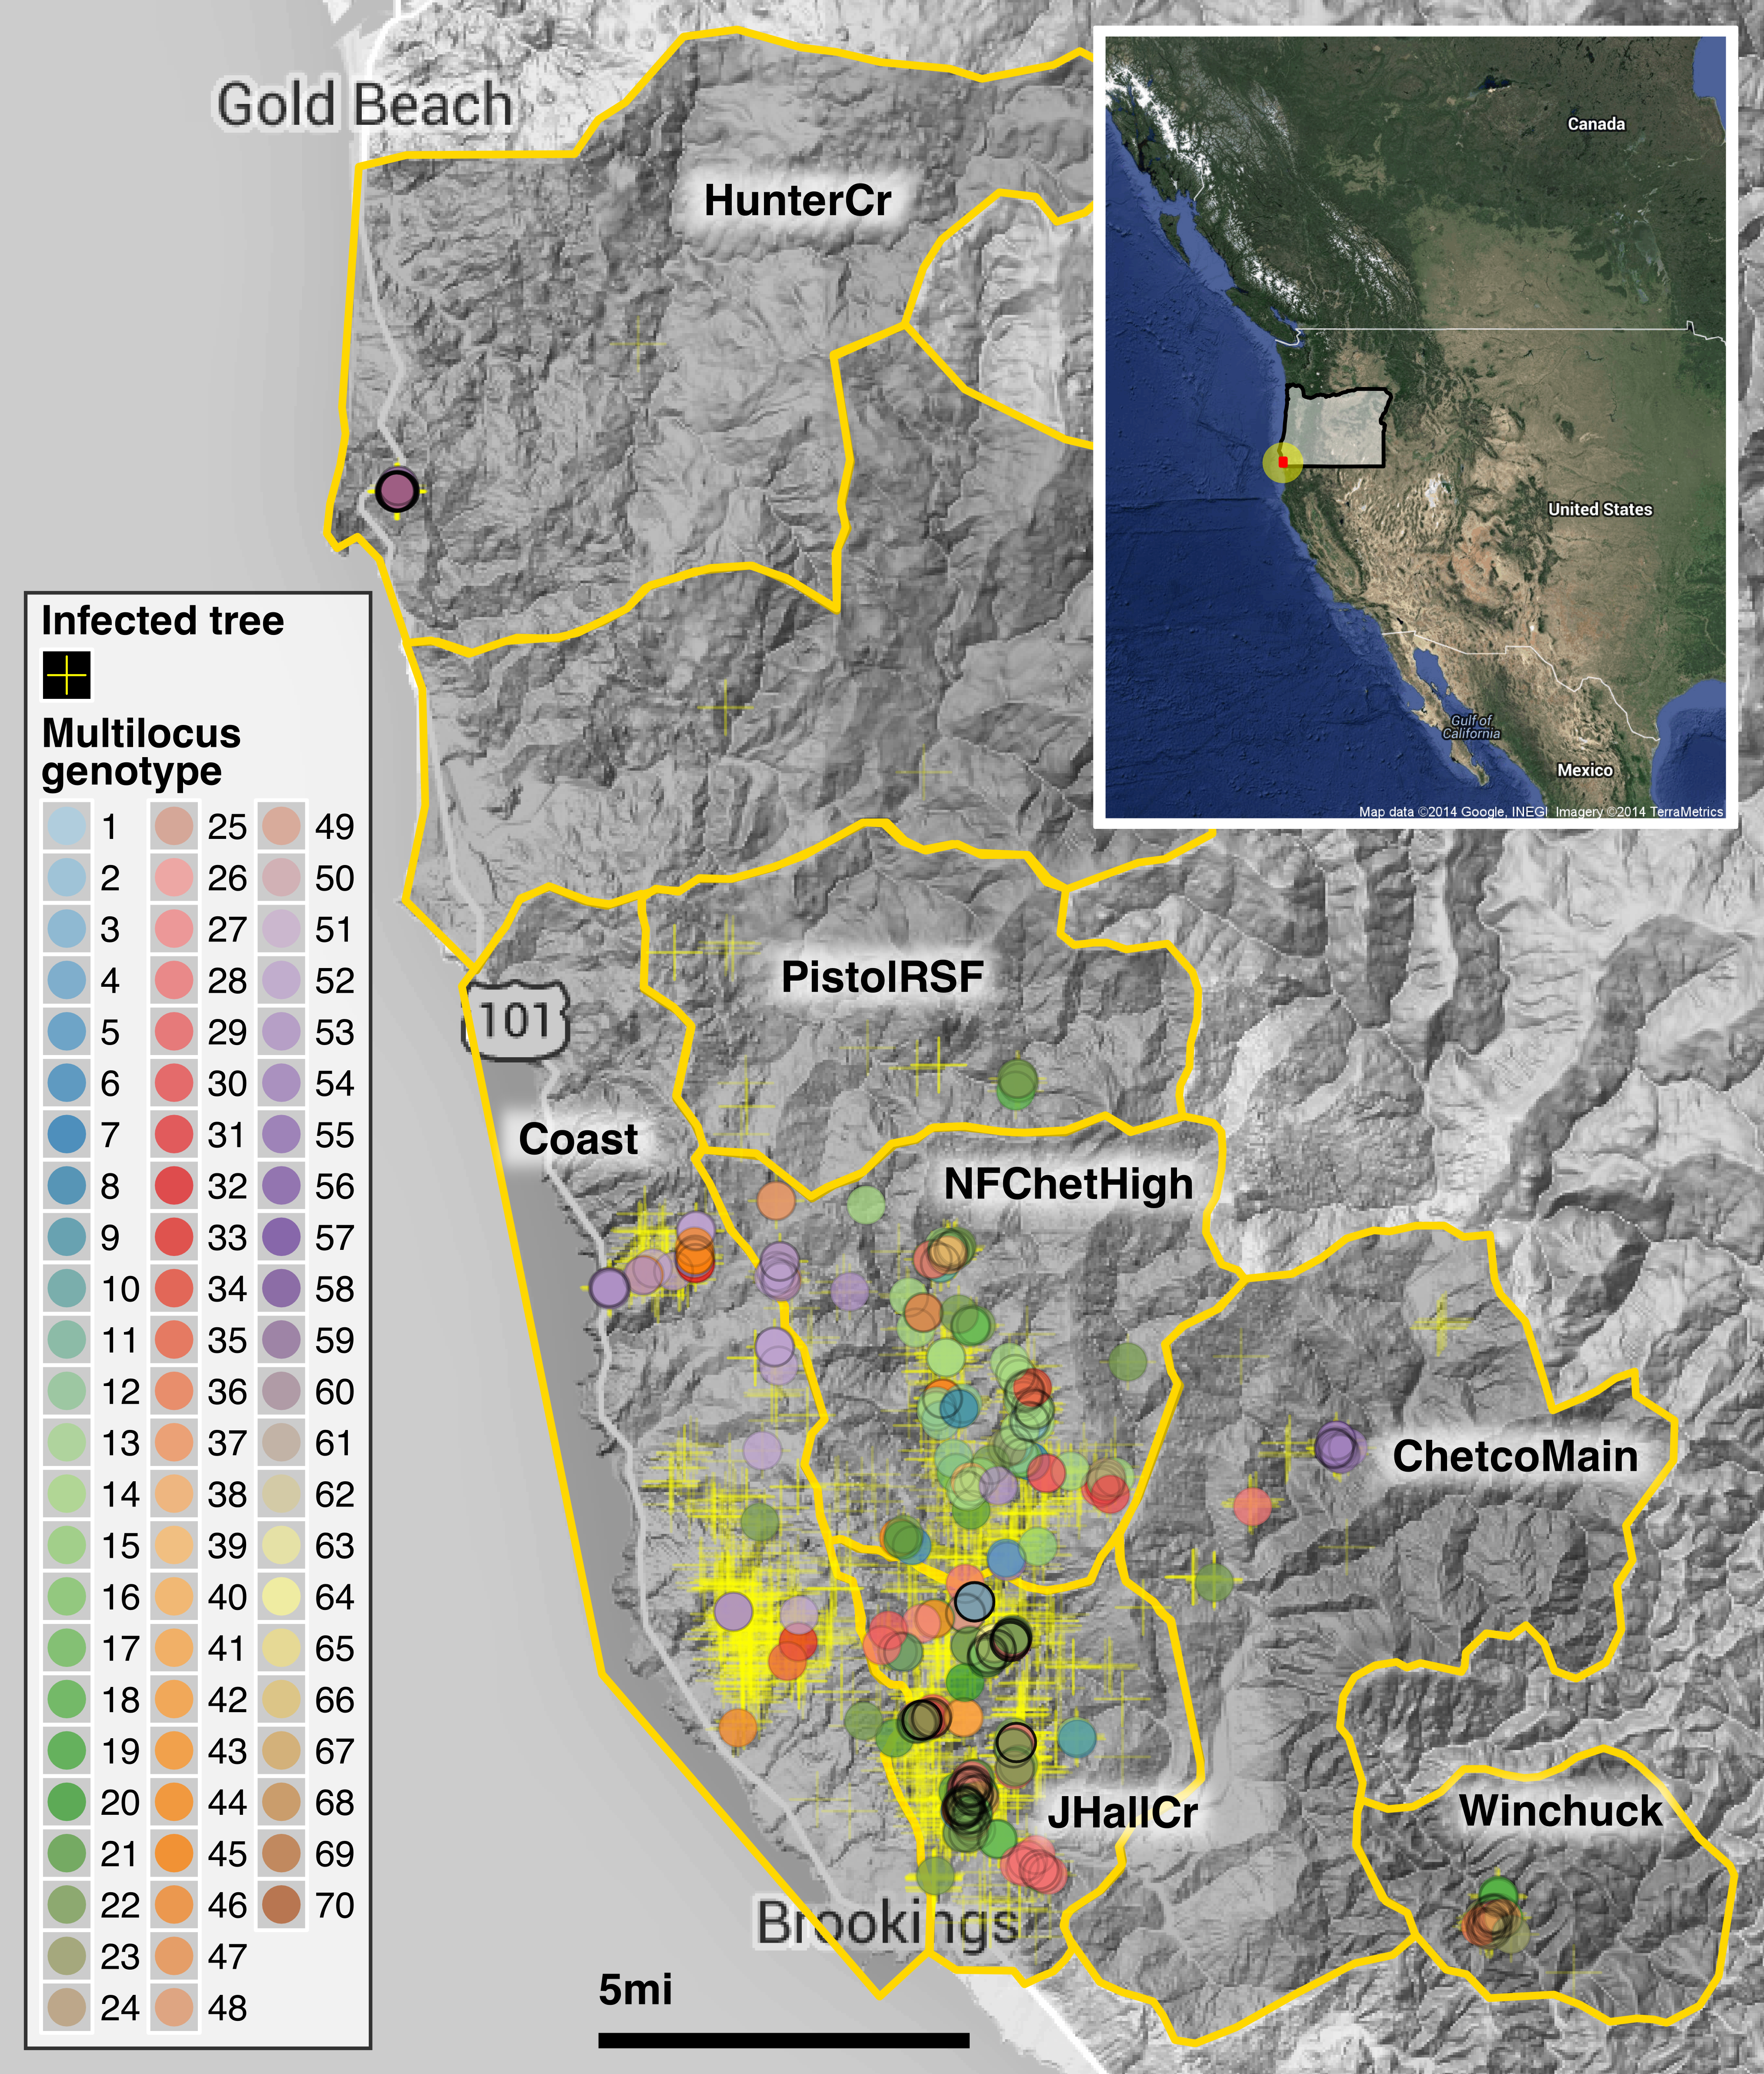
\includegraphics[width=0.8\linewidth]{figure/phytopathology/figure_1} 
  
  }
  
  \caption[Spatial distribution of the SOD epidemic and multilocus genotypes of
  \emph{Phytophthora ramorum} in Curry County, Oregon.]{Spatial distribution of the SOD epidemic and multilocus genotypes of
  \emph{Phytophthora ramorum} in Curry County, Oregon. The yellow crosses
  mark tanoak trees found positive for \emph{P. ramorum} during aerial
  surveys. A total of 70 multilocus genotypes have been identified between
  2001-2014 and are marked by color as shown in the legend. The
  abbreviations for regions shown in the map are explained in Table
  \ref{tab:ramorum1}. The inset shows the placement of Curry county (red
  dot) in SW Oregon.}\label{fig:ramorum1}
  \end{figure}
  
  \newpage
  
  \subsection{Sampling}\label{sampling}
  
  Commencing in 2001, 2-4 aerial surveys per year were conducted over the
  tanoak range by the Oregon Department of Forestry and the USDA Forest
  Service in Curry County. The survey detects recently killed tanoaks
  based on the reddish-brown color of foliage (Hansen et al.,
  \protect\hyperlink{ref-hansen2008epidemiology}{2008}). All trees
  identified by aerial surveys were ground checked and geographically
  referenced using a hand-held GPS instrument (Garmin GPS 12XL or 60CX,
  Garmin International, Olathe, KS). Bark or foliage samples were
  collected for determination of \emph{P. ramorum} presence by culturing
  in the field and laboratory. Host plants within the area of the
  delimitation survey, generally 300 feet, were also inspected and sampled
  if they were symptomatic. Maps of distribution were prepared using
  ArcView GIS version 3.3 and ArcMap version 10.2 (Environmental Systems
  Research Institute, Redlands, CA).
  
  \subsection{Isolation, identification and DNA
  extraction}\label{isolation-identification-and-dna-extraction}
  
  \begin{sidewaystable}[ph!]
  \caption{Summary of \emph{P. ramorum} isolates sampled in Oregon forests and multilocus genotypes (MLG)observed across regions and years.
  }
  \label{tab:ramorum1}
  \begin{tabular}{@{}lllrc@{}}
  \toprule
  \textbf{Abbreviation} & \textbf{Region name} & \textbf{Year} &
  \textbf{Number of} & \textbf{MLGs detected}\tabularnewline
   & & & \textbf{isolates} & \textbf{(region specific)}\tabularnewline
  \midrule
  JHallCr & Joe Hall Creek & 2001, 2002, 2003, 2004, & 244 & 30 (19)\tabularnewline
   &  & 2005, 2013, 2014 &  & \tabularnewline
  NFChetHigh & North Fork Chetco & 2003, 2012, 2013, 2014 & 114 & 35 (19)\tabularnewline
  Coast & Coastal Region & 2006, 2010, 2011, 2012, & 34 & 12 (7)\tabularnewline
   &  & 2013, 2014 &  & \tabularnewline
  HunterCr & Hunter Creek; Cape Sebastian & 2011 & 66 & 4 (4)\tabularnewline
  Winchuck &              ...             & 2012, 2013 & 35 & 9 (3)\tabularnewline
  ChetcoMain &              ...             & 2013, 2014 & 16 & 7 (1)\tabularnewline
  PistolRSF & Pistol River South Fork & 2013 & 4 & 2 (0)\tabularnewline
  \textbf{Total} & \textbf{-} & \textbf{2001-2014} & \textbf{513} &
  \textbf{70 (53)}\tabularnewline
  \bottomrule
  \end{tabular}
  \end{sidewaystable}
  
  Isolations were made from symptomatic plant tissue onto selective CARP
  agar (Difco corn meal agar, 10 ppm natamycin, 200pm NA-ampicillin, and
  10 ppm rifampicin) (Prospero et al.,
  \protect\hyperlink{ref-prospero2007population}{2007}). Candidate
  \emph{Phytophthora} cultures were transferred onto corn meal agar with
  30 ppm \(\beta\)-sitosterol. \emph{P. ramorum} identification was
  confirmed by microscopic inspection for presence of characteristic
  chlamydospores and deciduous sporangia (Werres et al.,
  \protect\hyperlink{ref-werres2001phytophthora}{2001}). Genomic DNA was
  extracted using either the FastDNA SPIN kit (MP Biomedicals, LLC;
  116540600) (Goss et al.,
  \protect\hyperlink{ref-goss2009population}{2009}) or the cetyltrimethyl
  ammonium bromide (CTAB )-chloroform-isopropanol method (Winton \&
  Hansen, \protect\hyperlink{ref-winton2001molecular}{2001}). Table
  \ref{tab:ramorum1} provides an overview of strains collected by year and
  region following regions as shown in figure \ref{fig:ramorum1}.
  
  \subsection{Genotyping, data validation, and
  harmonization}\label{genotyping-data-validation-and-harmonization}
  
  Five microsatellite loci were utilized in this analysis: PrMS6, Pr9C3,
  PrMS39, PrMS45, and PrMS43 (Grünwald et al.,
  \protect\hyperlink{ref-grunwald2009standardizing}{2009},
  \protect\hyperlink{ref-grunwald2008susceptibility}{2008}\protect\hyperlink{ref-grunwald2008susceptibility}{b};
  Prospero et al., \protect\hyperlink{ref-prospero2004isolation}{2004},
  \protect\hyperlink{ref-prospero2007population}{2007}). Genotyping (see
  specific protocols in supplementary text) of \emph{P. ramorum} strains
  collected 2001-2012 occurred over several years and in several
  laboratories, with different protocols and sequencers. Consequently, a
  concerted effort was made to create a comprehensive dataset with
  identical allele calls. To detect errors, allele calls from all five
  genotyped loci were generated for a subsample of 40 isolates
  representing the most common multilocus genotypes from the culture
  collection, and then compared to data from participating laboratories.
  Three of the five loci, PrMS6, Pr9C3, and PrMS39 had identical allele
  calls between laboratories for the subsampled isolates. The remaining
  two loci, PrMS45 and PrMS43, had allele calls that differed by a single
  bp between laboratories. Data from PrMS45 and PrMS43 were therefore
  corrected to allow consistent comparisons of allele calls. Given the
  varied nature of the genotyping data described above genotyping of
  \emph{P. ramorum} strains consists of two datasets including either 5
  loci (2001-14) or a newly developed, multiplexed method including 14
  loci (samples 2013-14) (Table \ref{tab:ramorum2}). Details on both
  genotyping methods can be found in the supplementary text \ref{text:S1}
  and figure \ref{fig:ramS1}.
  
  \begin{sidewaystable}[ph!]
  
  \caption[Newly multiplexed protocol for \emph{P. ramorum}
  primer sequences of simple sequence repeat (SSR) loci and final
  concentrations used to determine multilocus genotypes for four clonal
  lineages.]{(Caption on Next Page)}
  
  \label{tab:ramorum2}
  \begin{tabular}{@{}llllll@{}}
  \toprule
  \textbf{SSR Locus} & \textbf{Dye} & \textbf{Product} & \textbf{Primer sequence\textsuperscript{b}} &
  \textbf{Final conc.} & \textbf{Rxn}\tabularnewline
   &  & \textbf{(bp)\textsuperscript{c}} &  &
  \textbf{($\mu$M)} & \tabularnewline
  \midrule
  ILVOPrMS145abc\textsuperscript{f} & 6-FAM & 167-257 &
  \vtop{\hbox{\strut Fwd6FAM-TGGCAGTGTTCTTCAACAGC}\hbox{\strut Rev-\emph{GTTT}ATTCCCGTGAACAGCGTATC}}
  & 0.04 & 8-plex\tabularnewline
  PrMS39\textsuperscript{d} & NED & 130-258 &
  \vtop{\hbox{\strut FwdNED-GCACGGCCAGAGATTGATAG}\hbox{\strut Rev-\emph{GTTT}ATCTGCCGACGTGAAGAAGT}}
  & 0.07 & 8-plex\tabularnewline
  PrMS9C3\textsuperscript{d} & PET & 210-226 &
  \vtop{\hbox{\strut FwdVIC-TCACACGAAGCAGCAACTCT}\hbox{\strut Rev-\emph{GTTT}AGCGGCACTACGGAATACAT}}
  & 0.04 & 8-plex\tabularnewline
  ILVOPrMS79\textsuperscript{af} & 6-FAM & 342-396 &
  \vtop{\hbox{\strut Fwd6FAM-AGGCGGAAAACGTCAGAAC}\hbox{\strut Rev-\emph{GTTT}CTCGAGAGGCTGGAAGTACG}}
  & 0.15 & 8-plex\tabularnewline
  KI18\textsuperscript{e} & VIC & 217-279 &
  \vtop{\hbox{\strut FwdPET-TGCCATCACAACACAAATCC}\hbox{\strut Rev-\emph{GTT}TGTGCTATCTTTCCTGAACGG}}
  & 1.0 & 8-plex\tabularnewline
  KI64\textsuperscript{e} & NED & 342-401 &
  \vtop{\hbox{\strut FwdNED-GCGCTAAGAAAGACACTCCG}\hbox{\strut Rev-\emph{GTTT}CAACATGTAGCCATTGCAGG}}
  & 0.35 & 8-plex\tabularnewline
  PrMS45\textsuperscript{d} & VIC & 138-186 &
  \vtop{\hbox{\strut FwdVIC-CGTGCTGCATCTGGTGTAGT}\hbox{\strut Rev-GAAAGTCCGGATTTGCGTTA}}
  & 0.15 & 8-plex\tabularnewline
  PrMS6\textsuperscript{d} & PET & 165-168 &
  \vtop{\hbox{\strut FwdPET-AATCGATCTCTCGGCTTTGA}\hbox{\strut Rev-TATAGCCCCAGCTGCAACA}}
  & 0.15 & 8-plex\tabularnewline
  ILVOPrMS131\textsuperscript{f} & VIC & 146-414 &
  \vtop{\hbox{\strut FwdVIC-CGGCCGTTTTTGTAAGTTTG}\hbox{\strut Rev-\emph{GTTT}CAGATCAAACCAAAATCTGCTC}}
  & 0.2 & 2-plex\tabularnewline
  KI82ab\textsuperscript{e} & NED & 95-243 &
  \vtop{\hbox{\strut FwdNED-CCACGTCATTGGGTGACTTC}\hbox{\strut Rev-\emph{GTTT}CGTACAAGTCACGACTCCCC}}
  & 0.2 & 2-plex\tabularnewline
  PrMS43\textsuperscript{d} & 6-FAM & 122-493 &
  \vtop{\hbox{\strut Fwd6FAM-AAATATGCAAAAAGGCAGGA}\hbox{\strut Rev-\emph{GTTT}CCGCGTAACCTAGTCTGCTC}}
  & 0.3 & Simplex\tabularnewline
  \bottomrule
  \end{tabular}
  \end{sidewaystable}
  
  \newpage
  
  \renewcommand{\tablename}{Table Caption}
  \renewcommand{\thetable}{\arabic{chapter}.C\arabic{table}}
  
  \addtocounter{table}{-1}
  
  \vspace*{\fill}
  
  \begin{table}[ph!]
  \caption[Caption for Table \ref{tab:ramorum2}]{(Caption for Table 
  \ref{tab:ramorum2}) Newly multiplexed protocol for \emph{P. ramorum}
  primer sequences of simple sequence repeat (SSR) loci and final
  concentrations used to determine multilocus genotypes for four clonal
  lineages. PrMS6, Pr9C3, PrMS39, PrMS45, and PrMS43 were utilized in this
  study as they were commonly genotyped across all laboratories.
  \textsuperscript{a} ILVOPrMS79 amplifies three alleles in the NA1 lineage. The first two alleles are fixed and the third is polymorphic.
  \textsuperscript{b} Reverse (Rev) primer includes PIG tail addition except for PrMS45 and PrMS6. Indicated in italic.
  \textsuperscript{c} Product size range is for four lineages (EU1, EU2, NA1, NA2). Only the NA1 lineage has been reported in Curry County,OR forests.
  \textsuperscript{d} Described by Prospero et al. (\protect\hyperlink{ref-prospero2004isolation}{2004}) and/or Prospero et al. (\protect\hyperlink{ref-prospero2007population}{2007}).
  \textsuperscript{e} Described by Ivors et al. (\protect\hyperlink{ref-ivors2006microsatellite}{2006}).
  \textsuperscript{f} Described by Vercauteren et al. (\protect\hyperlink{ref-vercauteren2010clonal}{2010}), and Vercauteren et al.
  (\protect\hyperlink{ref-vercauteren2011identification}{2011}).}
  \label{cap:ramorum2}
  \end{table}\vspace*{\fill}
  
  \renewcommand{\tablename}{Table}
  \renewcommand{\thetable}{\arabic{chapter}.\arabic{table}}
  
  \newpage
  
  \subsection{Nursery populations}\label{nursery-populations}
  
  To determine if forest populations cluster with different nursery
  populations from Oregon or California, we used previously published data
  from our work to determine relationships among nursery and Curry County
  forest populations (Goss et al.,
  \protect\hyperlink{ref-goss2009population}{2009},
  \protect\hyperlink{ref-goss2011phytophthora}{2011}; Grünwald et al.,
  \protect\hyperlink{ref-grunwald2009standardizing}{2009}; Prospero et
  al., \protect\hyperlink{ref-prospero2009migration}{2009},
  \protect\hyperlink{ref-prospero2007population}{2007}).
  
  \subsection{Data analysis}\label{data-analysis-1}
  
  All individuals genotyped for this effort belonged to the NA1 clonal
  lineage (Grünwald et al.,
  \protect\hyperlink{ref-grunwald2009standardizing}{2009}). Thus, all
  analyses presented here focused on describing the clonal dynamic using
  model-free approaches that avoid violation of population genetic theory.
  Samples were grouped into different multilocus genotypes (MLGs) defined
  by the unique combination of alleles across all observed loci from the
  consensus five SSR loci genotyped across all years. For identification
  purposes, unique MLGs were then assigned an arbitrary number from 1 to
  the total number of observed MLGs. Population genetic analysis was
  conducted using the computer and statistical language R (R Core Team,
  \protect\hyperlink{ref-R2014}{2014}) using various packages as well as R
  functions written specifically for this project (see github link below).
  Graphs and figures were created using the R packages \emph{ggplot2, ape,
  igraph, ggmap,} and \emph{poppr} (Csardi \& Nepusz,
  \protect\hyperlink{ref-csardi2006igraph}{2006}; Kahle \& Wickham,
  \protect\hyperlink{ref-khale2013ggmap}{2013}; Kamvar et al.,
  \protect\hyperlink{ref-kamvar2014poppr}{2014}\protect\hyperlink{ref-kamvar2014poppr}{b};
  Paradis et al., \protect\hyperlink{ref-paradis2004ape}{2004}; Wickham,
  \protect\hyperlink{ref-wickham2009ggplot2}{2009}). Within-locus allelic
  diversity was analyzed across and within years and regions using the
  function \texttt{locus\_table()} from the R package \emph{poppr} (Table
  \ref{tab:ramtabS1}) (Kamvar et al.,
  \protect\hyperlink{ref-kamvar2014poppr}{2014}\protect\hyperlink{ref-kamvar2014poppr}{b}).
  To address the temporal and spatial aspects of the data, populations
  were analyzed both by year isolated and watershed region (Table
  \ref{tab:ramorum1}; Fig. \ref{fig:ramorum1}). Watershed regions were
  drawn with ArcMap version 10.2 (Environmental Systems Research
  Institute, Redlands, CA). The regions represent drainages or portions of
  drainages in which infected trees were discovered as the disease
  progressed over time. In most cases, ridgelines dividing drainages
  formed the boundary of a region. These regions were saved as shapefiles
  and imported into R with \emph{rgdal} (Bivand et al.,
  \protect\hyperlink{ref-bivand2014rgdal}{2014}).
  
  Genotypic diversity was analyzed within and across years and
  populations, with the Shannon-Wiener index (\emph{H}) and the Stoddard
  and Taylor's index (\emph{G}), (Shannon,
  \protect\hyperlink{ref-shannon2001mathematical}{1948}; Stoddart \&
  Taylor, \protect\hyperlink{ref-stoddart1988genotypic}{1988}). Both
  \emph{G} and \emph{H} measure genotypic diversity, combining richness
  and evenness. If all genotypes are equally abundant, then the value of
  \emph{G} will be the number of MLGs and the value of \emph{H} will be
  the natural log of the number of MLGs. Both \emph{G} and \emph{H} are
  used as they weigh more or less abundant MLGs more heavily, respectively
  (Grünwald et al., \protect\hyperlink{ref-grunwald2003analysis}{2003}).
  Evenness was calculated as \emph{E\textsubscript{5}}, which is an
  estimator of evenness that utilizes both \emph{H} and \emph{G} that
  gives a ratio of the number of abundant genotypes to rare genotypes
  (Grünwald et al., \protect\hyperlink{ref-grunwald2003analysis}{2003};
  Ludwig \& Reynolds, \protect\hyperlink{ref-ludwig1988statistical}{1988};
  Pielou, \protect\hyperlink{ref-pielou1975ecological}{1975}). These were
  calculated with the R packages \emph{poppr} and \emph{vegan} (Kamvar et
  al.,
  \protect\hyperlink{ref-kamvar2014poppr}{2014}\protect\hyperlink{ref-kamvar2014poppr}{b};
  Oksanen et al., \protect\hyperlink{ref-oksanen2013vegan}{2013}).
  Confidence intervals were calculated using the R package \emph{boot}
  with 9,999 bootstrap resamplings (Canty \& Ripley,
  \protect\hyperlink{ref-canty2015boot}{2015}). Richness, or the expected
  number of MLGs (\emph{eMLG}), was calculated using rarefaction from the
  R packages \emph{poppr} and \emph{vegan} (Heck et al.,
  \protect\hyperlink{ref-heck1975explicit}{1975}; Hurlbert,
  \protect\hyperlink{ref-hurlbert1971nonconcept}{1971}). Some statistics
  (AMOVA, genotypic diversity, index of association, allelic diversity,
  and Nei's distance) were also performed on clone-censored data where
  each MLG was represented once per population hierarchy.
  
  Because the analysis of genotypic diversity, richness and evenness is
  agnostic to specific alleles within MLGs, assessment of genetic
  relatedness between MLGs was performed using the function
  \texttt{bruvo.dist()} using \emph{poppr}, which calculates Bruvo's
  genetic distance, utilizing a stepwise mutation model for microsatellite
  loci (Bruvo et al., \protect\hyperlink{ref-bruvo2004simple}{2004};
  Kamvar et al.,
  \protect\hyperlink{ref-kamvar2014poppr}{2014}\protect\hyperlink{ref-kamvar2014poppr}{b}).
  This distance thus gives a more fine-scale picture of relationships
  between individuals than band-sharing models. These relationships were
  visualized with minimum spanning networks generated using the R packages
  \emph{igraph} and \emph{poppr} (Csardi \& Nepusz,
  \protect\hyperlink{ref-csardi2006igraph}{2006}; Kamvar et al.,
  \protect\hyperlink{ref-kamvar2014poppr}{2014}\protect\hyperlink{ref-kamvar2014poppr}{b}).
  
  If the epidemic had a single origin, a correlation between genetic and
  geographic distance would be expected as populations acquire mutations
  over time and clonally diverge regardless of rates of spread. This was
  tested by performing Mantel tests across all hierarchical levels in the
  data set utilizing the function \texttt{mantel.randtest()} in the R
  package \emph{ade4} between Bruvo's distance as described above and
  Euclidean distances between geographic coordinates (Dray \& Dufour,
  \protect\hyperlink{ref-dray2007ade4}{2007}; Mantel,
  \protect\hyperlink{ref-mantel1967detection}{1967}). \emph{P}-values were
  calculated using 99,999 bootstrap replicates.
  
  As the eradication efforts destroy the immediate habitat in an infected
  area, one question that we wanted to address was whether or not
  genotypes were clustering to specific regions or if they were evenly
  spread throughout Curry County (Prospero et al.,
  \protect\hyperlink{ref-prospero2007population}{2007}). This was tested
  using three methods: bootstrap analysis of Nei's genetic distance,
  Analysis of MOlecular VAriance (AMOVA), and Discriminant Analysis of
  Principal Components (DAPC) in the R packages \emph{poppr}, \emph{ade4},
  and \emph{adegenet} (Excoffier et al.,
  \protect\hyperlink{ref-excoffier1992analysis}{1992}; Jombart et al.,
  \protect\hyperlink{ref-jombart2010discriminant}{2010}; Kamvar et al.,
  \protect\hyperlink{ref-kamvar2014poppr}{2014}\protect\hyperlink{ref-kamvar2014poppr}{b}).
  The bootstrap analysis utilized 10,000 bootstrap replicates treating
  loci as independent units with the function \texttt{aboot()} in
  \emph{poppr} and was visualized as an unrooted neighbor-joining tree in
  figtree v. 1.4.2 (Figure \ref{fig:ramorum5}). AMOVA utilizes a distance
  matrix between genotypes for which hierarchical partitions are defined
  and attempts to analyze the variation within samples, between samples,
  between subpopulations within populations and finally between
  populations. In this case, we used both the hierarchies of samples
  within years within regions and samples within regions within years.
  DAPC is a multivariate, model-free approach to clustering based on prior
  population information (Jombart et al.,
  \protect\hyperlink{ref-jombart2010discriminant}{2010}). This allows us
  to analyze the population structure by assessing how well samples can be
  reassigned into previously defined populations. Both DAPC and AMOVA were
  run with and without Hunter Creek and Pistol River South Fork due to
  isolated genotypes and small sample size, respectively. For the DAPC
  analysis, these removed populations had their origins predicted from the
  DAPC object using the function predict.dapc in the R package
  \emph{adegenet} (Jombart et al.,
  \protect\hyperlink{ref-jombart2010discriminant}{2010}).
  
  Since DAPC is sensitive to the number of principal components used in
  analysis, the function \texttt{xvalDapc()} from the R package
  \emph{adegenet} was used to select the correct number of principal
  components with 1,000 replicates using a training set of 90\% of the
  data. The number of principal components was chosen based on the
  criteria that it had to produce the highest average percent of
  successful reassignment and lowest root mean squared error (Jombart et
  al., \protect\hyperlink{ref-jombart2010discriminant}{2010}). Significant
  deviations from random population structure was tested in AMOVA
  utilizing the function \texttt{randtest()} from the R package
  \emph{ade4} with 9,999 bootstrap replicates (Dray \& Dufour,
  \protect\hyperlink{ref-dray2007ade4}{2007}).
  
  All data and R scripts to reproduce the analyses shown here are
  deposited publicly on github
  (\url{https://github.com/grunwaldlab/Sudden_Oak_Death_in_Oregon_Forests})
  and citable (DOI: 10.5281/zenodo.13007).
  
  \section{Results}\label{results}
  
  \subsection{Demographic pattern and genetic
  diversity}\label{demographic-pattern-and-genetic-diversity}
  
  The epidemic has expanded over time from the initial focus in Joe Hall
  Creek NE of Brookings, Oregon mostly north (first to N Fork Chetco High)
  and northwest (Coast, Pistol River South Fork), but also east (Chetco
  Main and Winchuck) (Fig. \ref{fig:ramorum1}; Table \ref{tab:ramorum1}).
  To date a total of 70 multilocus genotypes have been found in forest
  populations (Table \ref{tab:ramorum1}). MLG 22 is most abundant and the
  only MLG detected across the whole period (although it was not sampled
  in every year) (Fig. \ref{fig:ramorum2}). MLG 59, the second most
  abundant MLG, was only detected in 2011 and has a high frequency due to
  the sampling design applied: all 2011 strains were sampled in one
  concentrated area in the northwestern sampling range geographically
  distant from any other location (Fig. \ref{fig:ramorum2}). Given that
  sampling strategies for some years were not comprehensive, samples from
  some years have to be interpreted with caution (e.g., 2005-6, 2010-11).
  Samples from 2013 and 2014 are sampled from all regions and can be
  considered more representative.
  
  \begin{figure}
  
  {\centering \includegraphics[width=0.4\linewidth]{figure/phytopathology/figure_2} 
  
  }
  
  \caption[Rank distribution of multilocus genotypes (MLGs) of \emph{P. ramorum}
  and recovery per year.]{Rank distribution of multilocus genotypes (MLGs) of \emph{P. ramorum}
  and recovery per year. The vertical axis denotes unique MLGs detected in
  the whole data set with decreasing abundance as indicated by the barplot
  on the right side. The horizontal axis indicates year of sampling. Each
  numbered circle represents the number of observations of each MLG with
  lines connecting genotypes found in multiple years.}\label{fig:ramorum2}
  \end{figure}
  
  \newpage
  
  Allelic and genotype diversity within loci revealed that PrMS43 had, on
  average, the highest number of alleles (n = 18). All other loci had 5 or
  fewer alleles with a moderate to high amount of diversity (Table
  \ref{tab:ramtabS2}). Nevertheless, the genotype accumulation curve
  showed a slight plateau, indicating that we have enough power in our
  data to describe a significant number of MLGs (Fig. \ref{fig:ramS2}).
  Genotypic diversity (\emph{H} = 2.98, \emph{G} = 8.64), evenness
  (\emph{E\textsubscript{5}} = 0.41), and richness (\emph{eMLG} = 7) were
  low as expected for a clonal population slowly accumulating mutations
  over space and time (Table \ref{tab:ramtabS3}). A pattern of increasing
  diversity across years (with number of MLGs not fewer than 10) was also
  observed (Table \ref{tab:ramtabS3}). The minimum spanning network showed
  that MLGs 17, 22, and 28 clustered in the center of the network and had
  the highest number of connections to other genotypes in the forest
  populations (Fig. \ref{fig:ramorum3}). Most genotypes were connected to
  their immediate neighbors by a genetic distance of 0.05 or the
  equivalent of one mutational step across 5 diploid loci.
  
  \begin{figure}
  
  {\centering \includegraphics[width=0.75\linewidth]{figure/phytopathology/figure_3} 
  
  }
  
  \caption[Minimum spanning network based on Bruvo's genetic distance for
  microsatellite markers for \emph{P. ramorum} populations.]{Minimum spanning network based on Bruvo's genetic distance for
  microsatellite markers for \emph{P. ramorum} populations. Nodes
  (circles) represent individual multilocus genotypes. The 10 most
  abundant forest genotypes are labeled with their MLG designation. Node
  colors represent population membership proportional to the pie size.
  Node sizes are relatively scaled to \emph{log\textsubscript{1.75}n,}
  where \emph{n} is the number of samples in the nodes to avoid node
  overlap. Edges (lines) represent minimum genetic distance between
  individuals determined by Prim's algorithm. Nodes that are more closely
  related will have darker and thicker edges whereas nodes more distantly
  related will have lighter and thinner edges or no edge at all.
  Reticulation was introduced by finding exact ties in genetic distance
  after Prim's algorithm was run. Subgroups of \textgreater{}3 MLGs where
  all nodes are no more than one mutational step (d = 0.05) away from its
  neighbors, are highlighted in arbitrary colors.}\label{fig:ramorum3}
  \end{figure}
  
  \newpage
  
  \subsection{Spatial Correlation}\label{spatial-correlation}
  
  A Mantel test revealed significant correlations of genetic distance and
  geographic distance for most samples collected after 2003 (Table
  \ref{tab:ramorum3}). When partitioned by year, this correlation appears
  to increase and become more pronounced with the progression of the
  epidemic. When partitioned by region, those that are closer to the
  origin of the epidemic (Joe Hall Creek and N Fork Chetco River) show
  significant correlation. When the overall mantel test was run without
  Hunter Creek, the correlation coefficient was reduced (0.175), but was
  still significant (\emph{p} = 0.0001).
  
  \begin{sidewaystable}[ph!]
  \centering
  \caption[Table of correlation coefficients generated across
  forest regions and years of \emph{P. ramorum} isolates using the Mantel
  test.]{Table of correlation coefficients generated across
  forest regions and years of \emph{P. ramorum} isolates using the Mantel
  test. Euclidean distances were calculated from geographic coordinates
  while genetic distance was based on Bruvo's distance. Significance of
  values are based on 99,999 Monte-Carlo permutations and marked as
  follows: \^{} $\leq$ 0.05, \~{} $\leq$ 0.01, * $\leq$ 0.001, - = no data, NaN =
  insufficient data for analysis.}
  \label{tab:ramorum3}
  \begin{tabular}{@{}lllllllllllll@{}}
  \toprule
  & \textbf{2001} & \textbf{2002} & \textbf{2003} & \textbf{2004} &
  \textbf{2005} & \textbf{2006} & \textbf{2010} & \textbf{2011} &
  \textbf{2012} & \textbf{2013} & \textbf{2014} &
  \textbf{Pooled}\tabularnewline
  \midrule
  JHallCr & 0.06 & 0.24 & 0.14* & 0.28* & NaN & - & - & - & - & 0.18\~{}
  & NaN & 0.14*\tabularnewline
  NFChetHigh & - & - & NaN & - & - & - & - & - & 0.68 & 0.41* & -0.23 &
  0.35*\tabularnewline
  Coast & - & - & - & - & - & NaN & NaN & NaN & NaN & 0.55\^{} & -0.25 &
  0.13\tabularnewline
  HunterCr & - & - & - & - & - & - & - & 0.06 & - & - & - &
  0.06\tabularnewline
  Winchuck & - & - & - & - & - & - & - & - & 0.41\~{} & 0.03 & - &
  0.11\tabularnewline
  ChetcoMain & - & - & - & - & - & - & - & - & - & 0.53 & NaN &
  0.63*\tabularnewline
  PistolRSF & - & - & - & - & - & - & - & - & - & 0.94 & - &
  0.94\tabularnewline
  Pooled & 0.06 & 0.24 & 0.13* & 0.28* & NaN & NaN & NaN & 0.87* &
  0.59* & 0.15* & 0.14\^{} & \textbf{0.52*}\tabularnewline
  \bottomrule
  \end{tabular}
  \end{sidewaystable}
  
  \subsection{Population
  differentiation}\label{population-differentiation}
  
  Cluster analysis of populations with respect to year using Nei's genetic
  distance showed no significant (\textgreater{}70\%) bootstrap support
  for any clades, but does show that these tend to cluster by region as
  opposed to year (Fig. \ref{fig:ramS3}). AMOVA analysis revealed
  significant population structure between regions on both clone-corrected
  (with respect to hierarchy) and uncorrected data sets (Table
  \ref{tab:ramtab4}). Significant structure was only found between years
  within regions on the uncorrected data set. Both patterns were observed
  without Hunter Creek and Pistol River South Fork isolates. DAPC
  clustering showed that the first discriminant component separated Hunter
  Creek from all other regions and the second discriminant component shows
  a gradient from Joe Hall Creek to the coast (Fig. \ref{fig:ramfig4}).
  This distinction was reflected in the percent of correct posterior
  assignment of isolates to their original populations. Over the whole
  data set there was an 81.5\% assignment- success rate. Hunter Creek
  received 100\% successful reassignment. Joe Hall Creek, Winchuck, and
  Coast all had \textgreater{}85\% successful reassignment whereas Chetco
  Main, North Fork of the Chetco, and Pistol River South Fork all had
  \textless{}69\% successful reassignment (Fig. \ref{fig:ramS4}). The
  isolation of the Hunter Creek isolates in the DAPC analysis was found to
  be mainly driven by allele 493 at locus PrMS43 (Fig. \ref{fig:ramS5}).
  The only other population to share this allele was Joe Hall Creek where
  it was present in a total of 4 isolates, and only isolates found in the
  coastal region or North Fork Chetco contained the allele 489, which is
  one mutational step away in a stepwise mutation model of a
  tetranucleotide repeat locus. When DAPC was run without Hunter Creek and
  Pistol River South Fork data, percent successful reassignment for all
  regions did not change significantly. Prediction of sources for the
  Hunter Creek data revealed that over 98\% of the genotypes were assigned
  to the Coast with a 99\% probability.
  
  \begin{sidewaystable}[ph!]
  \centering
  \caption[AMOVA table generated comparing \textit{P. ramorum} isolates for
  two different hierarchies]{AMOVA table generated comparing \emph{P. ramorum} isolates for two
  different hierarchies, year within region and region within year,
  respectively. Results are rounded to three significant figures. Clone
  corrected results are provided in parentheses. P values are based on
  9,999 permutations.} 
  \label{tab:ramtab4}
  \begin{tabular}{lccccc}
   \textbf{Heirarchy} & \textbf{df} & \textbf{Sum of squares} & \textbf{Variation (\%)} & \textbf{\textit{P}} & \textbf{$\phi$ statistic} \\ 
    \midrule
  \textbf{Region by year} &  &  &  &  &  \\ 
    Between region & 10 (10) & 160 (21) & 11.6 (3) & 0.366 (0.175) & 0.448 (0.101) \\ 
    Between year within region & 12 (12) & 59.5 (19.1) & 33.3 (7.07) & 1e-04 (2e-04) & 0.376 (0.0729) \\ 
    Within year within region & 490 (129) & 281 (141) & 55.2 (89.9) & 1e-04 (1e-04) & 0.116 (0.03) \\ 
    \textbf{Year by region} &  &  &  &  &  \\ 
    Between year & 6 (6) & 197 (23) & 45 (12.3) & 1e-04 (1e-04) & 0.496 (0.12) \\ 
    Between region within year & 16 (16) & 22.5 (17.2) & 4.56 (-0.283) & 1e-04 (0.446) & 0.0829 (-0.00323) \\ 
    Within region within year & 490 (129) & 281 (141) & 50.4 (88) & 1e-04 (1e-04) & 0.45 (0.123) \\ 
     \bottomrule
  \end{tabular}
  \end{sidewaystable}
  
  \begin{figure}
  
  {\centering \includegraphics[width=0.8\linewidth]{dissertation_files/figure-latex/ramfig4-1} 
  
  }
  
  \caption[Scatterplot from DAPC of the first two principal components
  discriminating \emph{P. ramorum} populations by regions.]{Scatterplot from DAPC of the first two principal components
  discriminating \emph{P. ramorum} populations by regions. Points
  represent individual observations. Colors and lines represent population
  membership. Inertia ellipses represent an analog of a 67\% confidence
  interval based on a bivariate normal distribution.}\label{fig:ramfig4}
  \end{figure}
  
  \newpage
  
  \subsection{Clustering of forest with nursery
  populations}\label{clustering-of-forest-with-nursery-populations}
  
  We used previously published data to determine if nursery populations in
  California or Oregon could have been source populations for the Oregon
  forest epidemic (Goss et al.,
  \protect\hyperlink{ref-goss2009population}{2009},
  \protect\hyperlink{ref-goss2011phytophthora}{2011}; Grünwald et al.,
  \protect\hyperlink{ref-grunwald2009standardizing}{2009}; Prospero et
  al., \protect\hyperlink{ref-prospero2009migration}{2009},
  \protect\hyperlink{ref-prospero2007population}{2007}). Nursery data
  included 40 MLGs across 216 samples of NA1 clones. Of these 40, 12 MLGs
  matched the forest sample and 28 MLGs were unique to the nurseries. The
  only region that did not contain genotypes that matched those found in
  nurseries was Pistol River South Fork. When considering those 12
  genotypes that were present in both data sets, with the exception of Joe
  Hall Creek, all genotypes were first isolated from nurseries before
  discovery in the forest. At the most variable locus, PrMS43, both
  nursery populations had the allele 281 at frequencies of 4.5\% and 4.9\%
  for CA and OR, respectively. This allele was not observed in the forest
  population. Both populations contained allele 489 at \textgreater{}10\%
  frequency and the CA nursery population contained allele 493 at a
  frequency of 1.4\%.
  
  When nursery genotypes were added to the minimum spanning network, MLGs
  found at Hunter Creek, previously isolated in the network, connected by
  only a single MLG from the coast, gained more connections to nursery
  MLGs. Clustering with Nei's distance revealed the Nursery isolates from
  CA consistently clustering closest with Hunter Creek isolates in both
  clone-corrected and uncorrected data sets (Fig. \ref{fig:ramorum5}).
  DAPC clustering revealed a decrease in overall assignment-success rate
  at 78\%. The nursery isolates received 74\% and 83\% assignment success
  for CA and OR nurseries, respectively.
  
  \begin{figure}
  
  {\centering \includegraphics[width=0.8\linewidth]{figure/phytopathology/figure_5} 
  
  }
  
  \caption[Unrooted, neighbor-joining tree with 10,000 bootstrap replicates of
  Nei's genetic distance for \emph{P. ramorum} populations defined by
  region.]{Unrooted, neighbor-joining tree with 10,000 bootstrap replicates of
  Nei's genetic distance for \emph{P. ramorum} populations defined by
  region. Tip labels are colored by region. Branches with bootstrap values
  greater than 50\% are shown in blue. Nursery populations are shown as
  originating from California (CA) or Oregon (OR).}\label{fig:ramorum5}
  \end{figure}
  
  \newpage
  
  The assignment successes for the regions before or after inclusion of
  nursery data changed less than 5\% for all regions except for the coast,
  which saw a decrease of 17.6\% when nursery populations were included
  (Fig. \ref{fig:ramS4}). Prediction of sources for nursery genotypes
  against the forest data revealed that 48\% of these nursery isolates
  were predicted to share membership with the coast at \(\geq\) 95\%
  probability (Fig. \ref{fig:ramS6}, \ref{fig:ramS7}). A total of 3.2\% of
  the isolates were predicted to share membership with Hunter Creek at
  \(\geq\) 99.9\% membership probability. Furthermore, 21.75\% of the
  nursery data could not be assigned to any of the forest populations at
  \textgreater{}60\% probability.
  
  Since 3.2\% of the nursery isolates had a very strong signal for Hunter
  Creek, we predicted sources for Hunter Creek isolates when considering
  nursery isolates. This approach determines if Hunter Creek isolates
  cluster more readily with nursery or coast populations. Indeed, 92\% of
  the Hunter Creek isolates were predicted to share membership with
  California nurseries at \(\geq\) 99\% membership probability (Fig.
  \ref{fig:ramS8}). No Hunter Creek isolate was predicted to share
  membership with a forest population at \textgreater{}0.45\% membership
  probability.
  
  \section{Discussion}\label{discussion-1}
  
  To date populations monitored from 2001-14 show presence of only the NA1
  clonal lineage observed previously (Prospero et al.,
  \protect\hyperlink{ref-prospero2009migration}{2009},
  \protect\hyperlink{ref-prospero2007population}{2007}). The fact that
  individuals belonging to the EU1 and NA2 clonal lineages have not been
  found in Oregon forests, despite their presence on the west coast from
  British Columbia to California is welcome news (Goss et al.,
  \protect\hyperlink{ref-goss2009population}{2009},
  \protect\hyperlink{ref-goss2011phytophthora}{2011}; Grünwald et al.,
  \protect\hyperlink{ref-grunwald2012emergence}{2012}). The lack of EU1 or
  NA2 isolates provides evidence that monitoring for \emph{P. ramorum} in
  nurseries by federal and state agencies is helping avoid emergence of
  new clones in Oregon's Forests.
  
  Our analysis provides support for a most parsimonious scenario of two
  introductions into Curry county from nurseries: one initial introduction
  into Curry County sometime before detection of the first infected
  tanoaks in 2001 from California (or less likely Oregon) nurseries
  followed by a second introduction into the Hunter Creek area again from
  nurseries. The relative position of the nursery populations in the
  minimum spanning network and DAPC scatter plot (Fig. \ref{fig:ramorum3},
  \ref{fig:ramfig4}) suggest that the introductions from nurseries were
  rare, though more even sampling and migration models could disprove this
  hypothesis. Since 2001, the epidemic has spread clonally throughout
  Southwestern Curry County mostly north, but also west, towards the
  coast, and southeast. This clonal spread of the pathogen from the Joe
  Hall area is supported partially by Mantel tests showing significant
  levels of isolation by distance in years following 2002 (Table
  \ref{tab:ramorum3}) along with significant AMOVA results across regions
  (Table \ref{tab:ramtab4}). The populations sampled in 2011 in Hunter
  Creek (Cape Sebastian) appear to have originated from a new source and
  cluster into a distinct group based on DAPC (Fig. \ref{fig:ramfig4}).
  Based on the minimum spanning network, this population would appear
  isolated in the epidemic if it were not for MLG 32, which is connected
  with MLG 33 (found on the coast in 2010) by one mutational step at locus
  PrMS43. This, in turn, is connected with the other MLGs from Hunter
  Creek by one mutational step at locus PrMS39. When considering
  clustering via Bruvo's distance in combination with data from nursery
  populations, however, these genotypes from Hunter Creek appear to be
  more similar to California nursery populations (Fig. \ref{fig:ramorum3})
  than Oregon forest populations. Predictions based on DAPC place samples
  from Hunter Creek as coming from California nurseries (Fig.
  \ref{fig:ramS8}). This, in combination with the observation that purely
  forest genotypes (i.e.~those only found in the forest) are connected to
  Hunter Creek genotypes through nursery genotypes, indicates a possible
  contribution from nursery populations to the epidemic. This is supported
  by the observation that all population level clustering, with and
  without clone correction, places the Hunter Creek isolates adjacent to
  the nursery isolates from CA (Fig. \ref{fig:ramfig4},
  \ref{fig:ramorum5}). This appears to be driven by the high frequency of
  allele 246 at locus PrMS39, which interestingly appears to segregate in
  an east to west fashion and is increasing in frequency over time (Fig.
  \ref{fig:ramS9}, \ref{fig:ramS10}). This, along with the results from
  the DAPC clustering and subsequent prediction (Fig. \ref{fig:ramS6},
  \ref{fig:ramS7}) provide weak support for a potential third introduction
  into the coastal region from nurseries sometime after the Hunter Creek
  introduction event.
  
  An interesting aspect is the observation that there appeared to be more
  than one cluster of genotypes introduced into the Joe Hall area during
  the early stages of the epidemic. The two dominant clusters that
  appeared were the ones that contained MLG 22 and MLG 68. The former has
  been found in the most recent sampling year, whereas the latter has not
  been observed since 2005 or beyond the Joe Hall area. This latter group
  was also the most distantly related group overall, more distant than
  some nursery genotypes. While it is clear that the eradication effort
  has not been entirely successful, there is some evidence that it is
  having an effect as a major genotype cluster has effectively been
  eradicated, although disappearance of MLGs could also be explained by
  being less fit than lineages dominating now.
  
  The Curry County epidemic is in many ways different from the epidemic in
  California. When introduced into California in the mid 1990's, the
  causal agent of sudden oak death was unknown and thus gave it time to
  clonally expand and diversify as management strategies in natural forest
  systems were limited (Rizzo et al.,
  \protect\hyperlink{ref-rizzo2002phytophthora}{2002}). With the foresight
  of the epidemic in central California, the ODF was able to implement a
  quarantine effort against the import of hosts as soon as the causal
  agent was known (A Kanaskie, pers. comm.). This quarantine along with
  aggressive eradication efforts have affected the spread of \emph{P.
  ramorum} (Mascheretti et al.,
  \protect\hyperlink{ref-mascheretti2008reconstruction}{2008}). Drawing
  conclusions from previous population studies in California and applying
  them to the Oregon epidemic should be undertaken with great care given
  the drastically differing management scenarios (Mascheretti et al.,
  \protect\hyperlink{ref-mascheretti2009genetic}{2009},
  \protect\hyperlink{ref-mascheretti2008reconstruction}{2008}).
  
  Our work has some inherent drawbacks. Given the cost of aerial surveys
  and subsequent ground crew work, and the fact that trees are eradicated
  once found, populations are not hierarchically sampled across all years.
  The destructive nature of the management approach means that it was not
  possible to conduct controlled ecological experiments focusing on
  effects of climate and rainfall on the spread of disease as was possible
  in California trials (Eyre et al.,
  \protect\hyperlink{ref-eyre2013poulation}{2013}). In addition, most of
  our work only used 5 microsatellite loci for genotyping. Ideally, more
  loci should have been used as was done in other studies (Croucher et
  al., \protect\hyperlink{ref-croucher2013combining}{2013}). Although only
  5 loci were used, clear patterns of population dynamics in space and
  time emerged and the MLG accumulation curve supported the fact that loci
  are informative. Finally, the populations genotyped here are clonal and
  belong to the NA1 clonal lineage. Thus, much of the analytical power
  provided by population genetic theory does not apply given that basic
  assumptions would be violated (Grünwald \& Goss,
  \protect\hyperlink{ref-grunwald2011evolution}{2011}). Our work uses
  appropriate methods to infer patterns that are model free, yet
  informative such as spatial clustering. Thus, we believe that this work
  provides novel and important insights into the \emph{P. ramorum}
  population biology in the Siskiyou forest. Our data indicates that there
  might have been at least two introductions into Oregon forests from
  nurseries. The nature of the data does not allow inference of
  directional migrations given the uneven sampling strategy and moderate
  number of loci used across all years. We are currently exploring
  genotyping-by-sequencing (GBS) as a method that could provide further
  detail on how these populations evolved over space and time (Elshire et
  al., \protect\hyperlink{ref-elshire2011robust}{2011}). GBS can provide
  richer detail by providing codominant SNP data across several thousand
  loci sampling the whole genome.
  
  \section{Acknowledgements}\label{acknowledgements-2}
  
  This work was supported in part by US Department of Agriculture (USDA)
  Agricultural Research Service Grant 5358-22000-039-00D, USDA APHIS, the
  USDA-ARS Floriculture Nursery Initiative, the Oregon Department of
  Agriculture/Oregon Association of Nurseries (ODA-OAN) and the
  USDA-Forest Service Forest Health Monitoring Program.
  
  \section{Supplementary Material}\label{supplementary-material}
  
  \subsection{Supplementary Text}\label{text:S1}
  
  For the years up to and including 2012, the multilocus genotype (MLG) of
  each \emph{P. ramorum} strain was determined based on microsatellite
  analysis of five loci, PrMS6, Pr9C3, PrMS39, PrMS45 and PrMS43, using
  previously published protocols (Grünwald et al.,
  \protect\hyperlink{ref-grunwald2009standardizing}{2009},
  \protect\hyperlink{ref-grunwald2008susceptibility}{2008}\protect\hyperlink{ref-grunwald2008susceptibility}{b};
  Prospero et al., \protect\hyperlink{ref-prospero2004isolation}{2004},
  \protect\hyperlink{ref-prospero2007population}{2007}). Multilocus
  genotyping of \emph{P. ramorum} strains collected in 2013 and 2014
  included an extra nine loci, KI18, KI64, KI82a, KI82b, ILVOPrMS79,
  ILVOPrMS131, ILVOPrMS145a, ILVOPrMS145b, ILVOPrMS145c which are
  amplified by an additional six primer pairs (Ivors et al.,
  \protect\hyperlink{ref-ivors2006microsatellite}{2006}; Vercauteren et
  al., \protect\hyperlink{ref-vercauteren2010clonal}{2010},
  \protect\hyperlink{ref-vercauteren2011identification}{2011}). The locus
  ILVOPrMS79, amplifies up to three alleles, however two separate loci
  have yet to be described (Vercauteren et al.,
  \protect\hyperlink{ref-vercauteren2011identification}{2011}). The
  addition of nine loci to the genotyping assay coincided with the
  discovery by the Oregon Department of Agriculture of an EU1 \emph{P.
  ramorum} isolate in a Curry County nursery in 2012. Preceding 2012, only
  NA1 isolates had been found in Curry County. Because different loci are
  polymorphic for different clonal lineages, the entire panel of 14 loci
  was necessary to adequately describe the \emph{P. ramorum} population in
  the event that multiple lineages were discovered in the forest.
  
  Methods for genotyping the 2013 and 2014 \emph{P. ramorum} strains with
  all 14 loci use new multiplex protocol. Previously published primers
  were modified by the addition of a 5' PIG tail ``GTTT'' to reverse
  primers in an effort to reduced stutter peaks and hence to better
  facilitate allele scoring (Table \ref{tab:ramorum2}) (Brownstein et al.,
  \protect\hyperlink{ref-brownstein1996modulation}{1996}). In two cases
  (PrMS45, PrMS6), a PIG tail was not added to reverse primers to simplify
  scoring of overlapping alleles. Also, where a T residue was already
  present at the 5' end of a reverse primer, as in the case of KI18, a
  ``GTT'' was added instead of ``GTTT''. Forward primers were assigned
  fluorescent labels, 6-FAM, NED, VIC, or PET, to facilitate separation of
  overlapping markers (Table \ref{tab:ramorum2}). Primer concentrations
  were determined by visual inspection of electropherograms (Table
  \ref{tab:ramorum2}).
  
  Amplification of all 14 loci was separated into three reactions (8-plex,
  2-plex and simplex). The simplex reaction amplified the PrMS43 locus
  using methods described earlier (Grünwald et al.,
  \protect\hyperlink{ref-grunwald2009standardizing}{2009}; Prospero et
  al., \protect\hyperlink{ref-prospero2007population}{2007}). The 8-plex
  and 2-plex amplified the remaining loci and were performed under
  identical conditions with the exception of primers and primer
  concentrations (Table \ref{tab:ramorum2}). For the multiplex reactions,
  the QIAGEN Type-it Mutation Detect PCR Kit (QIAGEN, 206343, Valencia,
  CA) was used. Multiplex PCR reactions were performed in 5\(\mu\)l
  volumes with 10ng template DNA and1X final buffer concentration.
  Amplifications were run on a Veriti thermal cycler (Life Technologies,
  Grand Island, NY) with an initial denaturation at 95 \(^{\circ}\)C for 5
  min, followed by 33 cycles of 95 \(^{\circ}\)C for 30 s, 60
  \(^{\circ}\)C for 90 s, and 72 \(^{\circ}\)C for 20 s, and a final
  extension at 60 \(^{\circ}\)C for 30 min. Genotyping prior to 2012
  included three reference DNA lineages (EU1, NA1, and NA2). After 2012, a
  fourth lineage (EU2) was added as a reference (Poucke et al.,
  \protect\hyperlink{ref-vanpoucke2012discovery}{2012}).
  
  Electrophoresis and visualization of all microsatellites were performed
  on ABI3100, ABI3100 Avant, or ABI3130 genetic analyzers (Applied
  Biosystems). For evaluation of the loci, genotyped prior to 2013, the
  PCR products were diluted 10 times in ultrapure H\textsubscript{2}0 and
  1.5 \(\mu\)l of diluted product was added to both 8.5 \(\mu\)l of
  Hi-Di\textsuperscript{TM} Formamide (Applied Biosystems, 4311320) and
  0.25 \(\mu\)l of GeneScan\textsuperscript{TM} 500
  LIZ\textsuperscript{TM} size standard (Applied Biosystems, 4322682). The
  simplex reaction (PrMS43) was also diluted 10 times while the 8-plex and
  2-plex products were diluted 75 times. After dilution, 2.5 \(\mu\)l of
  the 8-plex, 2-plex and simplex products were added to 7.5 \(\mu\)l of
  Hi-Di\textsuperscript{TM} Formamide containing
  GeneScan\textsuperscript{TM} 500 LIZ\textsuperscript{TM} size standard
  at a ratio of 6 \(\mu\)l size standard to 1 ml Hi-Di\textsuperscript{TM}
  Formamide. Allele sizing was determined using
  GeneMapper\textregistered{} v3.7 and v5.0 software (Applied Biosystems).
  
  \setcounter{figure}{0} \setcounter{table}{0}
  \renewcommand{\figurename}{Supplementary Figure}
  \renewcommand{\tablename}{Supplementary Table}
  \renewcommand{\thefigure}{\arabic{chapter}.S\arabic{figure}}
  \renewcommand{\thetable}{\arabic{chapter}.S\arabic{table}}
  
  \subsection{Supplementary Figures}\label{supplementary-figures}
  
  \begin{figure}
  
  {\centering \includegraphics[width=1\linewidth]{figure/phytopathology/figureS1} 
  
  }
  
  \caption[Diagram of DNA extraction, genotyping, and sequencing protocols 
  utilized by two labs from 2001 to 2014.]{Diagram of DNA extraction, genotyping, and sequencing protocols 
  utilized by two labs from 2001 to 2014. See supplementary text for details.}\label{fig:ramS1}
  \end{figure}
  
  \begin{figure}
  
  {\centering \includegraphics[width=0.8\linewidth]{dissertation_files/figure-latex/ramS2-1} 
  
  }
  
  \caption[Genotype accumulation curve for OR forest \emph{P. ramorum} isolates.]{Genotype accumulation curve for OR forest \emph{P. ramorum} isolates.
  The vertical axis denotes the number of observed MLGs, from 0 to the
  observed number of MLG in the forest populations, for a number of loci,
  indicated on the horizontal axis, randomly sampled without replacement.
  Each boxplot contains 1,000 random samples representing different
  possible combinations of \emph{n} loci. The horizontal red dashed line
  represents 90\% of MLG resolution.}\label{fig:ramS2}
  \end{figure}
  
  \begin{figure}
  
  {\centering \includegraphics[width=0.8\linewidth]{figure/phytopathology/figureS3} 
  
  }
  
  \caption[Neighbor joining tree based on Nei's distance of the forest \emph{P.
  ramorum} isolates by region with respect to year.]{Neighbor joining tree based on Nei's distance of the forest \emph{P.
  ramorum} isolates by region with respect to year. Bootstrap values
  \textgreater{} 50\% of 10,000 replicates are shown in blue.}\label{fig:ramS3}
  \end{figure}
  
  \begin{figure}
  
  {\centering \includegraphics[width=0.8\linewidth]{dissertation_files/figure-latex/ramS4-1} 
  
  }
  
  \caption[Loading plot from DAPC of \emph{P. ramorum from} forest populations
  showing the contribution of alleles to the first DAPC eigenvalue
  separating Hunter Creek isolates from all other regions.]{Loading plot from DAPC of \emph{P. ramorum from} forest populations
  showing the contribution of alleles to the first DAPC eigenvalue
  separating Hunter Creek isolates from all other regions.}\label{fig:ramS4}
  \end{figure}
  
  \begin{figure}
  
  {\centering \includegraphics[width=0.8\linewidth]{figure/phytopathology/figureS5} 
  
  }
  
  \caption[Fractions of posterior population assignments from DAPC clustering of
  \emph{P. ramorum} isolates from forest populations.]{Fractions of posterior population assignments from DAPC clustering of
  \emph{P. ramorum} isolates from forest populations. The horizontal axis
  represents the fraction of samples whose posterior group membership
  matched their prior group membership on the vertical axis. Shape
  indicates presence or absence of nursery populations in the DAPC.}\label{fig:ramS5}
  \end{figure}
  
  \begin{figure}
  
  {\centering \includegraphics[width=0.8\linewidth]{figure/phytopathology/figureS6} 
  
  }
  
  \caption[Prediction of nursery genotypes of \emph{P. ramorum} into forest
  watershed regions.]{Prediction of nursery genotypes of \emph{P. ramorum} into forest
  watershed regions. The horizontal axis indicates the fraction of nursery
  genotypes to be predicted to be similar to the populations on the
  vertical axis with a 95, 99, and 99.9\% probability as indicated by the
  size of the points.}\label{fig:ramS6}
  \end{figure}
  
  \begin{figure}
  
  {\centering \includegraphics[width=0.8\linewidth]{figure/phytopathology/figureS7} 
  
  }
  
  \caption[Graphical representation of prediction of nursery isolates of \emph{P.
  ramorum} into forest watershed regions.]{Graphical representation of prediction of nursery isolates of \emph{P.
  ramorum} into forest watershed regions. Each column represents a
  different isolate. Colors within the columns represent membership
  probabilities from forest populations.}\label{fig:ramS7}
  \end{figure}
  
  \begin{figure}
  
  {\centering \includegraphics[width=0.8\linewidth]{figure/phytopathology/figureS8} 
  
  }
  
  \caption[Graphical representation of predicted membership of \emph{P. ramorum}
  isolates from Hunter Creek and Pistol River South Fork in forest and
  nursery populations.]{Graphical representation of predicted membership of \emph{P. ramorum}
  isolates from Hunter Creek and Pistol River South Fork in forest and
  nursery populations. Each column represents a different isolate. Colors
  within the columns represent membership probabilities from the
  populations indicated in the legend.}\label{fig:ramS8}
  \end{figure}
  
  \begin{figure}
  
  {\centering \includegraphics[width=0.8\linewidth]{figure/phytopathology/figureS9} 
  
  }
  
  \caption[Allele frequencies of locus PrMS39 of \emph{P. ramorum} across years of
  the forest populations.]{Allele frequencies of locus PrMS39 of \emph{P. ramorum} across years of
  the forest populations. Years 2005 through 2011 have been omitted due to
  small sample sizes and outlier genotypes.}\label{fig:ramS9}
  \end{figure}
  
  \begin{figure}
  
  {\centering \includegraphics[width=0.8\linewidth]{figure/phytopathology/figureS10} 
  
  }
  
  \caption[Map of the infected area in Curry county showing the \emph{P. ramorum}
  genotypes at locus PrMS39.]{Map of the infected area in Curry county showing the \emph{P. ramorum}
  genotypes at locus PrMS39. Each colored circle represents a different
  forest isolate while each yellow cross represents a sampled tree. Yellow
  borders denote different regions.}\label{fig:ramS10}
  \end{figure}
  
  \subsection{Supplementary Tables}\label{supplementary-tables}
  
  \begin{longtable}[c]{@{}lrrrrr@{}}
  
  \caption[Mean allelic diversity metrics of
  clone-corrected populations of \emph{Phytophthora ramorum} sampled in
  Curry County, Oregon between 2001-14 causing sudden oak death.]{(Caption on next page)}\tabularnewline
  \label{tab:ramtabS1}
  
  \textbf{Population} & \textbf{MLG} & \textbf{alleles} & \textbf{1-D} & \textbf{Hexp} & \textbf{Evenness}\tabularnewline
  \midrule
  \endfirsthead
  \multicolumn{6}{c}%
  {{\tablename\ \thetable{} -- continued from previous page}} \\
  \textbf{Population} & \textbf{MLG} & \textbf{alleles} & \textbf{1-D} & \textbf{Hexp} & \textbf{Evenness}\tabularnewline
  \midrule
  \endhead
  
  \multicolumn{6}{r}{\textbf{Continued on next page...}} \\
  \endfoot
  
  \endlastfoot
  
  ChetcoMain & 7 & 3.0 & 0.58 & 0.97 & 0.94\tabularnewline
  Coast & 12 & 3.8 & 0.59 & 0.97 & 0.96\tabularnewline
  HunterCr & 4 & 2.6 & 0.56 & 0.96 & 0.95\tabularnewline
  JHallCr & 30 & 4.4 & 0.57 & 0.91 & 0.89\tabularnewline
  NFChetHigh & 35 & 4.8 & 0.60 & 0.90 & 0.89\tabularnewline
  PistolRSF & 2 & 2.4 & 0.55 & 1.00 & 1.00\tabularnewline
  Winchuck & 9 & 3.4 & 0.56 & 0.94 & 0.92\tabularnewline
  2001 & 10 & 3.6 & 0.56 & 0.94 & 0.91\tabularnewline
  2002 & 9 & 3.0 & 0.56 & 0.94 & 0.93\tabularnewline
  2003 & 20 & 4.2 & 0.56 & 0.90 & 0.89\tabularnewline
  2004 & 8 & 2.8 & 0.50 & 0.84 & 0.85\tabularnewline
  2005 & 2 & 2.4 & 0.50 & 0.90 & 0.92\tabularnewline
  2006 & 1 & 2.0 & 0.50 & 1.00 & 1.00\tabularnewline
  2010 & 1 & 2.0 & 0.50 & 1.00 & 1.00\tabularnewline
  2011 & 6 & 3.0 & 0.58 & 0.98 & 0.96\tabularnewline
  2012 & 7 & 3.2 & 0.58 & 0.96 & 0.95\tabularnewline
  2013 & 47 & 5.4 & 0.60 & 0.89 & 0.90\tabularnewline
  2014 & 17 & 3.8 & 0.59 & 0.97 & 0.93\tabularnewline
  pooled & 70 & 6.0 & 0.60 & 0.89 & 0.90\tabularnewline
  \bottomrule
  \end{longtable}
  
  \newpage
  
  \renewcommand{\tablename}{Supplementary Table Caption}
  \renewcommand{\thetable}{\arabic{chapter}.C\arabic{table}}
  
  \addtocounter{table}{-1}
  
  \vspace*{\fill}
  
  \begin{table}[ph!]
  \caption[Caption for Table \ref{tab:ramtabS1}]{(Caption for Table 
  \ref{tab:ramtabS1}) Mean allelic diversity metrics of
  clone-corrected populations of \emph{Phytophthora ramorum} sampled in
  Curry County, Oregon between 2001-14 causing sudden oak death. MLG =
  Number of Multilocus Genotypes; alleles = Average number of alleles
  across 5 loci; 1-D = Simpson's Index averaged across 5 loci; Hexp =
  Nei's 1978 expected heterozygosity; Evenness = Evenness averaged across
  5 loci}
  \label{cap:ramcapS1}
  \end{table}\vspace*{\fill}
  
  \renewcommand{\tablename}{Supplementary Table}
  \renewcommand{\thetable}{\arabic{chapter}.S\arabic{table}}
  
  
  \newpage
  
  \begin{longtable}[]{@{}lrrrr@{}}
  \caption{\label{tab:ramtabS2} Allelic diversity metrics for each locus of
  clone-corrected \emph{Phytophthora ramorum} data in Curry County, Oregon
  between 2001-14 causing sudden oak death. alleles = number of observed
  alleles; 1-D = Simpson's Index; Hexp = Nei's 1978 expected
  heterozygosity; E.5 = Evenness}\tabularnewline
  \toprule
  locus & alleles & 1-D & Hexp & E.5\tabularnewline
  \midrule
  \endfirsthead
  \toprule
  locus & alleles & 1-D & Hexp & E.5\tabularnewline
  \midrule
  \endhead
  PrMS6 & 2 & 0.50 & 0.99 & 0.99\tabularnewline
  Pr9C3 & 2 & 0.50 & 0.99 & 0.99\tabularnewline
  PrMS39 & 5 & 0.62 & 0.78 & 0.78\tabularnewline
  PrMS45 & 3 & 0.51 & 0.76 & 0.95\tabularnewline
  PrMS43 & 18 & 0.89 & 0.95 & 0.78\tabularnewline
  mean & 6 & 0.60 & 0.89 & 0.90\tabularnewline
  \bottomrule
  \end{longtable}
  
  \begin{sidewaystable}[ph!]
  \centering
  \caption[Genotypic diversity metrics or populations of
  textit{Phytophthora ramorum} sampled in Curry County, Oregon between 2001-14
  causing sudden oak death.
  ]{(Caption on Next Page)} 
  \label{tab:ramtabS3}
  \begin{tabular}{lrrrrlllrr}
    \toprule
  Population & N & MLG & eMLG & SE & H & G & E.5 & rbarD & p.rD \\ 
    \midrule
  2001 &  39 &  10 & 3.65 & 1.16 & 1.19 (0.61-1.48) & 1.9 (1.38-2.81) & 0.4 (0.4-0.57) & -0.07 & 1.00 \\ 
    2002 &  36 &   9 & 4.20 & 1.13 & 1.37 (0.79-1.64) & 2.34 (1.52-3.52) & 0.45 (0.43-0.65) & 0.19 & 0.00 \\ 
    2003 & 102 &  20 & 4.75 & 1.30 & 1.81 (1.39-2) & 2.92 (2.19-3.96) & 0.38 (0.36-0.49) & 0.14 & 0.00 \\ 
    2004 &  35 &   8 & 4.56 & 1.01 & 1.57 (1.12-1.76) & 3.53 (2.3-4.77) & 0.66 (0.56-0.84) & 0.18 & 0.00 \\ 
    2005 &   2 &   2 & 2.00 & 0.00 & 0.69 (0-0.69) & 2 (1-2) & 1 (1-1) &  &  \\ 
    2006 &   1 &   1 & 1.00 & 0.00 & 0 (0-0) & 1 (1-1) & NaN (NA) &  &  \\ 
    2010 &   1 &   1 & 1.00 & 0.00 & 0 (0-0) & 1 (1-1) & NaN (NA) &  &  \\ 
    2011 &  68 &   6 & 2.15 & 0.83 & 0.56 (0.26-0.79) & 1.32 (1.13-1.59) & 0.42 (0.38-0.56) & 0.18 & 0.00 \\ 
    2012 &  20 &   7 & 5.01 & 0.92 & 1.62 (1.03-1.78) & 4 (2.2-5.26) & 0.74 (0.59-0.92) & -0.17 & 1.00 \\ 
    2013 & 179 &  47 & 7.74 & 1.20 & 3.15 (2.83-3.17) & 13.8 (10.2-16.3) & 0.57 (0.54-0.7) & 0.03 & 0.00 \\ 
    2014 &  30 &  17 & 8.09 & 1.03 & 2.67 (2.08-2.61) & 12.2 (6.16-12.2) & 0.83 (0.69-0.93) & -0.01 & 0.56 \\ 
    JHallCr & 244 &  30 & 4.89 & 1.33 & 1.97 (1.69-2.12) & 3.13 (2.57-3.83) & 0.34 (0.33-0.41) & 0.10 & 0.00 \\ 
    NFChetHigh & 114 &  35 & 6.81 & 1.34 & 2.74 (2.3-2.82) & 7.07 (4.8-9.88) & 0.42 (0.4-0.59) & 0.07 & 0.00 \\ 
    Coast &  34 &  12 & 5.91 & 1.17 & 2.05 (1.49-2.16) & 5.56 (3.36-7.22) & 0.68 (0.61-0.85) & 0.28 & 0.00 \\ 
    HunterCr &  66 &   4 & 1.88 & 0.69 & 0.42 (0.18-0.62) & 1.24 (1.1-1.46) & 0.46 (0.39-0.6) & -0.05 & 1.00 \\ 
    Winchuck &  35 &   9 & 4.29 & 1.07 & 1.47 (0.95-1.7) & 2.88 (1.89-4.15) & 0.56 (0.49-0.77) & -0.01 & 0.76 \\ 
    ChetcoMain &  16 &   7 & 5.00 & 0.93 & 1.45 (0.69-1.69) & 2.84 (1.49-4.74) & 0.56 (0.49-0.88) & 0.40 & 0.00 \\ 
    PistolRSF &   4 &   2 & 2.00 & 0.00 & 0.56 (0-0.69) & 1.6 (1-2) & 0.8 (0.8-1) &  &  \\ 
    Total & 513 &  70 & 6.95 & 1.33 & 2.98 (2.78-3.04) & 8.64 (7.19-10.1) & 0.41 (0.39-0.48) & 0.08 & 0.00 \\ 
     \bottomrule
  \end{tabular}
  \end{sidewaystable}
  
  \newpage
  
  \renewcommand{\tablename}{Supplementary Table Caption}
  \renewcommand{\thetable}{\arabic{chapter}.C\arabic{table}}
  
  \addtocounter{table}{-1}
  
  \vspace*{\fill}
  
  \begin{table}[ph!]
  \caption[Caption for Table \ref{tab:ramtabS3}]{(Caption for Table 
  \ref{tab:ramtabS3}) Genotypic diversity metrics or populations of
  \textit{Phytophthora ramorum} sampled in Curry County, Oregon between 2001-14
  causing sudden oak death. Pop = Population name (Total == Pooled)
  N = Census population size
  MLG = Number of unique multilocus genotypes (MLG) observed
  eMLG = Number of expected MLG based on rarefaction at smallest N >= 10
  SE = Standard error of rarefaction analysis
  H = Shannon-Wiener Index of MLG diversity (95\% CI in parentheses)
  G = Stoddart and Taylor's Index of MLG diversity (95\% CI in parentheses)
  E.5 = Evenness (95\% CI in parentheses)
  rbarD = Standardized index of association
  p.rbarD = p-value for the standardized index of association based on 999 permutations
  NaN = Insufficient data for analysis}
  \label{cap:ramcapS3}
  \end{table}\vspace*{\fill}
  
  \renewcommand{\tablename}{Supplementary Table}
  \renewcommand{\thetable}{\arabic{chapter}.S\arabic{table}}
  
  
  \newpage
  
  \renewcommand{\figurename}{Figure}
  \renewcommand{\tablename}{Table}
  \renewcommand{\thefigure}{\arabic{chapter}.\arabic{figure}}
  \renewcommand{\thetable}{\arabic{chapter}.\arabic{table}}
  
  \chapter{Factors Influencing Inference of Clonality in Diploid
  Populations}\label{factors-influencing-inference-of-clonality-in-diploid-populations}
  
  \singlespacing
  
  \begin{center}
  
  
  Zhian N. Kamvar and Niklaus J. Grünwald
  
  
  
  \end{center}\vspace*{\fill}
  
  Target Journal: \textbf{Molecular Ecology}
  
  \doublespacing
  \newpage
  
  \section{Abstract}\label{abstract-3}
  
  The index of association is a measure of multilocus linkage
  disequilibrium, which reflects the deviation of observed genetic
  variation from expected. In sexual populations, loci are randomly
  assorting due to recombination, resulting in a near-zero value of the
  index of association. In clonal populations, recombination is
  non-existent, meaning that loci are passed from parent to offspring in a
  non-independent fashion, resulting in a significantly non-zero value of
  the index of association. We build on previous work by investigating the
  effect of sample size, mutation rate, and clone correction on the power
  of the index of association to detect clonal reproduction in simulated
  data sets generated with microsatellite and genomic markers. Our
  findings suggest that power decreases with small sample sizes and low
  allelic diversity, and physical linkage in genomic markers does not
  affect power if permutation tests are performed with linkage groups. We
  hope that these novel insights provide useful to the study of molecular
  pathogens.
  
  \section{Introduction}\label{introduction-4}
  
  Population genetic theory is largely based on model populations such as
  the neutral Wright-Fisher model in which populations are assumed to be
  infinitely large, with discrete generations, randomly assorting alleles,
  with no migration and no mutation (Hartl \& Clark,
  \protect\hyperlink{ref-hartl1997principles}{2007}; Nielsen \& Slatkin,
  \protect\hyperlink{ref-nielsen2013introduction}{2013}). By using such
  reductionist models, population geneticists are able to reduce the
  complexity and enable analyses to ask fundamental questions and test
  hypotheses about evolutionary processes that could explain population
  structure and history.
  
  These neutral models, however, cannot be applied to populations whose
  life history violate the fundamental assumption of random assortment of
  alleles, such as populations that undergo clonal reproduction (Milgroom,
  \protect\hyperlink{ref-milgroom1996recombination}{1996}; Orive,
  \protect\hyperlink{ref-orive1993effective}{1993}). For many clonal
  populations, the contribution of genetic variation from mutation is
  greater than that of recombination. While this increases the risk of the
  accumulation of deleterious mutations, the two-fold cost of sex is
  drastically reduced, meaning that selectively advantageous combinations
  of alleles are maintained (Heitman et al.,
  \protect\hyperlink{ref-heitman2012evolution}{2012}).
  
  Pathogenic microorganisms can reproduce sexually or clonally (Milgroom,
  \protect\hyperlink{ref-milgroom1996recombination}{1996}; Tibayrenc,
  \protect\hyperlink{ref-tibayrenc1996towards}{1996}). Diseases caused by
  these organisms are in part managed by the use of antimicrobial
  compounds that kill these organisms. Detecting recombination in
  populations of pathogenic microorganisms is therefore important for the
  implementation of rational management strategies as a prevalence of
  sexual reproduction could lead to the repeated emergence of novel,
  resistant genotypes (de Meeûs et al.,
  \protect\hyperlink{ref-de2006molecular}{2006}; Goss et al.,
  \protect\hyperlink{ref-goss2014irish}{2014}; Milgroom,
  \protect\hyperlink{ref-milgroom1996recombination}{1996}; Nieuwenhuis \&
  James, \protect\hyperlink{ref-nieuwenhuis2016frequency}{2016}; Smith et
  al., \protect\hyperlink{ref-smith1993how}{1993}).
  
  Several studies have attempted to infer the degree of sex in populations
  that undergo clonal reproduction (Ali et al.,
  \protect\hyperlink{ref-ali2016cloncase}{2016}; Balloux et al.,
  \protect\hyperlink{ref-balloux2003population}{2003}; de Meeûs \&
  Balloux, \protect\hyperlink{ref-de2004clonal}{2004}; Nieuwenhuis \&
  James, \protect\hyperlink{ref-nieuwenhuis2016frequency}{2016}; Smith et
  al., \protect\hyperlink{ref-smith1993how}{1993}). For populations with
  well-defined sexual and clonal phases occurring at separate times, such
  as rust fungi, methods like \emph{CloNcaSe} are effective for estimating
  the rate of sexual reproduction and effective population size (Ali et
  al., \protect\hyperlink{ref-ali2016cloncase}{2016}). However, this
  method cannot be applied to populations where the reproductive cycle is
  not partitioned into discrete generations.
  
  Simply detecting the presence of clonal reproduction, however can be
  useful in and of itself (Milgroom,
  \protect\hyperlink{ref-milgroom1996recombination}{1996}). A method
  commonly used to assess this is the index of association (\(I_A\)), and
  its standardized version, \(\bar{r}_d\), which measure multilocus
  linkage disequilibrium (Agapow \& Burt,
  \protect\hyperlink{ref-Agapow_2001}{2001}; Brown et al.,
  \protect\hyperlink{ref-brown1980multilocus}{1980}; de Meeûs \& Balloux,
  \protect\hyperlink{ref-de2004clonal}{2004}; Haubold et al.,
  \protect\hyperlink{ref-haubold1998detecting}{1998}; Kamvar et al.,
  \protect\hyperlink{ref-kamvar2014poppr}{2014}\protect\hyperlink{ref-kamvar2014poppr}{b};
  Smith et al., \protect\hyperlink{ref-smith1993how}{1993}). The value of
  \(I_A\), as shown in equation \eqref{eq:ia}, is measured as the ratio of
  observed variance (\(V_O\)) and expected variance (\(V_E\)) in genetic
  distance between samples (Agapow \& Burt,
  \protect\hyperlink{ref-Agapow_2001}{2001}; Smith et al.,
  \protect\hyperlink{ref-smith1993how}{1993}):
  
  \begin{equation}
  I_A = \frac{V_O}{V_E} - 1 \label{eq:ia}
  \end{equation}
  
  The expected variance is practically modeled as the sum of the variances
  over \emph{m} loci: \(V_E = \sum^m{var_j}\) (Agapow \& Burt,
  \protect\hyperlink{ref-Agapow_2001}{2001}; Haubold et al.,
  \protect\hyperlink{ref-haubold1998detecting}{1998}). If the differences
  between samples are randomly distributed (linkage equilibrium), we can
  expect the value of \(I_A\) to be zero (Agapow \& Burt,
  \protect\hyperlink{ref-Agapow_2001}{2001}; Smith et al.,
  \protect\hyperlink{ref-smith1993how}{1993}). Under scenarios of
  non-random mating (e.g.~population structure or clonal reproduction),
  the observed variance would be greater than the expected variance due to
  a multi-modal distribution of distances, and \(I_A\) would be greater
  than zero (Agapow \& Burt, \protect\hyperlink{ref-Agapow_2001}{2001};
  Milgroom, \protect\hyperlink{ref-milgroom2015population}{2015}; Smith et
  al., \protect\hyperlink{ref-smith1993how}{1993}). Agapow \& Burt
  (\protect\hyperlink{ref-Agapow_2001}{2001}) noted that this metric does
  not have an upper limit and increases with the number of loci. To
  correct this, they developed \(\bar{r}_d\) (equation \eqref{eq:rd}), which
  has a similar structure to a correlation coefficient and ranges from 0
  (no linkage) to 1 (complete linkage):
  
  \begin{align} % This mode aligns the equations to the '&=' signs
  \begin{split} % This mode groups the equations into one.
  \bar{r}_d &= \frac{\sum\sum{cov_{j,k}}}{
                     \sum\sum{\sqrt{var_{j} \cdot var_{k}}}} \\
            &= \frac{V_O - V_E}{2\sum\sum{\sqrt{var_{j} \cdot var_{k}}}}
  \end{split}
  \label{eq:rd}
  \end{align}
  
  De Meeûx \& Balloux (\protect\hyperlink{ref-de2004clonal}{2004})
  investigated the effect of increasing levels of sexual reproduction on
  \(\bar{r}_d\) (noted in their publication as \(\bar{r}_D\)). They found
  that very little (\(\sim\) 1\%) sexual reproduction is required to
  produce a value of \(\bar{r}_d\) close to zero. This indicates that
  \(\bar{r}_d\) alone might not be well suited as a measure of clonal
  reproduction. Prugnolle \& de Meeûs
  (\protect\hyperlink{ref-prugnolle2010apparent}{2010}) tested the effect
  of sampling design on \(\bar{r}_d\), finding that its value is
  drastically reduced when clones from multiple populations are sampled,
  leading to an over-estimation of the level of recombination.
  
  These studies laid the groundwork for understanding the behavior of
  \(\bar{r}_d\) under different scenarios of non-random mating in diploid
  organisms, but there were some limitations in available technology. For
  both studies, the only software available for calculation of
  \(\bar{r}_d\) for diploid organisms was \textsc{Multilocus}, which could
  only take one data set at a time (Agapow \& Burt,
  \protect\hyperlink{ref-Agapow_2001}{2001}; de Meeûs \& Balloux,
  \protect\hyperlink{ref-de2004clonal}{2004}; Kamvar et al.,
  \protect\hyperlink{ref-kamvar2014poppr}{2014}\protect\hyperlink{ref-kamvar2014poppr}{b};
  Prugnolle \& de Meeûs,
  \protect\hyperlink{ref-prugnolle2010apparent}{2010}). This constrained
  researchers to only analyze a minimal set of 20 populations per
  scenario.
  
  A non-zero value of \(I_A\) and \(\bar{r}_d\) does not always indicate a
  significant departure from the null assumption of unlinked loci. Since
  the distribution of \(I_A\) and \(\bar{r}_d\) are not known, the safest
  way to test for significance are random permutation tests. These tests
  effectively create unlinked populations by shuffling individuals at each
  locus, independently and re-calculating \(I_A\) and \(\bar{r}_d\)
  (Agapow \& Burt, \protect\hyperlink{ref-Agapow_2001}{2001}; Haubold et
  al., \protect\hyperlink{ref-haubold1998detecting}{1998}; Smith et al.,
  \protect\hyperlink{ref-smith1993how}{1993}). An upper one-sided test of
  significance is then used to see if the observed statistic is greater
  than the observed distribution.
  
  Standard practice for analyzing microbial populations is to perform this
  test on both the whole data set (wd) and clone-corrected data (cc),
  where each multilocus genotype is represented only once per population
  to avoid signatures of linkage that arise from re-sampling the same
  individual (Goss et al., \protect\hyperlink{ref-goss2014irish}{2014};
  McDonald, \protect\hyperlink{ref-mcdonald1997population}{1997};
  Milgroom, \protect\hyperlink{ref-milgroom1996recombination}{1996}). If
  the p-value for \(\bar{r}_d\) is significant after clone-correction,
  then the population is expected to be clonal. While significance testing
  is available in \textsc{Multilocus} in the form of random permutations,
  it is computationally expensive, and can only take one data set at a
  time (Agapow \& Burt, \protect\hyperlink{ref-Agapow_2001}{2001}; Kamvar
  et al.,
  \protect\hyperlink{ref-kamvar2014poppr}{2014}\protect\hyperlink{ref-kamvar2014poppr}{b}).
  As a result, power analysis of \(\bar{r}_d\) to detect clonal
  reproduction with and without clone-correction has not yet been
  performed (de Meeûs \& Balloux,
  \protect\hyperlink{ref-de2004clonal}{2004}).
  
  In the years since the studies conducted by de Meeûs \& Balloux
  (\protect\hyperlink{ref-de2004clonal}{2004}) and Prugnolle \& de Meeûs
  (\protect\hyperlink{ref-prugnolle2010apparent}{2010}),
  reduced-representation, high-throughput sequencing methods such as
  Genotyping-By-Sequencing (GBS) and Restriction site associated DNA
  sequencing (RAD-seq) have become popular tools for population genetic
  analysis (Davey \& Blaxter, \protect\hyperlink{ref-davey2010rad}{2010};
  Davey et al., \protect\hyperlink{ref-davey2011genome}{2011}; Elshire et
  al., \protect\hyperlink{ref-elshire2011robust}{2011}). These methods
  have the capability to generate thousands of unlinked markers at a
  fraction of the cost and time necessary to develop high quality
  microsatellite markers. These marker systems are also prone to missing
  data and high error rates (Mastretta-Yanes et al.,
  \protect\hyperlink{ref-mastretta2015restriction}{2014}). The index of
  association was developed for multiple loci at a time when obtaining
  even 100 unlinked markers posed a significant challenge. With the advent
  of these technologies, it is unclear how marker choice and genotyping
  error affect the index of association.
  
  We developed the R package \emph{poppr} for analysis of clonal
  populations, removing the limitations of data input and computational
  expense of analyzing the index of association (Kamvar et al.,
  \protect\hyperlink{ref-kamvar2014poppr}{2014}\protect\hyperlink{ref-kamvar2014poppr}{b})
  and further expanded this to analysis of genome-wide SNP data (Kamvar et
  al.,
  \protect\hyperlink{ref-kamvar2015novel}{2015}\protect\hyperlink{ref-kamvar2015novel}{a};
  R Core Team, \protect\hyperlink{ref-R2016}{2016}). With these tools we
  expand on previous studies by asking how sample size, marker choice,
  clone-correction, and the assumption of homogeneous mutation rates
  affect our ability to detect clonal reproduction in diploid populations.
  Our objectives to answer these questions are to (1) re-analyze
  \(\bar{r}_d\) against increasing rates of sexual reproduction in both
  microsatellite and SNP data sets, (2) perform a power analysis of
  \(\bar{r}_d\) to assess sensitivity and specificity, and (3) assess how
  genotypic and allelic evenness and diversity affects \(\bar{r}_d\).
  Because studies have observed significantly negative values of \(I_A\)
  and \(\bar{r}_d\) (p \(\geq\) 0.95), we additionally seek to determine
  what factors result in negative \(\bar{r}_d\) values. This work provides
  novel insights into the sensitivity and scope of the index of
  association for inferring clonality.
  
  \section{Methods}\label{methods}
  
  We used simulations to evaluate the behavior of \(\bar{r}_d\) under
  different population scenarios. Initial sets of simulations were created
  for different levels of sexual reproduction for each marker type. All
  simulations were performed with the python package simuPOP version 1.1.7
  in python version 3.4 (Peng \& Amos,
  \protect\hyperlink{ref-peng2008forward}{2008}). For each scenario, 100
  simulations with 10 replicates were created with a census size of 10,000
  diploid individuals with equal mating type proportions evolved over
  10,000 generations. We chose a census size of 10,000 individuals to
  minimize the effect of drift. We chose to run the simulations for 10,000
  generations because this was previously shown in de Meeûs \& Balloux
  (\protect\hyperlink{ref-de2004clonal}{2004}) to be sufficient in
  reaching equilibrium for summary statistics.
  
  The simulated populations were first stored in the native simuPOP format
  and then transferred to feather format using the python and R packages
  \emph{feather} version 0.3.0 for downstream analyses. Microsatellite
  simulations were performed on Ubuntu Linux version 14.04; SNP
  simulations were performed on CentOS Linux version 6.8. During
  downstream analysis, 10, 25, 50, and 100 individuals were sampled
  without replacement for each replicate in R version 3.2 with the package
  \emph{poppr} version 2.3.0 (Kamvar et al.,
  \protect\hyperlink{ref-kamvar2015novel}{2015}\protect\hyperlink{ref-kamvar2015novel}{a},
  \protect\hyperlink{ref-kamvar2014poppr}{2014}\protect\hyperlink{ref-kamvar2014poppr}{b};
  R Core Team, \protect\hyperlink{ref-R2016}{2016}). Analyses (described
  below) were performed on both full and clone-corrected data sets. All
  downstream analyses were run on the OSU CGRB Core Computing Facility.
  
  \subsection{Simulating Microsatellite
  Loci}\label{simulating-microsatellite-loci}
  
  Each population was simulated with 21 co-dominant, unlinked loci
  containing 6 to 10 alleles per locus with frequencies drawn from a
  uniform distribution and subsequently normalized so that allele
  frequencies at each locus sum to one. We used 6 to 10 alleles per locus
  as this is the number of alleles commonly used for population genetic
  studies to avoid statistical noise. Before mating, mutations occurred at
  each locus at a rate of 1e-5 mutations/generation with the exception of
  the first locus, at which the mutation rate was set to 1e-3. The
  mutation rate of 1e-5 was selected as this was previously used in de
  Meeûs \& Balloux (\protect\hyperlink{ref-de2004clonal}{2004}) and is
  close to the estimated recombination rate of \emph{Saccharomyces
  cerevisiae} microsatellite loci (Lynch et al.,
  \protect\hyperlink{ref-lynch2008genome}{2008}). All mutations were
  applied in a stepwise manner using the \texttt{StepwiseMutator()}
  operator in simuPOP.
  
  \subsection{Simulating SNP Loci}\label{simulating-snp-loci}
  
  Simulations of 10,000 diploid, biallelic loci spread evenly over 10
  chromosomal fragments were simulated with a mutation rate of 1e-5
  mutations per generation for forward and backward mutations using the
  \texttt{SNPMutator()} operator and and a recombination rate of 0.01
  between adjacent loci using the \texttt{Recombinator()} operator in
  simuPOP.
  
  \subsection{Mating}\label{mating}
  
  Simulations of sexual reproduction were conducted at 10 rates of sexual
  reproduction over a log scale (0.0, 1e-4, 5e-4, 1e-3, 5e-3, 1e-2, 5e-2,
  0.1, 0.5, 1.0) reflecting the fraction of individuals in generation
  \emph{t+1} produced via sexual reproduction. One to three offspring
  could be produced at each mating event. Rates were chosen to investigate
  the dynamics of \(\bar{r}_d\) at low levels of clonal reproduction. For
  sexual events, two parents were chosen randomly from the population with
  the \texttt{RandomSelection()} operator and offspring genotypes were
  created via the \texttt{MendelianGenoTransmitter()} operator. The clonal
  fraction was created by randomly sampling individuals from the
  population and duplicating their genotypes with the
  \texttt{CloneGenoTransmitter()} operator. If one mating type was lost
  before 10,000 generations, the simulation would continue to completion
  with only clonal reproduction.
  
  \subsection{Analysis of Microsatellite
  Data}\label{analysis-of-microsatellite-data}
  
  The standardized index of association (\(\bar{r}_d\), Agapow \& Burt
  (\protect\hyperlink{ref-Agapow_2001}{2001})) was calculated for full and
  clone-corrected data using the \emph{poppr} function \texttt{ia()}
  (Kamvar et al.,
  \protect\hyperlink{ref-kamvar2014poppr}{2014}\protect\hyperlink{ref-kamvar2014poppr}{b}).
  Tests for significance were performed by randomly permuting the alleles
  at each locus independently and then assessing \(\bar{r}_d\). A total of
  999 permutations were conducted for each replicate population to
  evaluate statistical support. Analyses were done for both full and
  clone-corrected data. The p-values reflect the proportion of
  observations greater than the observed statistic. Estimates of genotypic
  diversity were assessed with the \emph{poppr} function
  \texttt{diversity\_boot()} with 999 bootstrap replicates, recording the
  estimate and variance (Kamvar et al.,
  \protect\hyperlink{ref-kamvar2015novel}{2015}\protect\hyperlink{ref-kamvar2015novel}{a}).
  The genotypic diversity statistics we calculated were Shannon's Index,
  \(H = -\sum p_i ln p_i\) (Shannon,
  \protect\hyperlink{ref-shannon2001mathematical}{1948}), Stoddart and
  Taylor's Index, \(G = 1/\sum p_i^2\) (Stoddart \& Taylor,
  \protect\hyperlink{ref-stoddart1988genotypic}{1988}), and Evenness,
  \(E_5 = (G - 1)/(e^H - 1)\) (Pielou,
  \protect\hyperlink{ref-pielou1975ecological}{1975}) where \(p_i\) is the
  frequency of the \emph{i}th genotype. We additionally calculated Nei's
  expected heterozygosity, also known as gene diversity (Nei,
  \protect\hyperlink{ref-Nei:1978}{1978}), and mean allelic evenness
  \(E_{5A} = (1/m) \sum E_{5l}\), where \emph{m} is the number of loci and
  \(E_{5l}\) is the evenness of the alleles at locus \emph{l} with the
  \emph{poppr} function \texttt{locus\_table()} (Grünwald et al.,
  \protect\hyperlink{ref-grunwald2003analysis}{2003}; Kamvar et al.,
  \protect\hyperlink{ref-kamvar2014poppr}{2014}\protect\hyperlink{ref-kamvar2014poppr}{b}).
  
  \subsection{Analysis of SNP Data}\label{analysis-of-snp-data}
  
  The overall value of \(\bar{r}_d\) was calculated for each simulation
  with the \emph{poppr} function \texttt{bitwise.ia()} (Kamvar et al.,
  \protect\hyperlink{ref-kamvar2015novel}{2015}\protect\hyperlink{ref-kamvar2015novel}{a}).
  Significance was first assessed by randomly shuffling genotypes at each
  locus independently and then, to preserve existing background linkage
  structure, at each chromosome independently. This was done 999 times for
  each replicate population. P-values represent the proportion of random
  samples greater than or equal to the observed statistic.
  
  Because GBS data are associated with high error rates, we additionally
  wanted to assess the effect of missing data on analysis. To do this, we
  used scripts written for Kamvar et al.
  (\protect\hyperlink{ref-kamvar2015novel}{2015}\protect\hyperlink{ref-kamvar2015novel}{a})
  to randomly insert missing data via the \texttt{pop\_NA()} function
  (Kamvar et al.,
  \protect\hyperlink{ref-kamvar2015poppr2supp}{2015}\protect\hyperlink{ref-kamvar2015poppr2supp}{b})
  at rates of 1\%, 5\%, and 10\% each.
  
  \subsection{Power Analysis}\label{power-analysis}
  
  Permutation analysis of the index of association is commonly used to
  calculate statistical support for detecting non-random mating. If the
  observed value of \(\bar{r}_d\) is greater than 95\% of the results from
  the permutations, then the null hypothesis of linkage equilibrium is
  rejected. The power or sensitivity of this test can be seen as the
  fraction of significant results within a set of simulation parameters
  when the rate of sexual reproduction is \textless{} 1.
  
  The Receiver Operating Characteristic (ROC) curve is a statistical
  method of assessing the balance between sensitivity and specificity of a
  diagnostic method (Metz, \protect\hyperlink{ref-metz1978basic}{1978}).
  This is done by simultaneously assessing the true positive fraction of
  tests to a false positive fraction along a gradient of thresholds of
  increasing leniency. A simple way of thinking about ROC analysis is to
  imagine two factories that both make marbles. On average, factory A
  makes marbles half the size of factory B. Both factories manufacture for
  the same distributor, which mixes the marbles from both factories. You
  are tasked with finding the best sieve that can accurately and precisely
  separate the marbles. To measure this quantity, you order a set of
  orange marbles from factory A and a set of blue marbles from factory B.
  To calculate the ROC curve, you would take a range of sieves and stack
  them such that the one with the largest mesh size is on top and the one
  with the smallest mesh size is on the bottom and pour both orange and
  blue marbles through. The fractions of orange and blue marbles that
  passed through each sieve are the true positive and false positive
  fractions, respectively. Plot the true positive fraction against the
  false positive fraction for each sieve respectively, and you can assess
  how well the sieve method works by examining the shape of the ROC curve.
  
  A useful summary of the ROC curve is to calculate the area under the ROC
  curve (AURC). Briefly, if a method has perfect explanatory power, the
  area under the ROC curve will be equal to 1. If a method has no
  explanatory power, the AURC will be equal to 0.5. We used this method to
  assess the efficacy of \(\bar{r}_d\) to detect non-random mating.
  
  To calculate the ROC curve, we first define what a positive value is. If
  we consider the p-value of \(\bar{r}_d\) as a classifier to determine
  clonality, we can define the false positive fraction as the fraction of
  observations where \(p \leq \alpha\) for simulations where the rate of
  sexual reproduction is set to 1.0 (Table \ref{tab:simtab1}). In
  contrast, the true positive fraction is the fraction of observations
  where \(p \leq \alpha\) in simulations where clonality is introduced
  (e.g.~all simulations where the rate of sexual reproduction is less than
  1.0).
  
  \begin{longtable}[]{@{}ccc@{}}
  \caption{\label{tab:simtab1} Definitions of false positive and true positive
  values for ROC analysis of simulations. \emph{p} is the p-value for
  \(\bar{r}_d\), \(\alpha\) is a threshold value in {[}0, 1{]}. Randomly
  mating populations are simulated with a sex rate of 1. Non-Random mating
  populations are simulated with a sex rate less than one.}\tabularnewline
  \toprule
  Reproductive Mode & \(p \leq \alpha\) & \(p > \alpha\)\tabularnewline
  \midrule
  \endfirsthead
  \toprule
  Reproductive Mode & \(p \leq \alpha\) & \(p > \alpha\)\tabularnewline
  \midrule
  \endhead
  Non-Random Mating & True Positive & False Negative\tabularnewline
  Random Mating & False Positive & True Negative\tabularnewline
  \bottomrule
  \end{longtable}
  
  We constructed each ROC curve by plotting the true positive fraction on
  the y axis and the false positive fraction on the x axis with values of
  \(\alpha\) in increments of 0.01 from 0 to 1. Curves were calculated
  hierarchically by rate of sexual reproduction (\textless{} 1) and a
  unique seed was used to generate the populations. For each hierarchical
  level, separate curves were calculated for sample size, mutation rate,
  and clone-correction. The areas under the ROC curves (AURC) were
  calculated using the \texttt{auc()} function in the R package
  \emph{flux} version 0.3-0 (Jurasinski et al.,
  \protect\hyperlink{ref-jurasinski2014flux}{2014}).
  
  Because simulations across rates of sexual reproduction were generated
  from unique seeds, we additionally constructed ROC curves for each seed
  with respect to clone-correction, sample size, and mutation rate. To
  test for significant effects of clone-correction, sample size, and
  mutation rate on the inference of non-random mating on microsatellite
  data, we then separated the data by rate of sexual reproduction and
  performed a three way (type III) ANOVA on each rate separately with
  formula \eqref{eq:anova}. For SNP data, we did not have clone correction
  or mutation rate differences, so we set these variables to 1.
  
  \begin{equation}
  AURC \sim Clone Correction \times Sample Size \times Mutation Rate \label{eq:anova}
  \end{equation}
  
  Because of a pattern that we saw in the results of \(E_{5A}\) for
  microsatellite data, we asked whether or not using a value of
  \(E_{5A} \geq 0.85\) could help detect clonal reproduction even if the
  p-value was non-significant. To assess this, we conducted an additional
  ROC analysis to condition p-values on \(E_{5A}\) such that
  non-significant values that also had \(E_{5A} \geq 0.85\) would be
  considered significant.
  
  \section{Results}\label{results-1}
  
  \subsection{Clone Correction Negatively Impacts Clonal
  Inference}\label{clone-correction-negatively-impacts-clonal-inference}
  
  For microsatellite data, the values of \(\bar{r}_d\) for completely
  clonal and nearly clonal populations ranged from -0.577 to 1 in
  completely clonal data sets (Fig. \ref{fig:sim1}). Genotypic diversity
  statistics (Fig. \ref{fig:simdiv}, top six panels) showed a predictable
  pattern of genotypic diversity increasing with sexual reproduction with
  diversity being higher on average for clonal populations with uneven
  mutation rates as compared to even mutation rates. Allelic diversity
  statistics (Fig. \ref{fig:simdiv}, bottom four panels) showed few
  differences in means due to mutation rate, but \(E_{5A}\) showed
  consistent differences in rate of sexual reproduction and sample size.
  Both \(E_{5A}\) and \(H_{exp}\) showed higher values for populations
  where the rate of sexual reproduction is \textless{} 0.1\%. Not shown in
  the graph is a bimodal pattern in the \(H_{exp}\) distributions with a
  rate of sexual reproduction \textless{} 0.1\%.
  
  The power (p \textless{}= 0.01) to detect non-random mating decreases
  significantly at low levels of sexual reproduction (Fig.
  \ref{fig:sim4}). This is further affected by both mutation rate, sample
  size, and clone correction. Clone correction, however, appears to affect
  even mutation rates more strongly than uneven mutation rates. For all
  scenarios the power to detect non-random mating drops to below 0.25 with
  rates of sexual reproduction greater than 1\%. This trend is only
  moderately improved when the threshold is raised to p \textless{}= 0.05
  (data not shown). There is less power to detect non-random mating at 0\%
  and 0.01\% sex as compared to 0.05\% and 0.1\% sex. This appears to be
  due to the observed negative values of \(\bar{r}_d\) that result in a
  p-value of 1. At p \textless{}= 0.01, we observe a false positive rate
  of 1.5\% in the worst case scenario.
  
  \begin{figure}
  
  {\centering \includegraphics[width=0.8\linewidth]{figure/simulations/rd_sexrate} 
  
  }
  
  \caption[Effect of rate of sexual reproduction, sample size, mutation rate, and
  clone-correction on \(\bar{r}_d\) for microsatellite data.]{Effect of rate of sexual reproduction, sample size (n), mutation rate,
  and clone-correction on \(\bar{r}_d\) for microsatellite data. Violin
  plots represent data sets simulated with even and uneven mutation rates
  over 20 and 21 loci, respectively (columns) and sub-sampled in four
  different population sizes (rows). Color indicates whether or not the
  calculations were performed on whole or clone-corrected data sets. Each
  violin plot contains 1000 unique data sets. Black lines in violins mark
  the 25, 50, and 75th percentile.}\label{fig:sim1}
  \end{figure}
  
  \begin{figure}
  
  {\centering \includegraphics[width=0.8\linewidth]{figure/simulations/diversity_stats} 
  
  }
  
  \caption[The effect rate of sexual reproduction and sample size on
  genotypic and allelic diversity for microsatellite data.]{Effect rate of sexual reproduction and sample size (n) on genotypic and
  allelic diversity for microsatellite data. Genotypic diversity: H =
  Shannon-Wiener index, \(E_5\) = evenness, G = Stoddart and Taylor's
  index. Allelic Diversity: \(E_{5A}\) = allelic evenness, \(H_{exp}\) =
  Nei's expected heterozygosity (gene diversity). Allelic diversity
  estimates calculated for clone-corrected data. Points indicate means and
  lines extend to to standard deviations on either side of the mean.
  Color/shading indicates sample size. Vertical axis on different scales.}\label{fig:simdiv}
  \end{figure}
  
  \newpage
  
  \begin{figure}
  
  {\centering \includegraphics[width=1\linewidth]{figure/simulations/ssr_power} 
  
  }
  
  \caption[Effect of rate of sexual reproduction, sample size, mutation rate,
  and clone-correction on the power of permutation analysis for microsatellite
  data.]{Effect of rate of sexual reproduction, sample size (n), mutation rate,
  and clone-correction on the power of permutation analysis for microsatellite
  data. Power (true positive rate) is on the vertical axis. Values are shown for p
  = 0.01. Plots are arranged in a grid with clone-correction in rows and mutation
  rate in columns. Color indicates sample size.}\label{fig:sim4}
  \end{figure}
  
  \begin{figure}
  
  {\centering \includegraphics[width=0.8\linewidth]{figure/simulations/ROC_Curve} 
  
  }
  
  \caption[Effect of rate of sexual reproduction, sample size, mutation rate,
  clone-correction, and \(E_{5A}\) augmentation on ROC analysis of
  \(\bar{r}_d\).]{Effect of rate of sexual reproduction, sample size (n), mutation rate,
  clone-correction, and \(E_{5A}\) augmentation on ROC analysis of
  \(\bar{r}_d\). Rate of sexual reproduction arranged in rows. Clone
  corrected (cc) and whole (wd) data sets with even and uneven mutation
  rates arranged in columns. Line type indicates the use of \(E_{5A}\)
  \textgreater{} 0.85 to augment the analysis. Line shade indicates sample
  size. A dotted line of unity is shown in each plot. Each ROC curve is
  calculated over 100 values of \(\alpha\) from 0 to 1.}\label{fig:simroc}
  \end{figure}
  
  \newpage
  
  The ROC and AURC analyses showed a steady decrease in the ability to
  detect non- random mating with increasing levels of sexual reproduction,
  mainly due to a loss in sensitivity with increasing levels of \(\alpha\)
  (Fig. \ref{fig:simroc}, \ref{fig:sim2}). As seen in the power analysis
  (Fig. \ref{fig:sim4}), clone correction consistently appears to lower
  the power to detect linkage based on the AURC. For all scenarios, the
  diagnostic power of \(\bar{r}_d\) to detect non-random mating is no
  better than random at rates of sexual reproduction greater than 10\%.
  
  A three-way ANOVA adds support for the hypothesis that clone correction
  significantly affects the diagnostic power of \(\bar{r}_d\) (Fig.
  \ref{fig:sim3}, Table \ref{tab:sim3}). While there are no significant
  effects at 50\% sex, clone correction, mutation rate, and sample size
  all have a significant effect on \(\bar{r}_d\)'s diagnostic properties.
  At low levels of sex (\textless{} 1\%), the interaction of clone
  correction and mutation rate shows a significant effect, which is not
  seen in the interaction of clone correction and sample size. Only at sex
  rates of 0.1\% and 0.05\% do we see significant effects across all
  interactions.
  
  \begin{figure}
  
  {\centering \includegraphics[width=0.8\linewidth]{figure/simulations/AURC_box_plot} 
  
  }
  
  \caption[Effect of rate of sexual reproduction, sample size, mutation
  rate, and clone-correction on area under the ROC curve.]{Effect of rate of sexual reproduction, sample size (n), mutation rate,
  and clone-correction on area under the ROC curve. Box plots showing the
  distribution of the AURC for each independent seed. Boxes span the interquartile
  range (IQR) and the whiskers extend to 1.5 * IQR. An AURC of 1 indicates a
  perfect classifier, while an AURC of 0.5 indicates the classifier is no better
  than a random guess. Any values below 0.5 (shaded in grey) are considered worse
  than random.}\label{fig:sim2}
  \end{figure}
  
  \newpage
  
  \begin{figure}
  
  {\centering \includegraphics[width=1\linewidth]{figure/simulations/AURC_ANOVA} 
  
  }
  
  \caption[P-values from ANOVA analysis assessing AURC distributions with the 
  model $AURC \sim Clone Correction \times Sample Size \times Mutation Rate$
  for each rate of sexual reproduction, separately.]{P-values from ANOVA analysis assessing AURC distributions with the model
  \(AURC \sim Clone Correction \times Sample Size \times Mutation Rate\)
  for each rate of sexual reproduction, separately.}\label{fig:sim3}
  \end{figure}
  
  \begin{longtable}[]{@{}llrrrr@{}}
  \caption{\label{tab:sim3} ANOVA table comparing the model
  \(AURC \sim Clone Correction \times Sample Size \times Mutation Rate\)
  for each rate of sexual reproduction separately. Columns: sexrate = rate
  of sexual reproduction, term = ANOVA term, sumsq = sum of squares, df =
  degrees of freedom, statistic = F statistic, p.value = p-value, Terms
  are as follows: CC = Clone Correction, SS = Sample Size, MR = Mutation
  Rate.}\tabularnewline
  \toprule
  sexrate & term & sumsq & df & statistic & p.value\tabularnewline
  \midrule
  \endfirsthead
  \toprule
  sexrate & term & sumsq & df & statistic & p.value\tabularnewline
  \midrule
  \endhead
  0.0000 & (Intercept) & 63.936 & 1 & 10569.674 & 0.000\tabularnewline
  & CC & 0.855 & 1 & 141.309 & 0.000\tabularnewline
  & SS & 0.060 & 3 & 3.289 & 0.020\tabularnewline
  & MR & 0.556 & 1 & 91.913 & 0.000\tabularnewline
  & CC X SS & 0.001 & 3 & 0.049 & 0.985\tabularnewline
  & CC X MR & 0.174 & 1 & 28.747 & 0.000\tabularnewline
  & SS X MR & 0.002 & 3 & 0.100 & 0.960\tabularnewline
  & CC X SS X MR & 0.000 & 3 & 0.006 & 0.999\tabularnewline
  & Residuals & 9.582 & 1584 & NA & NA\tabularnewline
  0.0001 & (Intercept) & 70.972 & 1 & 14652.094 & 0.000\tabularnewline
  & CC & 0.496 & 1 & 102.400 & 0.000\tabularnewline
  & SS & 0.027 & 3 & 1.886 & 0.130\tabularnewline
  & MR & 0.340 & 1 & 70.257 & 0.000\tabularnewline
  & CC X SS & 0.009 & 3 & 0.596 & 0.617\tabularnewline
  & CC X MR & 0.076 & 1 & 15.698 & 0.000\tabularnewline
  & SS X MR & 0.001 & 3 & 0.077 & 0.972\tabularnewline
  & CC X SS X MR & 0.003 & 3 & 0.241 & 0.868\tabularnewline
  & Residuals & 7.673 & 1584 & NA & NA\tabularnewline
  0.0005 & (Intercept) & 91.939 & 1 & 245382.751 & 0.000\tabularnewline
  & CC & 0.072 & 1 & 191.181 & 0.000\tabularnewline
  & SS & 0.089 & 3 & 78.753 & 0.000\tabularnewline
  & MR & 0.050 & 1 & 132.414 & 0.000\tabularnewline
  & CC X SS & 0.047 & 3 & 42.205 & 0.000\tabularnewline
  & CC X MR & 0.027 & 1 & 72.663 & 0.000\tabularnewline
  & SS X MR & 0.035 & 3 & 31.105 & 0.000\tabularnewline
  & CC X SS X MR & 0.018 & 3 & 15.818 & 0.000\tabularnewline
  & Residuals & 0.593 & 1584 & NA & NA\tabularnewline
  0.0010 & (Intercept) & 86.202 & 1 & 157278.033 & 0.000\tabularnewline
  & CC & 0.224 & 1 & 408.905 & 0.000\tabularnewline
  & SS & 0.269 & 3 & 163.853 & 0.000\tabularnewline
  & MR & 0.113 & 1 & 206.697 & 0.000\tabularnewline
  & CC X SS & 0.135 & 3 & 82.053 & 0.000\tabularnewline
  & CC X MR & 0.060 & 1 & 109.071 & 0.000\tabularnewline
  & SS X MR & 0.067 & 3 & 40.994 & 0.000\tabularnewline
  & CC X SS X MR & 0.034 & 3 & 20.426 & 0.000\tabularnewline
  & Residuals & 0.868 & 1584 & NA & NA\tabularnewline
  0.0050 & (Intercept) & 52.266 & 1 & 14127.572 & 0.000\tabularnewline
  & CC & 0.936 & 1 & 253.111 & 0.000\tabularnewline
  & SS & 2.592 & 3 & 233.531 & 0.000\tabularnewline
  & MR & 0.138 & 1 & 37.393 & 0.000\tabularnewline
  & CC X SS & 0.234 & 3 & 21.126 & 0.000\tabularnewline
  & CC X MR & 0.028 & 1 & 7.675 & 0.006\tabularnewline
  & SS X MR & 0.026 & 3 & 2.385 & 0.068\tabularnewline
  & CC X SS X MR & 0.022 & 3 & 1.974 & 0.116\tabularnewline
  & Residuals & 5.860 & 1584 & NA & NA\tabularnewline
  0.0100 & (Intercept) & 39.376 & 1 & 5724.212 & 0.000\tabularnewline
  & CC & 0.686 & 1 & 99.672 & 0.000\tabularnewline
  & SS & 2.455 & 3 & 118.955 & 0.000\tabularnewline
  & MR & 0.068 & 1 & 9.817 & 0.002\tabularnewline
  & CC X SS & 0.173 & 3 & 8.380 & 0.000\tabularnewline
  & CC X MR & 0.003 & 1 & 0.378 & 0.539\tabularnewline
  & SS X MR & 0.051 & 3 & 2.488 & 0.059\tabularnewline
  & CC X SS X MR & 0.056 & 3 & 2.720 & 0.043\tabularnewline
  & Residuals & 10.896 & 1584 & NA & NA\tabularnewline
  0.0500 & (Intercept) & 28.671 & 1 & 1903.303 & 0.000\tabularnewline
  & CC & 0.072 & 1 & 4.806 & 0.029\tabularnewline
  & SS & 0.239 & 3 & 5.293 & 0.001\tabularnewline
  & MR & 0.001 & 1 & 0.080 & 0.778\tabularnewline
  & CC X SS & 0.391 & 3 & 8.646 & 0.000\tabularnewline
  & CC X MR & 0.000 & 1 & 0.032 & 0.858\tabularnewline
  & SS X MR & 0.037 & 3 & 0.809 & 0.489\tabularnewline
  & CC X SS X MR & 0.001 & 3 & 0.028 & 0.994\tabularnewline
  & Residuals & 23.861 & 1584 & NA & NA\tabularnewline
  0.1000 & (Intercept) & 26.010 & 1 & 1441.495 & 0.000\tabularnewline
  & CC & 0.009 & 1 & 0.524 & 0.469\tabularnewline
  & SS & 0.131 & 3 & 2.419 & 0.065\tabularnewline
  & MR & 0.000 & 1 & 0.001 & 0.979\tabularnewline
  & CC X SS & 0.162 & 3 & 2.984 & 0.030\tabularnewline
  & CC X MR & 0.000 & 1 & 0.013 & 0.908\tabularnewline
  & SS X MR & 0.014 & 3 & 0.256 & 0.857\tabularnewline
  & CC X SS X MR & 0.001 & 3 & 0.015 & 0.998\tabularnewline
  & Residuals & 28.581 & 1584 & NA & NA\tabularnewline
  0.5000 & (Intercept) & 25.669 & 1 & 1489.342 & 0.000\tabularnewline
  & CC & 0.001 & 1 & 0.033 & 0.857\tabularnewline
  & SS & 0.042 & 3 & 0.806 & 0.491\tabularnewline
  & MR & 0.002 & 1 & 0.099 & 0.753\tabularnewline
  & CC X SS & 0.001 & 3 & 0.025 & 0.995\tabularnewline
  & CC X MR & 0.000 & 1 & 0.006 & 0.939\tabularnewline
  & SS X MR & 0.004 & 3 & 0.076 & 0.973\tabularnewline
  & CC X SS X MR & 0.001 & 3 & 0.011 & 0.998\tabularnewline
  & Residuals & 27.301 & 1584 & NA & NA\tabularnewline
  \bottomrule
  \end{longtable}
  
  \subsection{\texorpdfstring{Negative Values of \(\bar{r}_d\) in Clonal
  Populations Correlated With Low Allelic
  Diversity}{Negative Values of \textbackslash{}bar\{r\}\_d in Clonal Populations Correlated With Low Allelic Diversity}}\label{negative-values-of-barr_d-in-clonal-populations-correlated-with-low-allelic-diversity}
  
  When using the criterion of \(E_{5A} \geq 0.85\) to augment the criteria
  for the ROC analysis, we found that the power to detect non-random
  mating increased significantly whereas the false positive rate appeared
  to only increase with low sample sizes (Fig. \ref{fig:sim4a},
  \ref{fig:sim2a}). Analyzing the distributions of the AURC with ANOVA, we
  found that the most consistently significant effect found was that of
  sample size (Fig. \ref{fig:sim3a}, Tab. \ref{tab:sim4}) (albeit much
  like Fig. \ref{fig:sim3}, all effects and interactions were significant
  for 0.1\% and 0.05\% sex).
  
  \begin{figure}
  
  {\centering \includegraphics[width=1\linewidth]{figure/simulations/ssr_power_ea} 
  
  }
  
  \caption[Effect of rate of sexual reproduction, sample size, mutation rate,
  and clone-correction on the power of permutation analysis for microsatellite
  data taking into account allelic evenness.]{Effect of rate of sexual reproduction, sample size (n), mutation rate,
  and clone-correction on the power of permutation analysis for
  microsatellite data taking into account allelic evenness. Plots are
  arranged in a grid with clone-correction in rows and mutation rate in
  columns. Values are shown for \(\alpha\) = 0.01 and \(E_{5A} \geq 0.85\)}\label{fig:sim4a}
  \end{figure}
  
  \begin{figure}
  
  {\centering \includegraphics[width=0.8\linewidth]{figure/simulations/AURC_box_plot_ea} 
  
  }
  
  \caption[Effect of rate of sexual reproduction, sample size, mutation rate,
  and clone-correction on area under the ROC curve taking into account allelic
  evenness.]{Effect of rate of sexual reproduction, sample size (n), mutation rate,
  and clone-correction on area under the ROC curve taking into account allelic
  evenness. Box plots showing the distribution of the area under the ROC Curve for
  each independent seed. Boxes span the interquartile range (IQR) and the whiskers
  extend to 1.5 * IQR. An AURC of 1 indicates a perfect classifier, while an AURC
  of 0.5 indicates the classifier is no better than a random guess. Any values
  below 0.5 (shaded in grey) is considered worse than random.}\label{fig:sim2a}
  \end{figure}
  
  \begin{figure}
  
  {\centering \includegraphics[width=1\linewidth]{figure/simulations/AURC_ANOVA_ea} 
  
  }
  
  \caption[P-values from ANOVA analysis on AURC distributions with the model
  \(AURC \sim Clone Correction \times Sample Size \times Mutation Rate\)
  for each rate of sexual reproduction separately taking into account
  allelic evenness.]{P-values from ANOVA analysis on AURC distributions with the model
  \(AURC \sim Clone Correction \times Sample Size \times Mutation Rate\)
  for each rate of sexual reproduction separately taking into account
  allelic evenness. P-values are represented both as colors and numbers.}\label{fig:sim3a}
  \end{figure}
  
  \begin{longtable}[]{@{}llrrrr@{}}
  \caption{\label{tab:sim4} ANOVA table comparing the model
  \(AURC \sim Clone Correction \times Sample Size \times Mutation Rate\)
  for each rate of sexual reproduction separately. This table generated
  with the allelic evenness correction. Columns: sexrate = rate of sexual
  reproduction, term = ANOVA term, sumsq = sum of squares, df = degrees of
  freedom, statistic = F statistic, p.value = p-value, Terms are as
  follows: CC = Clone Correction, SS = Sample Size, MR = Mutation
  Rate.}\tabularnewline
  \toprule
  sexrate & term & sumsq & df & statistic & p.value\tabularnewline
  \midrule
  \endfirsthead
  \toprule
  sexrate & term & sumsq & df & statistic & p.value\tabularnewline
  \midrule
  \endhead
  0.0000 & (Intercept) & 96.914 & 1 & 169384.022 & 0.000\tabularnewline
  & CC & 0.001 & 1 & 0.952 & 0.329\tabularnewline
  & SS & 0.007 & 3 & 4.365 & 0.005\tabularnewline
  & MR & 0.000 & 1 & 0.268 & 0.605\tabularnewline
  & CC X SS & 0.001 & 3 & 0.638 & 0.591\tabularnewline
  & CC X MR & 0.000 & 1 & 0.013 & 0.908\tabularnewline
  & SS X MR & 0.001 & 3 & 0.704 & 0.550\tabularnewline
  & CC X SS X MR & 0.000 & 3 & 0.104 & 0.958\tabularnewline
  & Residuals & 0.906 & 1584 & NA & NA\tabularnewline
  0.0001 & (Intercept) & 96.531 & 1 & 202595.988 & 0.000\tabularnewline
  & CC & 0.001 & 1 & 2.838 & 0.092\tabularnewline
  & SS & 0.009 & 3 & 6.345 & 0.000\tabularnewline
  & MR & 0.000 & 1 & 0.823 & 0.365\tabularnewline
  & CC X SS & 0.001 & 3 & 0.404 & 0.750\tabularnewline
  & CC X MR & 0.000 & 1 & 0.819 & 0.366\tabularnewline
  & SS X MR & 0.000 & 3 & 0.178 & 0.911\tabularnewline
  & CC X SS X MR & 0.000 & 3 & 0.112 & 0.953\tabularnewline
  & Residuals & 0.755 & 1584 & NA & NA\tabularnewline
  0.0005 & (Intercept) & 91.136 & 1 & 158601.676 & 0.000\tabularnewline
  & CC & 0.051 & 1 & 89.102 & 0.000\tabularnewline
  & SS & 0.106 & 3 & 61.325 & 0.000\tabularnewline
  & MR & 0.036 & 1 & 61.799 & 0.000\tabularnewline
  & CC X SS & 0.033 & 3 & 19.237 & 0.000\tabularnewline
  & CC X MR & 0.019 & 1 & 33.262 & 0.000\tabularnewline
  & SS X MR & 0.024 & 3 & 14.139 & 0.000\tabularnewline
  & CC X SS X MR & 0.012 & 3 & 7.046 & 0.000\tabularnewline
  & Residuals & 0.910 & 1584 & NA & NA\tabularnewline
  0.0010 & (Intercept) & 84.686 & 1 & 113261.634 & 0.000\tabularnewline
  & CC & 0.211 & 1 & 282.532 & 0.000\tabularnewline
  & SS & 0.339 & 3 & 151.115 & 0.000\tabularnewline
  & MR & 0.103 & 1 & 137.833 & 0.000\tabularnewline
  & CC X SS & 0.126 & 3 & 56.324 & 0.000\tabularnewline
  & CC X MR & 0.053 & 1 & 71.367 & 0.000\tabularnewline
  & SS X MR & 0.061 & 3 & 26.976 & 0.000\tabularnewline
  & CC X SS X MR & 0.030 & 3 & 13.161 & 0.000\tabularnewline
  & Residuals & 1.184 & 1584 & NA & NA\tabularnewline
  0.0050 & (Intercept) & 51.087 & 1 & 13448.247 & 0.000\tabularnewline
  & CC & 0.888 & 1 & 233.702 & 0.000\tabularnewline
  & SS & 2.812 & 3 & 246.742 & 0.000\tabularnewline
  & MR & 0.127 & 1 & 33.301 & 0.000\tabularnewline
  & CC X SS & 0.226 & 3 & 19.851 & 0.000\tabularnewline
  & CC X MR & 0.024 & 1 & 6.284 & 0.012\tabularnewline
  & SS X MR & 0.031 & 3 & 2.682 & 0.045\tabularnewline
  & CC X SS X MR & 0.025 & 3 & 2.186 & 0.088\tabularnewline
  & Residuals & 6.017 & 1584 & NA & NA\tabularnewline
  0.0100 & (Intercept) & 38.906 & 1 & 5499.579 & 0.000\tabularnewline
  & CC & 0.634 & 1 & 89.610 & 0.000\tabularnewline
  & SS & 2.558 & 3 & 120.521 & 0.000\tabularnewline
  & MR & 0.070 & 1 & 9.912 & 0.002\tabularnewline
  & CC X SS & 0.182 & 3 & 8.581 & 0.000\tabularnewline
  & CC X MR & 0.003 & 1 & 0.443 & 0.506\tabularnewline
  & SS X MR & 0.048 & 3 & 2.270 & 0.079\tabularnewline
  & CC X SS X MR & 0.054 & 3 & 2.531 & 0.056\tabularnewline
  & Residuals & 11.206 & 1584 & NA & NA\tabularnewline
  0.0500 & (Intercept) & 28.404 & 1 & 1861.840 & 0.000\tabularnewline
  & CC & 0.064 & 1 & 4.165 & 0.041\tabularnewline
  & SS & 0.274 & 3 & 5.996 & 0.000\tabularnewline
  & MR & 0.001 & 1 & 0.072 & 0.788\tabularnewline
  & CC X SS & 0.401 & 3 & 8.760 & 0.000\tabularnewline
  & CC X MR & 0.001 & 1 & 0.049 & 0.825\tabularnewline
  & SS X MR & 0.035 & 3 & 0.759 & 0.517\tabularnewline
  & CC X SS X MR & 0.001 & 3 & 0.020 & 0.996\tabularnewline
  & Residuals & 24.165 & 1584 & NA & NA\tabularnewline
  0.1000 & (Intercept) & 25.985 & 1 & 1413.238 & 0.000\tabularnewline
  & CC & 0.008 & 1 & 0.422 & 0.516\tabularnewline
  & SS & 0.145 & 3 & 2.632 & 0.049\tabularnewline
  & MR & 0.000 & 1 & 0.004 & 0.952\tabularnewline
  & CC X SS & 0.164 & 3 & 2.974 & 0.031\tabularnewline
  & CC X MR & 0.000 & 1 & 0.019 & 0.891\tabularnewline
  & SS X MR & 0.013 & 3 & 0.229 & 0.876\tabularnewline
  & CC X SS X MR & 0.001 & 3 & 0.012 & 0.998\tabularnewline
  & Residuals & 29.124 & 1584 & NA & NA\tabularnewline
  0.5000 & (Intercept) & 25.366 & 1 & 1459.705 & 0.000\tabularnewline
  & CC & 0.001 & 1 & 0.030 & 0.862\tabularnewline
  & SS & 0.051 & 3 & 0.978 & 0.402\tabularnewline
  & MR & 0.003 & 1 & 0.158 & 0.691\tabularnewline
  & CC X SS & 0.001 & 3 & 0.026 & 0.994\tabularnewline
  & CC X MR & 0.000 & 1 & 0.005 & 0.943\tabularnewline
  & SS X MR & 0.004 & 3 & 0.078 & 0.972\tabularnewline
  & CC X SS X MR & 0.001 & 3 & 0.010 & 0.999\tabularnewline
  & Residuals & 27.526 & 1584 & NA & NA\tabularnewline
  \bottomrule
  \end{longtable}
  
  \subsection{Power To Detect Clonal Reproduction in SNP
  Data}\label{power-to-detect-clonal-reproduction-in-snp-data}
  
  Because of the computational intensity of the simulations, we were only
  able to run 24 unique seeds over all rates of sexual reproduction with
  10 replicates per seed. Due to an unexpected corner condition, some
  replicates failed to save, so we randomly sampled five replicates per
  seed per rate of sexual reproduction, giving us a total of 1,200 total
  populations for analysis.
  
  Analysis of \(\bar{r}_d\) for SNP data showed a similar pattern to the
  microsatellite data where clonal and nearly clonal (0.1\% sexual
  reproduction) distributions of \(\bar{r}_d\) were bimodal, but they did
  not have as many significantly negative values (Fig. \ref{fig:sim5}). We
  observed that that none of the values of \(\bar{r}_d\) for the sexual
  population reached zero. Increasing levels of missing data appeared to
  consistently decrease the value of \(\bar{r}_d\) (\ref{fig:simmisssnp}).
  This effect was magnified when missing data was treated as a new allele.
  
  We initially randomized all loci independently to test for significant
  departures from random mating. Our results from that analysis showed
  \emph{p = 0.001} for all but two clonal data sets (data not shown).
  After shuffling each chromosome independently, we obtained significance
  values that better reflected our observations from the microsatellite
  data. Because of the dearth of significantly negative \(\bar{r}_d\)
  values in clonal populations, the power of the index to detect clonal
  reproduction was greater, but at the cost of an increase in false
  positive rates (Fig. \ref{fig:sim6}). An ANOVA analysis of the
  distributions of ROC over the 24 seeds showed significant differences
  for 0.5\% to 10\% sexual reproduction (Fig. \ref{fig:sim7}, Tab.
  \ref{tab:sim5}).
  
  \begin{figure}
  
  {\centering \includegraphics[width=0.8\linewidth]{figure/simulations/genomic_rd} 
  
  }
  
  \caption[Effect of rate of sexual reproduction and sample size on \(\bar{r}_d\)
  for SNP data.]{Effect of rate of sexual reproduction and sample size (n) on
  \(\bar{r}_d\) for SNP data. Each panel represents a different sample
  size. Each violin plot contains 120 unique data sets. Points represent
  observed values. Black lines in violins mark the 25, 50, and 75th
  percentile.}\label{fig:sim5}
  \end{figure}
  
  \begin{figure}
  
  {\centering \includegraphics[width=0.8\linewidth]{figure/simulations/genomic_missing} 
  
  }
  
  \caption[Effect of rate of sexual reproduction, sample size, and missing data on
  \(\bar{r}_d\) for SNP data.]{Effect of rate of sexual reproduction, sample size (n), and missing data
  on \(\bar{r}_d\) for SNP data. Panels are arranged horizontally with
  increasing rates of missing data from left to right and vertically with
  increasing sample size from top to bottom. Shading indicates whether or
  not missing data was ignored or treated as a new allele. Black lines
  mark the 25, 50, and 75th percentile. Each violin represents 120 values.}\label{fig:simmisssnp}
  \end{figure}
  
  \begin{figure}
  
  {\centering \includegraphics[width=0.8\linewidth]{figure/simulations/genomic_power} 
  
  }
  
  \caption[Effect of rate of sexual reproduction and sample size the power to 
  detect non-random mating for SNP data. Color indicates sample size.]{Effect of rate of sexual reproduction and sample size (n) the power to 
  detect non-random mating for SNP data. Color indicates sample size. False
  positive rate is shown as increasing transparency. Data shown for both p = 0.01
  and p = 0.05}\label{fig:sim6}
  \end{figure}
  
  \begin{figure}
  
  {\centering \includegraphics[width=0.8\linewidth]{figure/simulations/AURC_genomic} 
  
  }
  
  \caption[Effect of rate of sexual reproduction and sample size on area under 
  the ROC curve for SNP data.]{Effect of rate of sexual reproduction and sample size (n) on area under 
  the ROC curve for SNP data. Each point represents AURC calculated with 10 
  populations total. 5 populations with a sex rate of 1.0 and 5 populations with a 
  sex rate specified on the horizontal axis.}\label{fig:sim7}
  \end{figure}
  
  \begin{longtable}[]{@{}llrrrr@{}}
  \caption{\label{tab:sim5} ANOVA table comparing the model
  \(AURC \sim Sample Size\) for each rate of sexual reproduction
  separately with SNP data. Columns: sexrate = rate of sexual
  reproduction, term = ANOVA term, sumsq = sum of squares, df = degrees of
  freedom, statistic = F statistic, p.value = p-value, Terms are as
  follows: SS = Sample Size.}\tabularnewline
  \toprule
  sexrate & term & sumsq & df & statistic & p.value\tabularnewline
  \midrule
  \endfirsthead
  \toprule
  sexrate & term & sumsq & df & statistic & p.value\tabularnewline
  \midrule
  \endhead
  0.0000 & (Intercept) & 22.932 & 1 & 17347.604 & 0.000\tabularnewline
  & SS & 0.004 & 3 & 1.121 & 0.345\tabularnewline
  & Residuals & 0.122 & 92 & NA & NA\tabularnewline
  0.0001 & (Intercept) & 23.602 & 1 & 29949.701 & 0.000\tabularnewline
  & SS & 0.001 & 3 & 0.352 & 0.787\tabularnewline
  & Residuals & 0.072 & 92 & NA & NA\tabularnewline
  0.0005 & (Intercept) & 23.562 & 1 & 28317.512 & 0.000\tabularnewline
  & SS & 0.001 & 3 & 0.339 & 0.797\tabularnewline
  & Residuals & 0.077 & 92 & NA & NA\tabularnewline
  0.0010 & (Intercept) & 23.562 & 1 & 28317.512 & 0.000\tabularnewline
  & SS & 0.001 & 3 & 0.339 & 0.797\tabularnewline
  & Residuals & 0.077 & 92 & NA & NA\tabularnewline
  0.0050 & (Intercept) & 19.117 & 1 & 6103.399 & 0.000\tabularnewline
  & SS & 0.174 & 3 & 18.568 & 0.000\tabularnewline
  & Residuals & 0.288 & 92 & NA & NA\tabularnewline
  0.0100 & (Intercept) & 13.984 & 1 & 1590.890 & 0.000\tabularnewline
  & SS & 0.806 & 3 & 30.552 & 0.000\tabularnewline
  & Residuals & 0.809 & 92 & NA & NA\tabularnewline
  0.0500 & (Intercept) & 6.510 & 1 & 232.786 & 0.000\tabularnewline
  & SS & 1.340 & 3 & 15.972 & 0.000\tabularnewline
  & Residuals & 2.573 & 92 & NA & NA\tabularnewline
  0.1000 & (Intercept) & 5.920 & 1 & 155.018 & 0.000\tabularnewline
  & SS & 0.575 & 3 & 5.023 & 0.003\tabularnewline
  & Residuals & 3.514 & 92 & NA & NA\tabularnewline
  0.5000 & (Intercept) & 6.161 & 1 & 169.859 & 0.000\tabularnewline
  & SS & 0.059 & 3 & 0.542 & 0.655\tabularnewline
  & Residuals & 3.337 & 92 & NA & NA\tabularnewline
  \bottomrule
  \end{longtable}
  
  \subsection{Common Features of Microsatellite and SNP
  Markers}\label{common-features-of-microsatellite-and-snp-markers}
  
  For both microsatellite and SNP data, as found in de Meeûs \& Balloux
  (\protect\hyperlink{ref-de2004clonal}{2004}), large variances were
  observed with extremely low levels of sexual reproduction (Figs.
  \ref{fig:sim1}, \ref{fig:sim5}). The variances and means of
  \(\bar{r}_d\) decrease with increasing levels of sexual reproduction.
  For low levels of sexual reproduction (\textless{} 0.01\%), the
  distributions appeared bimodal. This feature appears in both the
  microsatellite and SNP data, but with microsatellite data, the lower
  part of the distribution extends into the negative values of
  \(\bar{r}_d\), resulting in non-significant p-values, which occur when
  low allelic diversity is observed. Additionally, with larger sample
  sizes, the variances decrease (Fig. \ref{fig:sim1}, \ref{fig:sim5}) and
  the power to detect clonal reproduction increases (\ref{fig:sim4a},
  \ref{fig:sim6}), suggesting that the behavior of the index is affected
  by sample size. Based on the power analysis, we observe that the
  critical point to detect clonal reproduction in a population is at a
  maximum of 1\% sexual reproduction (Fig.\ref{fig:sim4}, \ref{fig:sim4a},
  \ref{fig:sim6}).
  
  \section{Discussion}\label{discussion-2}
  
  Scientists have used the index of association to provide evidence for
  clonal reproduction in populations. The index of association measure the
  ratio of variance between observed and expected genetic distance and is
  a measure of linkage among markers (equation \eqref{eq:ia} ) (Brown et
  al., \protect\hyperlink{ref-brown1980multilocus}{1980}; Smith et al.,
  \protect\hyperlink{ref-smith1993how}{1993}). Agapow \& Burt
  (\protect\hyperlink{ref-Agapow_2001}{2001}) created a standardized
  version, \(\bar{r}_d\), that resembles a correlation coefficient
  (equation \eqref{eq:rd}). De Meeûx \& Balloux
  (\protect\hyperlink{ref-de2004clonal}{2004}) previously showed that very
  little sexual reproduction is required for \(\bar{r}_d\) to reach values
  close to zero (e.g.~the absence of linkage among markers). We confirmed
  that the power to detect clonal reproduction is greatly diminished after
  \(\sim\) 1\% sex in a population. We also provide novel insights into
  how \(\bar{r}_d\) responds to marker type, sample size, mutation rate
  homogeneity, and clone-correction. We found that the power to detect
  significant departures of \(\bar{r}_d\) from expected under random
  mating decreases with small sample sizes, and thus also decreases with
  clone-correction as sample size is by definition reduced when
  clone-correcting. More importantly, we found that linkage depends
  critically on allelic diversity at low levels of sexual reproduction
  (\textless{} 0.1\%) as discussed below.
  
  \subsection{Clone Correction Increases False
  Negatives}\label{clone-correction-increases-false-negatives}
  
  While the presence of over-represented genotypes is often an indication
  of clonal reproduction, it does not explicitly rule out sexual
  reproduction (Smith et al., \protect\hyperlink{ref-smith1993how}{1993};
  Taylor et al., \protect\hyperlink{ref-taylor1999evolutionary}{1999};
  Tibayrenc, \protect\hyperlink{ref-tibayrenc1996towards}{1996}). This can
  happen in an `epidemic' population structure where there is a sudden
  expansion of one genotype in an otherwise panmictic population (Smith et
  al., \protect\hyperlink{ref-smith1993how}{1993}). Thus, a common
  recommendation to researchers is to conduct analyses on both
  clone-corrected and uncorrected data with the expectation that this will
  reveal any underlying recombination (McDonald,
  \protect\hyperlink{ref-mcdonald1997population}{1997}; Milgroom,
  \protect\hyperlink{ref-milgroom1996recombination}{1996}; Smith et al.,
  \protect\hyperlink{ref-smith1993how}{1993}). When analyzing
  \(\bar{r}_d\), common wisdom says that if the result is significant with
  and without clone-correction, then there is strong evidence for clonal
  reproduction. This technique was used by Goss et al. to support the
  hypothesis that South American populations of the potato late blight
  pathogen, \emph{Phytophthora infestans} were reproducing clonally
  (\protect\hyperlink{ref-goss2014irish}{2014}). Our findings show that a
  non-significant value does not necessarily indicate the absence of
  clonal reproduction since the power to detect clonal reproduction
  consistently decreases with clone-correction(Fig. \ref{fig:sim2},
  \ref{fig:sim2a}). Our results confirm the concerns raised in Tibayrenc
  (\protect\hyperlink{ref-tibayrenc1996towards}{1996}) of the increase of
  false negatives due to clone- correction, further highlighting the fact
  that a failure to reject the null hypothesis of random mating does not
  necessarily mean that the population is randomly mating (Milgroom,
  \protect\hyperlink{ref-milgroom1996recombination}{1996}; Smith et al.,
  \protect\hyperlink{ref-smith1993how}{1993}; Tibayrenc,
  \protect\hyperlink{ref-tibayrenc1996towards}{1996}). Clone-correction
  thus should be interpreted carefully in light of the fact that
  clone-correction reduces sample size and power is significantly reduced
  with small sample sizes.
  
  \subsection{\texorpdfstring{Mutation Rates and
  \(\bar{r}_d\)}{Mutation Rates and \textbackslash{}bar\{r\}\_d}}\label{mutation-rates-and-barr_d}
  
  We assessed the effect of uneven mutation rates across loci, because we
  had observed that a single, hyper-variable locus with 18 alleles was the
  driver for most of the diversity observed in a previous study on the
  population dynamics of \emph{Phytophthora ramorum} in Curry County, OR
  (Kamvar et al.
  (\protect\hyperlink{ref-kamvar2015spatial}{2015}\protect\hyperlink{ref-kamvar2015spatial}{c}),
  Supplementary Table S4). We hypothesized that the high variability would
  reduce linkage and thus, reduce the power of \(\bar{r}_d\) to detect
  clonal reproduction. In contrast, we observed the opposite result; the
  power to detect clonal reproduction increased with the presence of a
  single, hyper-variable locus (Fig. \ref{fig:sim4}, \ref{fig:simroc}).
  This also appears to make the effects of clone-correction less severe.
  We believe that this is most likely due to the observed increase in
  genotypic diversity, which causes an increased sample size with
  clone-correction (Fig. \ref{fig:simdiv}).
  
  \subsection{\texorpdfstring{Allelic Diversity Influences the value of
  \(\bar{r}_d\) in Clonal
  Populations}{Allelic Diversity Influences the value of \textbackslash{}bar\{r\}\_d in Clonal Populations}}\label{allelic-diversity-influences-the-value-of-barr_d-in-clonal-populations}
  
  A novel feature, not previously observed in de Meeûs \& Balloux
  (\protect\hyperlink{ref-de2004clonal}{2004}), was the observation of
  negative values of \(\bar{r}_d\) (Fig. \ref{fig:sim1}). While positive
  values of \(\bar{r}_d\) are easy to interpret (the observed variance is
  greater than expected, suggesting non-random mating), negative values
  are often simply considered to be evidence for random mating.
  Significantly (p = 1) negative values of \(\bar{r}_d\) have been
  observed for pathogens that are well studied and known to be clonal such
  as the sudden oak death pathogen, \emph{Phytophthora ramorum} (Kamvar et
  al.
  (\protect\hyperlink{ref-kamvar2015spatial}{2015}\protect\hyperlink{ref-kamvar2015spatial}{c}),
  Supplementary Table S3) and the wheat stripe rust pathogen
  \emph{Puccinia graminis} f.sp. \emph{tritici} (Les Szabo, pers. comm.).
  A common pattern in all of these populations is that they all had values
  of \(E_{5A}\) \textgreater{} 0.9 and, on average, fewer than 4 alleles
  per locus. This pattern of \(E_{5A}\) is reflected in our simulations
  (Fig. \ref{fig:simdiv}). When we set a boundary condition for our power
  analysis based on evenness \(\{p \leq \alpha \mid E_{5A} \geq 0.85\}\),
  we found that this reduced the number of false negatives without
  significantly contributing to the number of false positives (Fig.
  \ref{fig:sim4a}, \ref{fig:sim2a}). Levels of \(E_{5A} > 0.85\) also had
  a low number of allelic states (data not shown), which indicates that
  the bimodal distribution of \(\bar{r}_d\) for clonal populations is
  driven by allelic diversity. Thus, including allelic evenness can serve
  as a diagnostic parameter when interpreting linkage at low levels of
  sexual reproduction under conditions of low allelic diversity.
  
  \newpage
  
  \subsection{\texorpdfstring{Linkage in SNP Data Increases \(\bar{r}_d\)
  Unilaterally}{Linkage in SNP Data Increases \textbackslash{}bar\{r\}\_d Unilaterally}}\label{linkage-in-snp-data-increases-barr_d-unilaterally}
  
  The results we obtained from SNP data revealed almost no values of
  \(\bar{r}_d\) at or below zero (Fig. \ref{fig:sim5}). Testing for
  significance by shuffling data at each locus independently rendered all
  the values of \(\bar{r}_d\) significant, regardless of rate of sexual
  reproduction. Only when we shuffled linkage groups were we able to
  obtain the same level of significance as compared to the microsatellite
  data. This indicates that it is possible to detect clonal reproduction
  with the same power as microsatellite markers even with physically
  linked markers. Great care, however must be taken to ensure that linkage
  blocks are shuffled together or that SNP markers are not linked before
  assessing significance of a value of \(\bar{r}_d\). In contrast to the
  microsatellite data, sample size did not significantly affect power with
  high levels of clonal reproduction (Fig \ref{fig:sim7}, Tab:
  \ref{tab:sim5}).
  
  \subsection{Limitations of This Study}\label{limitations-of-this-study}
  
  The scope of simulation studies are limited to the parameters used to
  generate the simulations. We do not know, for example, what effect
  selection, population subdivision, or polyploidy would have on inference
  of \(\bar{r}_d\). While we were able to directly compare our populations
  with even and uneven mutation rates, because they both represent the
  exact same populations, we do not know if the effect we see is due to a
  higher average mutation rate, thus further study is needed to detect the
  effect of mutation rate in clonal populations. In contrast to de Meeûs
  \& Balloux (\protect\hyperlink{ref-de2004clonal}{2004}), whereas their
  simulations had 99 alleles per locus, our simulations were designed with
  a small number of alleles per locus to better reflect microsatellite
  markers that would be selected for typical population genetic analyses.
  Because of this, there was a higher chance of homoplasy in our
  simulations. This, however was most likely beneficial to our analysis as
  our results show that low allelic diversity can lead to negative
  \(\bar{r}_d\) values, which we have previously observed in data from
  purely clonal organisms.
  
  \subsection{Conclusions}\label{conclusions-1}
  
  The index of association is a valuable measure for lending support to
  the hypothesis of clonal reproduction in natural populations. We confirm
  that \(\bar{r}_d\) can provide evidence for clonal reproduction when
  there is \textless{} 1\% sexual reproduction within the population (de
  Meeûs \& Balloux, \protect\hyperlink{ref-de2004clonal}{2004}), but
  conclude that this inference is dependent on sample size and allelic
  diversity. Thus scientists should exercise caution when interpreting
  results from a clone-corrected data set. We found that this index is
  robust enough to detect the same level of clonal reproduction for SNP
  data, but results from permutation analyses may be misleading if linkage
  is present among markers.
  
  \chapter{Conclusions}\label{conclusions-2}
  
  \begin{quote}
  \emph{Clearly, a discipline is defined by the questions asked, not the
  tools used.}
  
  -- Milgroom \& Fry
  (\protect\hyperlink{ref-milgroom1997contributions}{1997}, p. 4)
  \end{quote}
  
  The above quote by Michael Milgroom and William Fry was in reference to
  the use of molecular markers in molecular biology as compared to
  population genetics. While it is undisputed that questions shape a field
  of inquiry, the notion that tools are not influential in disciplines is
  misleading. Tools are necessary for providing answers to the questions
  proposed; they are the vehicle whereby we apply our scientific theory to
  the unknown world.
  
  A tool, in this sense is any instrument, physical or analytical, that is
  used to collect, measure, manipulate, represent, or analyze data
  (Gigerenzer, \protect\hyperlink{ref-gigerenzer1991tools}{1991}). This
  definition encompasses things like hammers, hand lenses, mass
  spectrometers, maps, axioms, algorithms, gel electrophoresis, equations,
  etc. All of these tools are used within a theoretical framework
  (e.g.~gravity, refraction); any observations or results produced with a
  particular tool are ultimately tied to the theory employed by the
  scientist using it (and would thus invoke different interpretations
  under a different theoretical framework) (Kuhn,
  \protect\hyperlink{ref-kuhn1996structure}{1996}). If all the assumptions
  of the theoretical framework are met, the tool will produce an
  observation or result that will help the scientist describe the natural
  phenomena accurately in terms of a testable theory.
  
  These tools, however, should not simply be seen as a means to an end for
  answering questions. Many tools will produce answers whether or not they
  are correct. A simple example of this concept was demonstrated by
  Anscombe (\protect\hyperlink{ref-anscombe1973graphs}{1973}), showing the
  need for graphical visualization in statistical analysis. Reproduced in
  Fig. \ref{fig:introduction2} are four data sets showing a fitted
  trendline. Using linear regression, all four data sets produce the exact
  same result (slope, intercept, variance, correlation). Upon visual
  inspection, their differences are striking.
  
  \begin{figure}
  
  {\centering \includegraphics[width=0.5\linewidth]{dissertation_files/figure-latex/introduction2-1} 
  
  }
  
  \caption[A reproduction of 'Anscombe's quartet']{A reproduction of Anscombe's quartet (Anscombe,
  \protect\hyperlink{ref-anscombe1973graphs}{1973}) demonstrating
  different situations in which linear regression would give the same
  answer.}\label{fig:introduction2}
  \end{figure}
  
  If we imagine each data set as a separate population and linear
  regression as our tool, it wouldn't matter what our question was,
  because there would be no hope of detecting any differentiation between
  these populations with the tool (e.g.~molecular marker) chosen.
  
  Science moves forward by asking questions about natural phenomena and
  then investigating the results of these questions further, narrowing the
  scope of the succeeding questions to pin down a detailed mechanism that
  can explain the phenomena observed. The tools provide the observations
  and results that set the context for future questions (Searls,
  \protect\hyperlink{ref-searls2010roots}{2010}). I have presented such
  tools in the form of scientific software, which can enable reproducible
  research in the context of computational science.
  
  \begin{quote}
  \emph{An article about computational science in a scientific publication
  is not the scholarship itself, it is merely advertising of the
  scholarship. The actual scholarship is the complete software development
  environment and the complete set of instructions which generated the
  figures.}
  
  -- John Buckheit and David Donho paraphrasing John Claerbout
  (\protect\hyperlink{ref-buckheit1995wavelab}{1995})
  \end{quote}
  
  Buckheit \& Donoho (\protect\hyperlink{ref-buckheit1995wavelab}{1995})
  didn't invent the concept of reproducible research in scientific
  computing, but they did show the computational research community that
  such a concept was possible. The ultimate goal of reproducible research
  lies in the term itself: to ensure that research is produced in a manner
  such that future researchers can faithfully reproduce and verify the
  results (Goecks et al., \protect\hyperlink{ref-goecks2010galaxy}{2010}).
  Lack of reproducibility has been (and still is) a problem due to varying
  factors, including software and point-and-click user interfaces
  (Ioannidis et al.,
  \protect\hyperlink{ref-ioannidis2008repeatability}{2008}; Ziemann et
  al., \protect\hyperlink{ref-ziemann2016gene}{2016}).
  
  The development of scientific software does not stand apart from science
  itself, but rather it serves as implementation of scientific theory
  (Baxter et al., \protect\hyperlink{ref-baxter2006scientific}{2006};
  Ouzounis \& Valencia,
  \protect\hyperlink{ref-ouzounis2003bioinformatics}{2003}; Partridge et
  al., \protect\hyperlink{ref-partridge1984computer}{1984}; Searls,
  \protect\hyperlink{ref-searls2010roots}{2010}). Scientific software has
  been used to implement new theory (Agapow \& Burt,
  \protect\hyperlink{ref-Agapow_2001}{2001}; Ali et al.,
  \protect\hyperlink{ref-ali2016cloncase}{2016}; Arnaud-Haond \& Belkhir,
  \protect\hyperlink{ref-arnaud2006genclone}{2006}; Felsenstein,
  \protect\hyperlink{ref-felsenstein1989phylip}{1989}) and it has been
  used to make accessible existing theory and methods in a way that is
  more accessible (Bailleul et al.,
  \protect\hyperlink{ref-bailleul2016rclone}{2016}; Goudet,
  \protect\hyperlink{ref-goudet1995fstat}{1995}; Kamvar et al.,
  \protect\hyperlink{ref-kamvar2014poppr}{2014}\protect\hyperlink{ref-kamvar2014poppr}{b};
  Winter, \protect\hyperlink{ref-winter2012mmod}{2012}). Ultimately,
  publication and maintenance of scientific software exists to standardize
  the protocols in which we manipulate and analyze our data, allowing
  researchers to more efficiently and reliably produce answers to their
  questions. When scientists produce their research in an open and
  reproducible manner, the benefits not only include higher citation
  counts, but also increased potential for collaboration and data reuse
  (McKiernan et al., \protect\hyperlink{ref-mckiernan2016open}{2016};
  Wilson et al., \protect\hyperlink{ref-wilson2014best}{2014},
  \protect\hyperlink{ref-wilson2016good}{2016}). It is thus imperative
  that the software available not simply exist as a black box from which a
  researcher can produce an answer; it must be useful, well tested,
  extensible, and open. In our experience, writing educational user
  manuals for software and responding to user feedback also help adoption
  and reproducibility.
  
  We have provided in this dissertation descriptions of the research
  software, \emph{poppr}. Chapters 2 and 3 expounded on the
  functionalities and benefits of \emph{poppr} in terms of reproducible
  research, ease of use, and speed. It is important to acknowledge the
  fact that the progress of this work could not exist without open and
  collaborative software development. Chapter 3 was only possible because
  of the contributions I was able to make to \emph{adegenet} (the package
  \emph{poppr} depends on) during and after the NESCent Population
  Genetics in R Hackathon in 2014 (Jombart \& Ahmed,
  \protect\hyperlink{ref-jombart2011adegenet}{2011}; Kamvar et al.,
  \protect\hyperlink{ref-kamvar2015novel}{2015}\protect\hyperlink{ref-kamvar2015novel}{a};
  Paradis et al., \protect\hyperlink{ref-paradis2016towards}{2016}). An
  important aspect of software development is `eating your own dogfood',
  that is, using your own software the way it was intended (Kamvar et al.,
  \protect\hyperlink{ref-kamvar2016developing}{2016}). We have used
  \emph{poppr} in conjunction with the larger ecosystem of R packages to
  give evidence of two introductions of \emph{Phytophthora ramorum} in
  Curry County, OR in a reproducible manner (Kamvar et al.,
  \protect\hyperlink{ref-kamvar2014sudden}{2014}\protect\hyperlink{ref-kamvar2014sudden}{a},
  \protect\hyperlink{ref-kamvar2015spatial}{2015}\protect\hyperlink{ref-kamvar2015spatial}{c})
  and to show that the power of \(\bar{r}_d\) is affected by both sample
  size and allelic diversity in diploids. Beyond what has been published
  in scientific journals, we continue to develop \emph{poppr} so that it
  holds to standards of scientific software development such as the use of
  rigorous testing, continuous integration, version control, community
  support, and sensible documentation (Baxter et al.,
  \protect\hyperlink{ref-baxter2006scientific}{2006}; Prlić \& Procter,
  \protect\hyperlink{ref-prliac2012software}{2012}; Wilson et al.,
  \protect\hyperlink{ref-wilson2016good}{2016}).
  
  \backmatter
  
  \chapter{Bibliography}\label{bibliography}
  
  \noindent
  
  \setlength{\parindent}{-0.20in} \setlength{\leftskip}{0.20in}
  \setlength{\parskip}{8pt} \singlespacing
  
  \hypertarget{refs}{}
  \hypertarget{ref-adamack2014popgenreport}{}
  Adamack, A. T., \& Gruber, B. (2014). PopGenReport: Simplifying basic
  population genetic analyses in R. \emph{Methods in Ecology and
  Evolution}, \emph{5}(4), 384--387.
  \url{https://doi.org/10.1111/2041-210x.12158}
  
  \hypertarget{ref-Agapow_2001}{}
  Agapow, P.-M., \& Burt, A. (2001). Indices of multilocus linkage
  disequilibrium. \emph{Molecular Ecology Notes}, \emph{1}(1-2), 101--102.
  \url{https://doi.org/10.1046/j.1471-8278.2000.00014.x}
  
  \hypertarget{ref-ali2016cloncase}{}
  Ali, S., Soubeyrand, S., Gladieux, P., Giraud, T., Leconte, M., Gautier,
  A., Mboup, M., Chen, W., Vallavieille-Pope, C., \& Enjalbert, J. (2016).
  Cloncase: Estimation of sex frequency and effective population size by
  clonemate resampling in partially clonal organisms. \emph{Molecular
  Ecology Resources}. \url{https://doi.org/10.1111/1755-0998.12511}
  
  \hypertarget{ref-anderson1995clonality}{}
  Anderson, J. B., \& Kohn, L. M. (1995). Clonality in soilborne,
  plant-pathogenic fungi. \emph{Annual Review of Phytopathology},
  \emph{33}(1), 369--391.
  \url{https://doi.org/10.1146/annurev.py.33.090195.002101}
  
  \hypertarget{ref-anscombe1973graphs}{}
  Anscombe, F. J. (1973). Graphs in statistical analysis. \emph{The
  American Statistician}, \emph{27}(1), 17.
  \url{https://doi.org/10.2307/2682899}
  
  \hypertarget{ref-arnaud2007standardizing}{}
  Arnaud-Hanod, S., Duarte, C. M., Alberto, F., \& Serrão, E. A. (2007).
  Standardizing methods to address clonality in population studies.
  \emph{Molecular Ecology}, \emph{16}(24), 5115--5139.
  \url{https://doi.org/10.1111/j.1365-294X.2007.03535.x}
  
  \hypertarget{ref-arnaud2006genclone}{}
  Arnaud-Haond, S., \& Belkhir, K. (2006). Genclone: A computer program to
  analyse genotypic data, test for clonality and describe spatial clonal
  organization. \emph{Molecular Ecology Notes}, \emph{7}(1), 15--17.
  \url{https://doi.org/10.1111/j.1471-8286.2006.01522.x}
  
  \hypertarget{ref-arnaud2012implications}{}
  Arnaud-Haond, S., Duarte, C. M., Diaz-Almela, E., Marbà, N., Sintes, T.,
  \& Serrão, E. A. (2012). Implications of Extreme Life Span in Clonal
  Organisms: Millenary Clones in Meadows of the Threatened Seagrass
  \emph{Posidonia oceanica}. \emph{PLoS ONE}, \emph{7}(2), e30454.
  \url{https://doi.org/10.1371/journal.pone.0030454}
  
  \hypertarget{ref-bailleul2016rclone}{}
  Bailleul, D., Stoeckel, S., \& Arnaud-Haond, S. (2016). RClone: A
  package to identify MultiLocus clonal lineages and handle clonal data
  sets inr. \emph{Methods in Ecology and Evolution}, \emph{7}(8),
  966--970. \url{https://doi.org/10.1111/2041-210x.12550}
  
  \hypertarget{ref-balloux2003population}{}
  Balloux, F., Lehmann, L., \& de Meeûs, T. (2003). The population
  genetics of clonal and partially clonal diploids. \emph{Genetics},
  \emph{164}(4), 1635--1644.
  
  \hypertarget{ref-baxter2006scientific}{}
  Baxter, S. M., Day, S. W., Fetrow, J. S., \& Reisinger, S. J. (2006).
  Scientific software development is not an oxymoron. \emph{PLoS
  Computational Biology}, \emph{2}(9), e87.
  \url{https://doi.org/10.1371/journal.pcbi.0020087}
  
  \hypertarget{ref-bivand2014rgdal}{}
  Bivand, R., Keitt, T., \& Rowlingson, B. (2014). \emph{rgdal: Bindings
  for the Geospatial Data Abstraction Library}. Retrieved from
  \url{https://CRAN.R-project.org/package=rgdal}
  
  \hypertarget{ref-brown1980multilocus}{}
  Brown, A., Feldman, M., \& Nevo, E. (1980). Multilocus structure of
  natural populations of \emph{Hordeum spontaneum}. \emph{Genetics},
  \emph{96}(2), 523--536. Retrieved from
  \url{http://www.genetics.org/content/96/2/523.abstract}
  
  \hypertarget{ref-brownstein1996modulation}{}
  Brownstein, M. J., Carpten, J. D., \& Smith, J. R. (1996). Modulation of
  non-templated nucleotide addition by Taq DNA polymerase: Primer
  modifications that facilitate genotyping. \emph{BioTechniques},
  \emph{20}(6), 1004--6, 1008--10.
  
  \hypertarget{ref-bruvo2004simple}{}
  Bruvo, R., Michiels, N. K., D'Souza, T. G., \& Schulenburg, H. (2004). A
  simple method for the calculation of microsatellite genotype distances
  irrespective of ploidy level. \emph{Molecular Ecology}, \emph{13}(7),
  2101--2106.
  
  \hypertarget{ref-buckheit1995wavelab}{}
  Buckheit, J. B., \& Donoho, D. L. (1995). WaveLab and reproducible
  research. In \emph{Wavelets and statistics} (pp. 55--81). Springer.
  \url{https://doi.org/10.1007/978-1-4612-2544-7_5}
  
  \hypertarget{ref-burt1996molecular}{}
  Burt, A., Carter, D. A., Koenig, G. L., White, T. J., \& Taylor, J. W.
  (1996). Molecular markers reveal cryptic sex in the human pathogen
  \emph{Coccidioides immitis}. \emph{Proceedings of the National Academy
  of Sciences}, \emph{93}(2), 770--773.
  
  \hypertarget{ref-canty2015boot}{}
  Canty, A., \& Ripley, B. D. (2015). \emph{Boot: Bootstrap r (s-plus)
  functions}. Retrieved from \url{https://CRAN.R-project.org/package=boot}
  
  \hypertarget{ref-chakarov2015apparent}{}
  Chakarov, N., Linke, B., Boerner, M., Goesmann, A., Krüger, O., \&
  Hoffman, J. I. (2015). Apparent vector-mediated parent-to-offspring
  transmission in an avian malaria-like parasite. \emph{Molecular
  Ecology}, \emph{24}(6), 1355--1363.
  
  \hypertarget{ref-polysat}{}
  Clark, L., \& Jasieniuk, M. (2011). Polysat: an R package for polyploid
  microsatellite analysis. \emph{Molecular Ecology Resources},
  \emph{11}(3), 562--566.
  \url{https://doi.org/10.1111/j.1755-0998.2011.02985.x}
  
  \hypertarget{ref-cooke2012genome}{}
  Cooke, D. E. L., Cano, L. M., Raffaele, S., Bain, R. A., Cooke, L. R.,
  Etherington, G. J., Deahl, K. L., Farrer, R. A., Gilroy, E. M., Goss, E.
  M., Grünwald, N. J., Hein, I., MacLean, D., McNicol, J. W., Randall, E.,
  Oliva, R. F., Pel, M. A., Shaw, D. S., Squires, J. N., Taylor, M. C.,
  Vleeshouwers, V. G. A. A., Birch, P. R. J., Lees, A. K., \& Kamoun, S.
  (2012). Genome analyses of an aggressive and invasive lineage of the
  irish potato famine pathogen. \emph{PLoS Pathogens}, \emph{8}(10),
  e1002940. \url{https://doi.org/10.1371/journal.ppat.1002940}
  
  \hypertarget{ref-croucher2013combining}{}
  Croucher, P. J. P., Mascheretti, S., \& Garbelotto, M. (2013). Combining
  field epidemiological information and genetic data to comprehensively
  reconstruct the invasion history and the microevolution of the Sudden
  Oak Death agent \emph{Phytophthora ramorum} (Stramenopila: Oomycetes) in
  California. \emph{Biological Invasions}, \emph{15}(10), 2281--2297.
  \url{https://doi.org/10.1007/s10530-013-0453-8}
  
  \hypertarget{ref-csardi2006igraph}{}
  Csardi, G., \& Nepusz, T. (2006). The igraph software package for
  complex network research. \emph{InterJournal}, \emph{Complex Systems},
  1695. Retrieved from \url{http://igraph.org}
  
  \hypertarget{ref-dagum1998openmp}{}
  Dagum, L., \& Menon, R. (1998). OpenMP: An industry standard API for
  shared-memory programming. \emph{Computational Science \& Engineering,
  IEEE}, \emph{5}(1), 46--55.
  
  \hypertarget{ref-davey2010rad}{}
  Davey, J. W., \& Blaxter, M. L. (2010). RADSeq: next-generation
  population genetics. \emph{Briefings in Functional Genomics},
  \emph{9}(5-6), 416--423. \url{https://doi.org/10.1093/bfgp/elq031}
  
  \hypertarget{ref-davey2011genome}{}
  Davey, J. W., Hohenlohe, P. A., Etter, P. D., Boone, J. Q., Catchen, J.
  M., \& Blaxter, M. L. (2011). Genome-wide genetic marker discovery and
  genotyping using next-generation sequencing. \emph{Nature Reviews
  Genetics}, \emph{12}(7), 499--510. \url{https://doi.org/10.1038/nrg3012}
  
  \hypertarget{ref-de2004clonal}{}
  de Meeûs, T., \& Balloux, F. (2004). Clonal reproduction and linkage
  disequilibrium in diploids: A simulation study. \emph{Infection,
  Genetics and Evolution}, \emph{4}(4), 345--351.
  \url{https://doi.org/10.1016/j.meegid.2004.05.002}
  
  \hypertarget{ref-de2006molecular}{}
  de Meeûs, T., Lehmann, L., \& Balloux, F. (2006). Molecular epidemiology
  of clonal diploids: A quick overview and a short DIY (do it yourself)
  notice. \emph{Infection, Genetics and Evolution}, \emph{6}(2), 163--170.
  \url{https://doi.org/10.1016/j.meegid.2005.02.004}
  
  \hypertarget{ref-dobzhansky2013nothing}{}
  Dobzhansky, T. (1973). Nothing in biology makes sense except in the
  light of evolution. \emph{The American Biology Teacher}, \emph{75}(2),
  87--91.
  
  \hypertarget{ref-dray2007ade4}{}
  Dray, S., \& Dufour, A.-B. (2007). The ade4 package: Implementing the
  duality diagram for ecologists. \emph{Journal of Statistical Software},
  \emph{22}(4). \url{https://doi.org/10.18637/jss.v022.i04}
  
  \hypertarget{ref-elshire2011robust}{}
  Elshire, R. J., Glaubitz, J. C., Sun, Q., Poland, J. A., Kawamoto, K.,
  Buckler, E. S., \& Mitchell, S. E. (2011). A robust, simple
  genotyping-by-sequencing (GBS) approach for high diversity species.
  \emph{PLoS ONE}, \emph{6}(5), e19379.
  \url{https://doi.org/10.1371/journal.pone.0019379}
  
  \hypertarget{ref-erwin1996phytophthora}{}
  Erwin, D. C., Ribeiro, O. K., \& others. (1996). \emph{Phytophthora
  diseases worldwide}. St. Paul, Minnesota, USA: American
  Phytopathological Society (APS Press).
  
  \hypertarget{ref-everhart2014fine}{}
  Everhart, S. E., \& Scherm, H. (2015). Fine-scale genetic structure of
  \emph{Monilinia fructicola} during brown rot epidemics within individual
  peach tree canopies. \emph{Phytopathology}, \emph{105}(4), 542--549.
  \url{https://doi.org/10.1094/phyto-03-14-0088-r}
  
  \hypertarget{ref-everhart2014phytophthora}{}
  Everhart, S. E., Tabima, J. F., \& Grünwald, N. J. (2014).
  \emph{Phytophthora ramorum}. In \emph{Genomics of plant-associated fungi
  and oomycetes: Dicot pathogens} (pp. 159--174). Berlin, Heidelberg:
  Springer. \url{https://doi.org/10.1007/978-3-662-44056-8_8}
  
  \hypertarget{ref-excoffier2006computer}{}
  Excoffier, L., \& Heckel, G. (2006). Computer programs for population
  genetics data analysis: A survival guide. \emph{Nature Reviews
  Genetics}, \emph{7}(10), 745--758. \url{https://doi.org/10.1038/nrg1904}
  
  \hypertarget{ref-excoffier1992analysis}{}
  Excoffier, L., Smouse, P. E., \& Quattro, J. M. (1992). Analysis of
  molecular variance inferred from metric distances among DNA haplotypes:
  Application to human mitochondrial DNA restriction data.
  \emph{Genetics}, \emph{131}(2), 479--91.
  
  \hypertarget{ref-eyre2013poulation}{}
  Eyre, C. A., Kozanitas, M., \& Garbelotto, M. (2013). Population
  dynamics of aerial and terrestrial populations of \emph{Phytophthora
  ramorum} in a California forest under different climatic conditions.
  \emph{Phytopathology}, \emph{103}(11), 1141--1152.
  \url{https://doi.org/10.1094/phyto-11-12-0290-r}
  
  \hypertarget{ref-Falush01082003}{}
  Falush, D., Stephens, M., \& Pritchard, J. K. (2003). Inference of
  population structure using multilocus genotype data: Linked loci and
  correlated allele frequencies. \emph{Genetics}, \emph{164}(4),
  1567--1587. Retrieved from
  \url{http://www.genetics.org/content/164/4/1567.abstract}
  
  \hypertarget{ref-felsenstein1974evolutionary}{}
  Felsenstein, J. (1974). The evolutionary advantage of recombination.
  \emph{Genetics}, \emph{78}(2), 737--756. Retrieved from
  \url{http://www.genetics.org/content/78/2/737}
  
  \hypertarget{ref-felsenstein1989phylip}{}
  Felsenstein, J. (1989). PHYLIP-phylogeny inference package (version
  3.2). \emph{Cladistics}, \emph{5}, 163--166.
  
  \hypertarget{ref-galindo1960nature}{}
  Galindo, A., \& Gallegly, M. (1960). The nature of sexuality in
  \emph{Phytophthora infestans}. \emph{Phytopathology}, \emph{50},
  123--28.
  
  \hypertarget{ref-gigerenzer1991tools}{}
  Gigerenzer, G. (1991). From tools to theories: A heuristic of discovery
  in cognitive psychology. \emph{Psychological Review}, \emph{98}(2),
  254--267. \url{https://doi.org/10.1037/0033-295x.98.2.254}
  
  \hypertarget{ref-goecks2010galaxy}{}
  Goecks, J., Nekrutenko, A., Taylor, J., \& Team, T. G. (2010). Galaxy: A
  comprehensive approach for supporting accessible, reproducible, and
  transparent computational research in the life sciences. \emph{Genome
  Biology}, \emph{11}(8), R86.
  \url{https://doi.org/10.1186/gb-2010-11-8-r86}
  
  \hypertarget{ref-goodwin1994panglobal}{}
  Goodwin, S. B., Cohen, B. A., \& Fry, W. E. (1994). Panglobal
  distribution of a single clonal lineage of the Irish potato famine
  fungus. \emph{Proceedings of the National Academy of Sciences},
  \emph{91}(24), 11591--11595.
  
  \hypertarget{ref-goss2009population}{}
  Goss, E. M., Larsen, M., Chastagner, G. A., Givens, D. R., \& Grünwald,
  N. J. (2009). Population genetic analysis infers migration pathways of
  \emph{Phytophthora ramorum} in US nurseries. \emph{PLoS Pathogens},
  \emph{5}(9), e1000583.
  \url{https://doi.org/10.1371/journal.ppat.1000583}
  
  \hypertarget{ref-goss2011phytophthora}{}
  Goss, E. M., Larsen, M., Vercauteren, A., Werres, S., Heungens, K., \&
  Grünwald, N. J. (2011). \emph{Phytophthora ramorum} in Canada: Evidence
  for migration within North America and from Europe.
  \emph{Phytopathology}, \emph{101}(1), 166--171.
  \url{https://doi.org/10.1094/phyto-05-10-0133}
  
  \hypertarget{ref-goss2014irish}{}
  Goss, E. M., Tabima, J. F., Cooke, D. E., Restrepo, S., Fry, W. E.,
  Forbes, G. A., Fieland, V. J., Cardenas, M., \& Grünwald, N. J. (2014).
  The Irish potato famine pathogen \emph{Phytophthora infestans}
  originated in central Mexico rather than the Andes. \emph{Proceedings of
  the National Academy of Sciences}, \emph{111}(24), 8791--8796.
  
  \hypertarget{ref-goudet1995fstat}{}
  Goudet, J. (1995). FSTAT (version 1.2): A computer program to calculate
  F-statistics. \emph{Journal of Heredity}, \emph{86}(6), 485--486.
  Retrieved from \url{http://jhered.oxfordjournals.org/content/86/6/485}
  
  \hypertarget{ref-goudet2005hierfstat}{}
  Goudet, J. (2005). Hierfstat, a package for R to compute and test
  hierarchical F-statistics. \emph{Molecular Ecology Notes}, \emph{5}(1),
  184--186.
  
  \hypertarget{ref-gross2014population}{}
  Gross, A., Hosoya, T., \& Queloz, V. (2014). Population structure of the
  invasive forest pathogen \emph{Hymenoscyphus pseudoalbidus}.
  \emph{Molecular Ecology}, \emph{23}(12), 2943--2960.
  
  \hypertarget{ref-grunwald2011evolution}{}
  Grünwald, N. J., \& Goss, E. M. (2011). Evolution and population
  genetics of exotic and re-emerging pathogens: Novel tools and
  approaches. \emph{Annual Review of Phytopathology}, \emph{49}(1),
  249--267. \url{https://doi.org/10.1146/annurev-phyto-072910-095246}
  
  \hypertarget{ref-grunwald2006hierarchical}{}
  Grünwald, N. J., \& Hoheisel, G.-A. (2006). Hierarchical analysis of
  diversity, selfing, and genetic differentiation in populations of the
  oomycete \emph{Aphanomyces euteiches}. \emph{Phytopathology},
  \emph{96}(10), 1134--1141.
  
  \hypertarget{ref-grunwald2012emergence}{}
  Grünwald, N. J., Garbelotto, M., Goss, E. M., Heungens, K., \& Prospero,
  S. (2012). Emergence of the Sudden Oak Death pathogen \emph{Phytophthora
  ramorum}. \emph{Trends in Microbiology}, \emph{20}(3), 131--138.
  \url{https://doi.org/10.1016/j.tim.2011.12.006}
  
  \hypertarget{ref-grunwald2003analysis}{}
  Grünwald, N. J., Goodwin, S. B., Milgroom, M. G., \& Fry, W. E. (2003).
  Analysis of genotypic diversity data for populations of microorganisms.
  \emph{Phytopathology}, \emph{93}(6), 738--746.
  \url{https://doi.org/10.1094/phyto.2003.93.6.738}
  
  \hypertarget{ref-grunwald2008phytophthora}{}
  Grünwald, N. J., Goss, E. M., \& Press, C. M. (2008a).
  \emph{Phytophthora ramorum}: a pathogen with a remarkably wide host
  range causing Sudden Oak Death on oaks and ramorum blight on woody
  ornamentals. \emph{Molecular Plant Pathology}, \emph{9}(6), 729--740.
  \url{https://doi.org/10.1111/j.1364-3703.2008.00500.x}
  
  \hypertarget{ref-grunwald2009standardizing}{}
  Grünwald, N. J., Goss, E. M., Ivors, K., Garbelotto, M., Martin, F. N.,
  Prospero, S., Hansen, E., Bonants, P. J. M., Hamelin, R. C., Chastagner,
  G., Werres, S., Rizzo, D. M., Abad, G., Beales, P., Bilodeau, G. J.,
  Blomquist, C. L., Brasier, C., Bri\a`ere, S. C., Chandelier, A.,
  Davidson, J. M., Denman, S., Elliott, M., Frankel, S. J., Goheen, E. M.,
  de Gruyter, H., Heungens, K., James, D., Kanaskie, A., McWilliams, M.
  G., in `t Veld, W. M., Moralejo, E., Osterbauer, N. K., Palm, M. E.,
  Parke, J. L., Sierra, A. M. P., Shamoun, S. F., Shishkoff, N., Tooley,
  P. W., Vettraino, A. M., Webber, J., \& Widmer, T. L. (2009).
  Standardizing the nomenclature for clonal lineages of the sudden oak
  death pathogen, \emph{Phytophthora ramorum}. \emph{Phytopathology},
  \emph{99}(7), 792--795. \url{https://doi.org/10.1094/phyto-99-7-0792}
  
  \hypertarget{ref-grunwald2008susceptibility}{}
  Grünwald, N. J., Kitner, M., McDonald, V., \& Goss, E. M. (2008b).
  Susceptibility in \emph{Viburnum} to \emph{Phytophthora ramorum}.
  \emph{Plant Disease}, \emph{92}(2), 210--214.
  \url{https://doi.org/10.1094/pdis-92-2-0210}
  
  \hypertarget{ref-grunwald2011phytophthora}{}
  Grünwald, N. J., Martin, F. N., Larsen, M. M., Sullivan, C. M., Press,
  C. M., Coffey, M. D., Hansen, E. M., \& Parke, J. L. (2011).
  Phytophthora-ID.org: a sequence-based \emph{Phytophthora} identification
  tool. \emph{Plant Disease}, \emph{95}(3), 337--342.
  
  \hypertarget{ref-halkett2005tackling}{}
  Halkett, F., Simon, J., \& Balloux, F. (2005). Tackling the population
  genetics of clonal and partially clonal organisms. \emph{Trends in
  Ecology \& Evolution}, \emph{20}(4), 194--201.
  \url{https://doi.org/10.1016/j.tree.2005.01.001}
  
  \hypertarget{ref-hansen2008epidemiology}{}
  Hansen, E. M., Kanaskie, A., Prospero, S., McWilliams, M., Goheen, E.
  M., Osterbauer, N., Reeser, P., \& Sutton, W. (2008). Epidemiology of
  \emph{Phytophthora ramorum} in Oregon tanoak forests. \emph{Canadian
  Journal of Forest Research}, \emph{38}(5), 1133--1143.
  \url{https://doi.org/10.1139/x07-217}
  
  \hypertarget{ref-hartl1997principles}{}
  Hartl, D. L., \& Clark, A. G. (2007). \emph{Principles of population
  genetics}. Sunderland, MA, USA: Sinauer Associates.
  
  \hypertarget{ref-Haubold:2000}{}
  Haubold, B., \& Hudson, R. R. (2000). LIAN 3.0: Detecting linkage
  disequilibrium in multilocus data. \emph{Bioinformatics}, \emph{16}(9),
  847--849. \url{https://doi.org/10.1093/bioinformatics/16.9.847}
  
  \hypertarget{ref-haubold1998detecting}{}
  Haubold, B., Travisano, M., Rainey, P. B., \& Hudson, R. R. (1998).
  Detecting linkage disequilibrium in bacterial populations.
  \emph{Genetics}, \emph{150}(4), 1341--8.
  
  \hypertarget{ref-heck1975explicit}{}
  Heck, K. L., van Belle, G., \& Simberloff, D. (1975). Explicit
  calculation of the rarefaction diversity measurement and the
  determination of sufficient sample size. \emph{Ecology}, \emph{56}(6),
  1459--1461. \url{https://doi.org/10.2307/1934716}
  
  \hypertarget{ref-heitman2012evolution}{}
  Heitman, J., Sun, S., \& James, T. Y. (2012). Evolution of fungal sexual
  reproduction. \emph{Mycologia}, \emph{105}(1), 1--27.
  \url{https://doi.org/10.3852/12-253}
  
  \hypertarget{ref-hurlbert1971nonconcept}{}
  Hurlbert, S. H. (1971). The nonconcept of species diversity: A critique
  and alternative parameters. \emph{Ecology}, \emph{52}(4), 577--586.
  \url{https://doi.org/10.2307/1934145}
  
  \hypertarget{ref-ioannidis2008repeatability}{}
  Ioannidis, J. P. A., Allison, D. B., Ball, C. A., Coulibaly, I., Cui,
  X., Culhane, A., Falchi, M., Furlanello, C., Game, L., Jurman, G.,
  Mangion, J., Mehta, T., Nitzberg, M., Page, G. P., Petretto, E., \& van
  Noort, V. (2008). Repeatability of published microarray gene expression
  analyses. \emph{Nature Genetics}, \emph{41}(2), 149--155.
  \url{https://doi.org/10.1038/ng.295}
  
  \hypertarget{ref-ivors2006microsatellite}{}
  Ivors, K., Garbelotto, M., Vries, I. D. E., Ruyter-spira, C., Hekkert,
  B. T., Rosenzweig, N., \& Bonants, P. (2006). Microsatellite markers
  identify three lineages of \emph{Phytophthora ramorum} in US nurseries,
  yet single lineages in US forest and European nursery populations.
  \emph{Molecular Ecology}, \emph{15}(6), 1493--1505.
  \url{https://doi.org/10.1111/j.1365-294x.2006.02864.x}
  
  \hypertarget{ref-Jombart_2008}{}
  Jombart, T. (2008). Adegenet: a R package for the multivariate analysis
  of genetic markers. \emph{Bioinformatics}, \emph{24}(11), 1403--1405.
  \url{https://doi.org/10.1093/bioinformatics/btn129}
  
  \hypertarget{ref-jombart2011adegenet}{}
  Jombart, T., \& Ahmed, I. (2011). Adegenet 1.3-1: New tools for the
  analysis of genome-wide SNP data. \emph{Bioinformatics}, \emph{27}(21),
  3070--3071.
  
  \hypertarget{ref-jombart2010discriminant}{}
  Jombart, T., Devillard, S., \& Balloux, F. (2010). Discriminant analysis
  of principal components: A new method for the analysis of genetically
  structured populations. \emph{BMC Genetics}, \emph{11}(1), 94.
  \url{https://doi.org/10.1186/1471-2156-11-94}
  
  \hypertarget{ref-jurasinski2014flux}{}
  Jurasinski, G., Koebsch, F., Guenther, A., \& Beetz, S. (2014).
  \emph{flux: Flux rate calculation from dynamic closed chamber
  measurements}. Retrieved from
  \url{https://CRAN.R-project.org/package=flux}
  
  \hypertarget{ref-khale2013ggmap}{}
  Kahle, D., \& Wickham, H. (2013). ggmap: Spatial Visualization with
  ggplot2. \emph{The R Journal}, \emph{5}(1), 144--161. Retrieved from
  \url{http://journal.r-project.org/archive/2013-1/kahle-wickham.pdf}
  
  \hypertarget{ref-kamoun2014top}{}
  Kamoun, S., Furzer, O., Jones, J. D. G., Judelson, H. S., Ali, G. S.,
  Dalio, R. J. D., Roy, S. G., Schena, L., Zambounis, A., Panabières, F.,
  Cahill, D., Ruocco, M., Figueiredo, A., Chen, X.-R., Hulvey, J., Stam,
  R., Lamour, K., Gijzen, M., Tyler, B. M., Grünwald, N. J., Mukhtar, M.
  S., Toé, D. F. A., Tör, M., Ackerveken, G. V. D., McDowell, J., Daayf,
  F., Fry, W. E., Lindqvist-Kreuze, H., Meijer, H. J. G., Petre, B.,
  Ristaino, J., Yoshida, K., Birch, P. R. J., \& Govers, F. (2014). The
  top 10 oomycete pathogens in molecular plant pathology. \emph{Molecular
  Plant Pathology}, \emph{16}(4), 413--434.
  \url{https://doi.org/10.1111/mpp.12190}
  
  \hypertarget{ref-kamvar2015novel}{}
  Kamvar, Z. N., Brooks, J. C., \& Grünwald, N. J. (2015a). Novel R tools
  for analysis of genome-wide population genetic data with emphasis on
  clonality. \emph{Frontiers in Genetics}, \emph{6}.
  \url{https://doi.org/10.3389/fgene.2015.00208}
  
  \hypertarget{ref-kamvar2015poppr2supp}{}
  Kamvar, Z. N., Brooks, J. C., \& Grünwald, N. J. (2015b, May).
  Supplementary Material for Frontiers Plant Genetics and Genomics ``Novel
  R tools for analysis of genome-wide population genetic data with
  emphasis on clonality''. ZENODO.
  \url{https://doi.org/10.5281/zenodo.17424}
  
  \hypertarget{ref-kamvar2014sudden}{}
  Kamvar, Z. N., Larsen, M. M., Kanaskie, A. M., Hansen, E. M., \&
  Grünwald, N. J. (2014a, December).
  Sudden\_Oak\_Death\_in\_Oregon\_Forests: Spatial and temporal population
  dynamics of the sudden oak death epidemic in Oregon Forests. ZENODO.
  \url{https://doi.org/10.5281/zenodo.13007}
  
  \hypertarget{ref-kamvar2015spatial}{}
  Kamvar, Z. N., Larsen, M. M., Kanaskie, A. M., Hansen, E. M., \&
  Grünwald, N. J. (2015c). Spatial and temporal analysis of populations of
  the sudden oak death pathogen in oregon forests. \emph{Phytopathology},
  \emph{105}(7), 982--989.
  \url{https://doi.org/10.1094/phyto-12-14-0350-fi}
  
  \hypertarget{ref-kamvar2016developing}{}
  Kamvar, Z. N., López-Uribe, M. M., Coughlan, S., Grünwald, N. J., Lapp,
  H., \& Manel, S. (2016). Developing educational resources for population
  genetics in R: An open and collaborative approach. \emph{Molecular
  Ecology Resources}. \url{https://doi.org/10.1111/1755-0998.12558}
  
  \hypertarget{ref-kamvar2014poppr}{}
  Kamvar, Z. N., Tabima, J. F., \& Grünwald, N. J. (2014b). Poppr : an R
  package for genetic analysis of populations with clonal, partially
  clonal, and/or sexual reproduction. \emph{PeerJ}, \emph{2}, e281.
  \url{https://doi.org/10.7717/peerj.281}
  
  \hypertarget{ref-kuhn1996structure}{}
  Kuhn, T. S. (1996). \emph{The structure of scientific revolutions}.
  University of Chicago Press.
  \url{https://doi.org/10.7208/chicago/9780226458106.001.0001}
  
  \hypertarget{ref-laloe2007consensus}{}
  Laloë, D., Jombart, T., Dufour, A.-B., \& Moazami-Goudarzi, K. (2007).
  Consensus genetic structuring and typological value of markers using
  multiple co-inertia analysis. \emph{Genetics Selection Evolution},
  \emph{39}(5), 1--23.
  
  \hypertarget{ref-lees2006novel}{}
  Lees, A., Wattier, R., Shaw, D., Sullivan, L., Williams, N., \& Cooke,
  D. (2006). Novel microsatellite markers for the analysis of
  \emph{Phytophthora infestans} populations. \emph{Plant Pathology},
  \emph{55}(3), 311--319.
  
  \hypertarget{ref-levin1999population}{}
  Levin, B. R. (1999). Population biology, evolution, and infectious
  disease: Convergence and synthesis. \emph{Science}, \emph{283}(5403),
  806--809. \url{https://doi.org/10.1126/science.283.5403.806}
  
  \hypertarget{ref-li2013efficient}{}
  Li, Y., Cooke, D. E., Jacobsen, E., \& Lee, T. van der. (2013).
  Efficient multiplex simple sequence repeat genotyping of the oomycete
  plant pathogen \emph{Phytophthora infestans}. \emph{Journal of
  Microbiological Methods}, \emph{92}(3), 316--322.
  
  \hypertarget{ref-linde2002population}{}
  Linde, C., Zhan, J., \& McDonald, B. (2002). Population structure of
  \emph{Mycosphaerella graminicola}: From lesions to continents.
  \emph{Phytopathology}, \emph{92}(9), 946--955.
  
  \hypertarget{ref-loewe2006quantifying}{}
  Loewe, L. (2006). Quantifying the genomic decay paradox due to Muller's
  ratchet in human mitochondrial DNA. \emph{Genetical Research},
  \emph{87}(02), 133. \url{https://doi.org/10.1017/s0016672306008123}
  
  \hypertarget{ref-ludwig1988statistical}{}
  Ludwig, J. A., \& Reynolds, J. F. (1988). \emph{Statistical ecology: A
  primer in methods and computing} (Vol. 1). John Wiley \& Sons.
  
  \hypertarget{ref-luikart2003power}{}
  Luikart, G., England, P. R., Tallmon, D., Jordan, S., \& Taberlet, P.
  (2003). The power and promise of population genomics: From genotyping to
  genome typing. \emph{Nature Reviews Genetics}, \emph{4}(12), 981--994.
  
  \hypertarget{ref-lynch1990mutation}{}
  Lynch, M., \& Gabriel, W. (1990). Mutation load and the survival of
  small populations. \emph{Evolution}, 1725--1737.
  
  \hypertarget{ref-lynch2016genetic}{}
  Lynch, M., Ackerman, M. S., Gout, J.-F., Long, H., Sung, W., Thomas, W.
  K., \& Foster, P. L. (2016). Genetic drift, selection and the evolution
  of the mutation rate. \emph{Nature Reviews Genetics}, \emph{17}(11),
  704--714. \url{https://doi.org/10.1038/nrg.2016.104}
  
  \hypertarget{ref-lynch1993mutational}{}
  Lynch, M., Bürger, R., Butcher, D., \& Gabriel, W. (1993). The
  mutational meltdown in asexual populations. \emph{Journal of Heredity},
  \emph{84}(5), 339--344. Retrieved from
  \url{http://jhered.oxfordjournals.org/content/84/5/339.abstract}
  
  \hypertarget{ref-lynch2008genome}{}
  Lynch, M., Sung, W., Morris, K., Coffey, N., Landry, C. R., Dopman, E.
  B., Dickinson, W. J., Okamoto, K., Kulkarni, S., Hartl, D. L., \&
  Thomas, W. K. (2008). A genome-wide view of the spectrum of spontaneous
  mutations in yeast. \emph{Proceedings of the National Academy of
  Sciences}, \emph{105}(27), 9272--9277.
  \url{https://doi.org/10.1073/pnas.0803466105}
  
  \hypertarget{ref-magurran1988diversity}{}
  Magurran, A. E. (1988). Why diversity? In \emph{Ecological diversity and
  its measurement} (pp. 1--5). Dordrecht: Springer Netherlands.
  \url{https://doi.org/10.1007/978-94-015-7358-0_1}
  
  \hypertarget{ref-mantel1967detection}{}
  Mantel, N. (1967). The detection of disease clustering and a generalized
  regression approach. \emph{Cancer Research}, \emph{27}(2 Part 1),
  209--220.
  
  \hypertarget{ref-mascheretti2009genetic}{}
  Mascheretti, S., Croucher, P. J. P., Kozanitas, M., Baker, L., \&
  Garbelotto, M. (2009). Genetic epidemiology of the Sudden Oak Death
  pathogen \emph{Phytophthora ramorum} in California. \emph{Molecular
  Ecology}, \emph{18}(22), 4577--4590.
  \url{https://doi.org/10.1111/j.1365-294x.2009.04379.x}
  
  \hypertarget{ref-mascheretti2008reconstruction}{}
  Mascheretti, S., Croucher, P. J. P., Vettraino, A., Prospero, S., \&
  Garbelotto, M. (2008). Reconstruction of the Sudden Oak Death epidemic
  in California through microsatellite analysis of the pathogen
  \emph{Phytophthora ramorum}. \emph{Molecular Ecology}, \emph{17}(11),
  2755--2768. \url{https://doi.org/10.1111/j.1365-294x.2008.03773.x}
  
  \hypertarget{ref-mastretta2015restriction}{}
  Mastretta-Yanes, A., Arrigo, N., Alvarez, N., Jorgensen, T. H., Piñero,
  D., \& Emerson, B. C. (2014). Restriction site-associated DNA
  sequencing, genotyping error estimation and \emph{de novo} assembly
  optimization for population genetic inference. \emph{Molecular Ecology
  Resources}, \emph{15}(1), 28--41.
  \url{https://doi.org/10.1111/1755-0998.12291}
  
  \hypertarget{ref-mcdonald1997population}{}
  McDonald, B. A. (1997). The population genetics of fungi: tools and
  techniques. \emph{Phytopathology}, \emph{87}(4), 448--453.
  
  \hypertarget{ref-mcdonald2002pathogen}{}
  McDonald, B. A., \& Linde, C. (2002a). Pathogen population genetics,
  evolutionary potential, and durable resistance. \emph{Annual Review of
  Phytopathology}, \emph{40}(1), 349--379.
  \url{https://doi.org/10.1146/annurev.phyto.40.120501.101443}
  
  \hypertarget{ref-Mcdonald2002}{}
  McDonald, B. A., \& Linde, C. (2002b). The population genetics of plant
  pathogens and breeding strategies for durable resistance.
  \emph{Euphytica}, \emph{124}(2), 163--180.
  \url{https://doi.org/10.1023/A:1015678432355}
  
  \hypertarget{ref-mckiernan2016open}{}
  McKiernan, E. C., Bourne, P. E., Brown, C. T., Buck, S., Kenall, A.,
  Lin, J., McDougall, D., Nosek, B. A., Ram, K., Soderberg, C. K., Spies,
  J. R., Thaney, K., Updegrove, A., Woo, K. H., \& Yarkoni, T. (2016). How
  open science helps researchers succeed. \emph{eLife}, \emph{5}.
  \url{https://doi.org/10.7554/elife.16800}
  
  \hypertarget{ref-meirmans2004genotype}{}
  Meirmans, P. G., \& Van Tienderen, P. H. (2004). GENOTYPE and GENODIVE:
  Two programs for the analysis of genetic diversity of asexual organisms.
  \emph{Molecular Ecology Notes}, \emph{4}(4), 792--794.
  \url{https://doi.org/10.1111/j.1471-8286.2004.00770.x}
  
  \hypertarget{ref-metz1978basic}{}
  Metz, C. E. (1978). Basic principles of ROC analysis. In \emph{Seminars
  in nuclear medicine} (Vol. 8, pp. 283--298). Elsevier.
  \url{https://doi.org/10.1016/S0001-2998(78)80014-2}
  
  \hypertarget{ref-metzger2015horizontal}{}
  Metzger, M. J., Reinisch, C., Sherry, J., \& Goff, S. P. (2015).
  Horizontal transmission of clonal cancer cells causes leukemia in
  soft-shell clams. \emph{Cell}, \emph{161}(2), 255--263.
  
  \hypertarget{ref-michalakis1996generic}{}
  Michalakis, Y., \& Excoffier, L. (1996). A generic estimation of
  population subdivision using distances between alleles with special
  reference for microsatellite loci. \emph{Genetics}, \emph{142}(3),
  1061--1064.
  
  \hypertarget{ref-milgroom1996recombination}{}
  Milgroom, M. G. (1996). Recombination and the multilocus structure of
  fungal populations. \emph{Annual Review of Phytopathology},
  \emph{34}(1), 457--477.
  
  \hypertarget{ref-milgroom2015population}{}
  Milgroom, M. G. (2015). \emph{Population biology of plant pathogens:
  Genetics, ecology, and evolution}. 3340 Pilot Knob Road, St. Paul, MN
  55121, USA: APS Press.
  
  \hypertarget{ref-milgroom1989population}{}
  Milgroom, M. G., Levin, S. A., \& Fry, W. E. (1989). Population genetics
  theory and fungicide resistance. \emph{Plant Disease Epidemiology},
  \emph{2}, 340--367.
  
  \hypertarget{ref-milgroom1997contributions}{}
  Milgroom, M., \& Fry, W. (1997). Contributions of population genetics to
  plant disease epidemiology and management. In \emph{Advances in
  botanical research} (pp. 1--30). Elsevier BV.
  \url{https://doi.org/10.1016/s0065-2296(08)60069-5}
  
  \hypertarget{ref-nei1973analysis}{}
  Nei, M. (1973). Analysis of gene diversity in subdivided populations.
  \emph{Proceedings of the National Academy of Sciences}, \emph{70}(12),
  3321--3323.
  
  \hypertarget{ref-Nei:1978}{}
  Nei, M. (1978). Estimation of average heterozygosity and genetic
  distance from a small number of individuals. \emph{Genetics},
  \emph{89}(3), 583--590. Retrieved from
  \url{http://www.genetics.org/content/89/3/583.abstract}
  
  \hypertarget{ref-nielsen2013introduction}{}
  Nielsen, R., \& Slatkin, M. (2013). \emph{An introduction to population
  genetics: Theory and applications}. Sinauer Associates, Incorporated.
  Retrieved from \url{http://books.google.com/books?id=Iy08kgEACAAJ}
  
  \hypertarget{ref-nieuwenhuis2016frequency}{}
  Nieuwenhuis, B. P. S., \& James, T. Y. (2016). The frequency of sex in
  fungi. \emph{Philosophical Transactions of the Royal Society B:
  Biological Sciences}, \emph{371}(1706), 20150540.
  \url{https://doi.org/10.1098/rstb.2015.0540}
  
  \hypertarget{ref-oksanen2013vegan}{}
  Oksanen, J., Blanchet, F. G., Kindt, R., Legendre, P., Minchin, P. R.,
  O'Hara, R. B., Simpson, G. L., Solymos, P., Stevens, M. H. H., \&
  Wagner, H. (2013). \emph{Vegan: Community ecology package}. Retrieved
  from \url{https://CRAN.R-project.org/package=vegan}
  
  \hypertarget{ref-oksanen2015vegan}{}
  Oksanen, J., Blanchet, F. G., Kindt, R., Legendre, P., Minchin, P. R.,
  O'Hara, R. B., Simpson, G. L., Solymos, P., Stevens, M. H. H., \&
  Wagner, H. (2015). \emph{Vegan: Community ecology package}. Retrieved
  from \url{http://CRAN.R-project.org/package=vegan}
  
  \hypertarget{ref-orive1993effective}{}
  Orive, M. E. (1993). Effective population size in organisms with complex
  life-histories. \emph{Theoretical Population Biology}, \emph{44}(3),
  316--340. \url{https://doi.org/10.1006/tpbi.1993.1031}
  
  \hypertarget{ref-ouzounis2003bioinformatics}{}
  Ouzounis, C. A., \& Valencia, A. (2003). Early bioinformatics: The birth
  of a discipline--a personal view. \emph{Bioinformatics}, \emph{19}(17),
  2176--2190. \url{https://doi.org/10.1093/bioinformatics/btg309}
  
  \hypertarget{ref-paradis2004ape}{}
  Paradis, E., Claude, J., \& Strimmer, K. (2004). APE: Analyses of
  phylogenetics and evolution in R language. \emph{Bioinformatics},
  \emph{20}(2), 289--290.
  \url{https://doi.org/10.1093/bioinformatics/btg412}
  
  \hypertarget{ref-paradis2016towards}{}
  Paradis, E., Gosselin, T., Grünwald, N. J., Jombart, T., Manel, S., \&
  Lapp, H. (2016). Towards an integrated ecosystem of R packages for the
  analysis of population genetic data. \emph{Molecular Ecology Resources}.
  \url{https://doi.org/10.1111/1755-0998.12636}
  
  \hypertarget{ref-parks1993study}{}
  Parks, J. C., \& Werth, C. R. (1993). A Study of Spatial Features of
  Clones in a Population of Bracken Fern, \emph{Pteridium aquilinum}
  (Dennstaedtiaceae). \emph{American Journal of Botany}, \emph{80}(5),
  537. \url{https://doi.org/10.2307/2445369}
  
  \hypertarget{ref-partridge1984computer}{}
  Partridge, D., Lopez, P. D., \& Johnston, V. S. (1984). Computer
  programs as theories in biology. \emph{Journal of Theoretical Biology},
  \emph{108}(4), 539--564.
  \url{https://doi.org/10.1016/s0022-5193(84)80079-x}
  
  \hypertarget{ref-Peakall:2006}{}
  Peakall, R., \& Smouse, P. E. (2006). GenAlEx 6: Genetic analysis in
  excel. population genetic software for teaching and research.
  \emph{Molecular Ecology Notes}, \emph{6}(1), 288--295.
  
  \hypertarget{ref-peever1994genetic}{}
  Peever, T. L., \& Milgroom, M. G. (1994). Genetic structure of
  \emph{Pyrenophora teres} populations determined with random amplified
  polymorphic DNA markers. \emph{Canadian Journal of Botany},
  \emph{72}(7), 915--923.
  
  \hypertarget{ref-peng2008forward}{}
  Peng, B., \& Amos, C. I. (2008). Forward-time simulations of non-random
  mating populations using simuPOP. \emph{Bioinformatics}, \emph{24}(11),
  1408--1409. \url{https://doi.org/10.1093/bioinformatics/btn179}
  
  \hypertarget{ref-pielou1975ecological}{}
  Pielou, E. (1975). \emph{Ecological diversity}. New York: Wiley \& Sons.
  
  \hypertarget{ref-vanpoucke2012discovery}{}
  Poucke, K. V., Franceschini, S., Webber, J. F., Vercauteren, A., Turner,
  J. A., McCracken, A. R., Heungens, K., \& Brasier, C. M. (2012).
  Discovery of a fourth evolutionary lineage of \emph{Phytophthora
  ramorum}: EU2. \emph{Fungal Biology}, \emph{116}(11), 1178--1191.
  \url{https://doi.org/10.1016/j.funbio.2012.09.003}
  
  \hypertarget{ref-prevosti1975distances}{}
  Prevosti, A., Ocaña, J., \& Alonso, G. (1975). Distances between
  populations of \emph{Drosophila subobscura}, based on chromosome
  arrangement frequencies. \emph{Theoretical and Applied Genetics},
  \emph{45}(6), 231--241.
  
  \hypertarget{ref-pritchard2000inference}{}
  Pritchard, J. K., Stephens, M., \& Donnelly, P. (2000). Inference of
  population structure using multilocus genotype data. \emph{Genetics},
  \emph{155}(2), 945--959.
  
  \hypertarget{ref-prliac2012software}{}
  Prlić, A., \& Procter, J. B. (2012). Ten simple rules for the open
  development of scientific software. \emph{PLoS Computational Biology},
  \emph{8}(12), e1002802.
  \url{https://doi.org/10.1371/journal.pcbi.1002802}
  
  \hypertarget{ref-prospero2004isolation}{}
  Prospero, S., Black, J. A., \& Winton, L. M. (2004). Isolation and
  characterization of microsatellite markers in \emph{Phytophthora
  ramorum}, the causal agent of Sudden Oak Death. \emph{Molecular Ecology
  Notes}, \emph{4}(4), 672--674.
  \url{https://doi.org/10.1111/j.1471-8286.2004.00778.x}
  
  \hypertarget{ref-prospero2009migration}{}
  Prospero, S., Grünwald, N. J., Winton, L. M., \& Hansen, E. M. (2009).
  Migration Patterns of the Emerging Plant Pathogen \emph{Phytophthora
  ramorum} on the West Coast of the United States of America.
  \emph{Phytopathology}, \emph{99}(6), 739--749.
  \url{https://doi.org/10.1094/phyto-99-6-0739}
  
  \hypertarget{ref-prospero2007population}{}
  Prospero, S., Hansen, E. M., Grünwald, N. J., \& Winton, L. M. (2007).
  Population dynamics of the Sudden Oak Death pathogen \emph{Phytophthora
  ramorum} in Oregon from 2001 to 2004. \emph{Molecular Ecology},
  \emph{16}(14), 2958--2973.
  \url{https://doi.org/10.1111/j.1365-294x.2007.03343.x}
  
  \hypertarget{ref-prugnolle2010apparent}{}
  Prugnolle, F., \& de Meeûs, T. (2010). Apparent high recombination rates
  in clonal parasitic organisms due to inappropriate sampling design.
  \emph{Heredity}, \emph{104}(2), 135--140.
  \url{https://doi.org/10.1038/hdy.2009.128}
  
  \hypertarget{ref-R2013}{}
  R Core Team. (2013). \emph{R: A Language and Environment for Statistical
  Computing}. Vienna, Austria: R Foundation for Statistical Computing.
  Retrieved from \url{http://www.R-project.org/}
  
  \hypertarget{ref-R2014}{}
  R Core Team. (2014). \emph{R: A language and environment for statistical
  computing}. Vienna, Austria: R Foundation for Statistical Computing.
  Retrieved from \url{https://www.R-project.org/}
  
  \hypertarget{ref-R}{}
  R Core Team. (2015). \emph{R: A language and environment for statistical
  computing}. Vienna, Austria: R Foundation for Statistical Computing.
  Retrieved from \url{http://www.R-project.org/}
  
  \hypertarget{ref-R2016}{}
  R Core Team. (2016). \emph{R: A language and environment for statistical
  computing}. Vienna, Austria: R Foundation for Statistical Computing.
  Retrieved from \url{https://www.R-project.org/}
  
  \hypertarget{ref-rice2002evolution}{}
  Rice, W. R. (2002). Evolution of sex: Experimental tests of the adaptive
  significance of sexual recombination. \emph{Nature Reviews Genetics},
  \emph{3}(4), 241--251. \url{https://doi.org/10.1038/nrg760}
  
  \hypertarget{ref-rizzo2005phytophthora}{}
  Rizzo, D. M., Garbelotto, M., \& Hansen, E. M. (2005).
  \emph{Phytophthora ramorum}: Integrative research and management of an
  emerging pathogen in California and Oregon forests. \emph{Annual Review
  of Phytopathology}, \emph{43}(1), 309--335.
  \url{https://doi.org/10.1146/annurev.phyto.42.040803.140418}
  
  \hypertarget{ref-rizzo2002phytophthora}{}
  Rizzo, D. M., Garbelotto, M., Davidson, J. M., Slaughter, G. W., \&
  Koike, S. T. (2002). \emph{Phytophthora ramorum} as the cause of
  extensive mortality of \emph{Quercus} spp. and \emph{Lithocarpus
  densiflorus} in California. \emph{Plant Disease}, \emph{86}(3),
  205--214. \url{https://doi.org/10.1094/pdis.2002.86.3.205}
  
  \hypertarget{ref-rosvall2008maps}{}
  Rosvall, M., \& Bergstrom, C. T. (2008). Maps of random walks on complex
  networks reveal community structure. \emph{Proceedings of the National
  Academy of Sciences}, \emph{105}(4), 1118--1123.
  
  \hypertarget{ref-phangorn}{}
  Schliep, K. (2011). Phangorn: phylogenetic analysis in R.
  \emph{Bioinformatics}, \emph{27}(4), 592--593.
  
  \hypertarget{ref-searls2010roots}{}
  Searls, D. B. (2010). The roots of bioinformatics. \emph{PLoS
  Computational Biology}, \emph{6}(6), e1000809.
  \url{https://doi.org/10.1371/journal.pcbi.1000809}
  
  \hypertarget{ref-shannon2001mathematical}{}
  Shannon, C. E. (1948). A mathematical theory of communication. \emph{ACM
  SIGMOBILE Mobile Computing and Communications Review}, \emph{5}(1),
  3--55.
  
  \hypertarget{ref-smith1993how}{}
  Smith, J. M., Smith, N. H., O'Rourke, M., \& Spratt, B. G. (1993). How
  clonal are bacteria? \emph{Proceedings of the National Academy of
  Sciences}, \emph{90}(10), 4384--4388.
  \url{https://doi.org/10.1073/pnas.90.10.4384}
  
  \hypertarget{ref-sokal1958statistical}{}
  Sokal, R. R. (1958). A statistical method for evaluating systematic
  relationships. \emph{Univ Kans Sci Bull}, \emph{38}, 1409--1438.
  
  \hypertarget{ref-stoddart1988genotypic}{}
  Stoddart, J. A., \& Taylor, J. F. (1988). Genotypic diversity:
  Estimation and prediction in samples. \emph{Genetics}, \emph{118}(4),
  705--11.
  
  \hypertarget{ref-stukenbrock2008origins}{}
  Stukenbrock, E. H., \& McDonald, B. A. (2008). The origins of plant
  pathogens in agro-ecosystems. \emph{Annual Review of Phytopathology},
  \emph{46}(1), 75--100.
  \url{https://doi.org/10.1146/annurev.phyto.010708.154114}
  
  \hypertarget{ref-sujkowski1994increased}{}
  Sujkowski, L. S. (1994). Increased genotypic diversity via migration and
  possible occurrence of sexual reproduction of \emph{Phytophthora
  infestans} in Poland. \emph{Phytopathology}, \emph{84}(2), 201.
  \url{https://doi.org/10.1094/phyto-84-201}
  
  \hypertarget{ref-taylor2003fungal}{}
  Taylor, J. W., \& Fisher, M. C. (2003). Fungal multilocus sequence
  typing -- it's not just for bacteria. \emph{Current Opinion in
  Microbiology}, \emph{6}(4), 351--356.
  
  \hypertarget{ref-taylor1999evolutionary}{}
  Taylor, J. W., Geiser, D. M., Burt, A., \& Koufopanou, V. (1999). The
  evolutionary biology and population genetics underlying fungal strain
  typing. \emph{Clinical Microbiology Reviews}, \emph{12}(1), 126--146.
  
  \hypertarget{ref-tibayrenc1995population}{}
  Tibayrenc, M. (1995). Population genetics of parasitic protozoa and
  other microorganisms. In \emph{Advances in parasitology volume 36} (pp.
  47--115). Elsevier BV.
  \url{https://doi.org/10.1016/s0065-308x(08)60490-x}
  
  \hypertarget{ref-tibayrenc1996towards}{}
  Tibayrenc, M. (1996). Towards a unified evolutionary genetics of
  microorganisms. \emph{Annual Review of Microbiology}, \emph{50}(1),
  401--429. \url{https://doi.org/10.1146/annurev.micro.50.1.401}
  
  \hypertarget{ref-tibayrenc1990clonal}{}
  Tibayrenc, M., Kjellberg, F., \& Ayala, F. J. (1990). A clonal theory of
  parasitic protozoa: the population structures of \emph{Entamoeba},
  \emph{Giardia}, \emph{Leishmania}, \emph{Naegleria}, \emph{Plasmodium},
  \emph{Trichomonas}, and \emph{Trypanosoma} and their medical and
  taxonomical consequences. \emph{Proceedings of the National Academy of
  Sciences}, \emph{87}(7), 2414--2418.
  
  \hypertarget{ref-vercauteren2010clonal}{}
  Vercauteren, A., Dobbelaere, I. D., Grünwald, N. J., Bonants, P., van
  Bockstaele, E., Maes, M., \& Heungens, K. (2010). Clonal expansion of
  the Belgian \emph{Phytophthora ramorum} populations based on new
  microsatellite markers. \emph{Molecular Ecology}, \emph{19}(1), 92--107.
  \url{https://doi.org/10.1111/j.1365-294x.2009.04443.x}
  
  \hypertarget{ref-vercauteren2011identification}{}
  Vercauteren, A., Larsen, M., Goss, E., Grünwald, N. J., Maes, M., \&
  Heungens, K. (2011). Identification of new polymorphic microsatellite
  markers in the NA1 and NA2 lineages of \emph{Phytophthora ramorum}.
  \emph{Mycologia}, \emph{103}(6), 1245--1249.
  \url{https://doi.org/10.3852/10-420}
  
  \hypertarget{ref-weir1996genetic}{}
  Weir, B. S., \& Cockerham, C. (1996). Genetic data analysis II: Methods
  for discrete population genetic data.
  
  \hypertarget{ref-werres2001phytophthora}{}
  Werres, S., Marwitz, R., Man In't veld, W. A., de Cock, A. W., Bonants,
  P. J., de Weerdt, M., Themann, K., Ilieva, E., \& Baayen, R. P. (2001).
  \emph{Phytophthora ramorum sp. nov.}, a new pathogen on
  \emph{Rhododendron} and \emph{Viburnum}. \emph{Mycological Research},
  \emph{105}(10), 1155--1165.
  \url{https://doi.org/10.1016/s0953-7562(08)61986-3}
  
  \hypertarget{ref-wickham2009ggplot2}{}
  Wickham, H. (2009). \emph{ggplot2: Elegant Graphics for Data Analysis}.
  Springer-Verlag New York. Retrieved from \url{http://ggplot2.org}
  
  \hypertarget{ref-wickham2015devtools}{}
  Wickham, H., \& Chang, W. (2015). \emph{Devtools: Tools to make
  developing R packages easier}. Retrieved from
  \url{http://CRAN.R-project.org/package=devtools}
  
  \hypertarget{ref-wilson2014best}{}
  Wilson, G., Aruliah, D., Brown, C. T., Hong, N. P. C., Davis, M., Guy,
  R. T., Haddock, S. H., Huff, K. D., Mitchell, I. M., Plumbley, M. D., \&
  others. (2014). Best practices for scientific computing. \emph{PLoS
  Biology}, \emph{12}(1), e1001745.
  
  \hypertarget{ref-wilson2016good}{}
  Wilson, G., Bryan, J., Cranston, K., Kitzes, J., Nederbragt, L., \&
  Teal, T. K. (2016). Good enough practices in scientific computing
  (Version 2). Retrieved from \url{http://arxiv.org/abs/1609.00037v2}
  
  \hypertarget{ref-winter2012mmod}{}
  Winter, D. J. (2012). mmod: An R library for the calculation of
  population differentiation statistics. \emph{Molecular Ecology
  Resources}, \emph{12}(6), 1158--1160.
  \url{https://doi.org/10.1111/j.1755-0998.2012.03174.x}
  
  \hypertarget{ref-winton2001molecular}{}
  Winton, L. M., \& Hansen, E. M. (2001). Molecular diagnosis of
  \emph{Phytophthora lateralis} in trees, water, and foliage baits using
  multiplex polymerase chain reaction. \emph{Forest Pathology},
  \emph{31}(5), 275--283.
  \url{https://doi.org/10.1046/j.1439-0329.2001.00251.x}
  
  \hypertarget{ref-yoshida2013rise}{}
  Yoshida, K., Schuenemann, V. J., Cano, L. M., Pais, M., Mishra, B.,
  Sharma, R., Lanz, C., Martin, F. N., Kamoun, S., Krause, J., Thines, M.,
  Weigel, D., \& Burbano, H. A. (2013). The rise and fall of the
  \emph{Phytophthora infestans} lineage that triggered the Irish potato
  famine. \emph{eLife}, \emph{2}.
  \url{https://doi.org/10.7554/elife.00731}
  
  \hypertarget{ref-ziemann2016gene}{}
  Ziemann, M., Eren, Y., \& El-Osta, A. (2016). Gene name errors are
  widespread in the scientific literature. \emph{Genome Biology},
  \emph{17}(1). \url{https://doi.org/10.1186/s13059-016-1044-7}


\end{document}

